% $Author$
% $Date$
% $Revision$

% HISTORY:
% 2006-10-24 - Pollet started
% 2006-12-09 - Andrew adds material
% 2007-08-30 - Andrew completes first draft
% 2007-08-31 - Oscar edits
% 2007-09-07 - Stef corrections
% 2007-10-08 - Cassou corrections
% 2010-03-05 - Alexandre minor correction (thanks Ralph Boland)

%=================================================================
\ifx\wholebook\relax\else
% --------------------------------------------
% Lulu:
	\documentclass[a4paper,10pt,twoside]{book}
	\usepackage[
		papersize={6.13in,9.21in},
		hmargin={.75in,.75in},
		vmargin={.75in,1in},
		ignoreheadfoot
	]{geometry}
	% $Author$
% $Date$
% $Revision$

% HISTORY:
% 2006-10-31 - Oscar code macros
% ...

%=============================================================
% NB: documentclass must be set in main document.
% Allows book to be generated in multiple formats.
%=============================================================
%:Packages
\usepackage[T1]{fontenc}  %%%%%% really important to get the code directly in the text!
\usepackage{lmodern}
%\usepackage[scaled=0.85]{bookmanx} % needs another scale factor if used with \renewcommand{\sfdefault}{cmbr}
\usepackage{palatino}
\usepackage[scaled=0.85]{helvet}
\usepackage[protrusion,expansion=false]{microtype}
\usepackage{graphicx}
\usepackage{theorem}
\usepackage[english]{babel}
%%% ON: pdfsync breaks the use of p{width} for tabular columns!
%%\ifdefined\usepdfsync\usepackage{pdfsync}\fi % Requires texlive 2007
%=============================================================
%:More packages
%Stef should check which ones are used!
%\usepackage{picinpar}
%\usepackage{layout}
%\usepackage{color}
%\usepackage{enum}
%\usepackage{a4wide}
% \usepackage{fancyhdr}
\usepackage{ifthen}
\usepackage{float}
\usepackage{longtable}
\usepackage{makeidx}
\usepackage[nottoc]{tocbibind}
\usepackage{multicol}
\usepackage{booktabs}	% book-style tables
\usepackage{topcapt}	% enables \topcaption
\usepackage{multirow}
\usepackage{tabularx}
%\usepackage[bottom]{footmisc}
\usepackage{xspace}
\usepackage{alltt}
\usepackage{amssymb,textcomp}
\usepackage[usenames,dvipsnames]{color}
%\usepackage{colortbl}
\usepackage[hang]{subfigure}\makeatletter\def\p@subfigure{\thefigure\,}\makeatother
\usepackage{rotating}
\usepackage{enumitem}	% apb: allows more control over tags in enumerations
\usepackage{verbatim}     % for comment environment
\usepackage{varioref}	% for page references that work
\labelformat{footnote}{\thechapter--#1} % to distinguish citations from jurabib
\usepackage{needspace}
\usepackage{isodateo} % enable \isodate
\usepackage[newparttoc]{titlesec}
\usepackage{titletoc}
\usepackage{wrapfig}
\usepackage[
	super,
	citefull=first,
	authorformat={allreversed,and},
	titleformat={commasep,italic}
]{jurabib} % citations as footnotes
\usepackage[
	colorlinks=true,
	linkcolor=black,
	urlcolor=black,
	citecolor=black
]{hyperref}   % should come last
%=============================================================
%:PDF version
%%\pdfminorversion=3 % Set PDF to 1.3 for Lulu
%=============================================================
%:URL style
\makeatletter
\def\url@leostyle{%
  \@ifundefined{selectfont}{\def\UrlFont{\sf}}{\def\UrlFont{\sffamily}}}
\makeatother
% Now actually use the newly defined style.
\urlstyle{leo}
%=============================================================
%:Booleans
\newboolean{lulu}
\setboolean{lulu}{false}
\newcommand{\ifluluelse}[2]{\ifthenelse{\boolean{lulu}}{#1}{#2}}
%=============================================================
%:Names
\newcommand{\SUnit}{SUnit\xspace}
\newcommand{\sunit}{SUnit\xspace}
\newcommand{\xUnit}{$x$Unit\xspace}
\newcommand{\JUnit}{JUnit\xspace}
\newcommand{\st}{Smalltalk\xspace}
\newcommand{\pharo}{Pharo\xspace} % Use this, not \Pharo
%\newcommand{\sqmap}{SqueakMap\xspace}
\newcommand{\squeak}{Squeak\xspace} % use this, not \Squeak or \sq
\newcommand{\sqsrc}{SqueakSource\xspace}
\newcommand{\sbe}{\url{http://SqueakByExample.org}\xspace}
\newcommand{\pharoweb}{\url{http://pharo-project.org}\xspace}
\newcommand{\pbe}{\url{http://PharoByExample.org}\xspace}
\newcommand{\sba}{\url{http://SquareBracketAssociates.org}\xspace}
\newcommand{\bam}{\lct{Bounc\-ing\-Atoms\-Morph}\xspace}
%=============================================================
%:Markup macros for proof-reading
\usepackage[normalem]{ulem} % for \sout
\usepackage{xcolor}
\newcommand{\ra}{$\rightarrow$}
\newcommand{\ugh}[1]{\textcolor{red}{\uwave{#1}}} % please rephrase
\newcommand{\ins}[1]{\textcolor{blue}{\uline{#1}}} % please insert
\newcommand{\del}[1]{\textcolor{red}{\sout{#1}}} % please delete
\newcommand{\chg}[2]{\textcolor{red}{\sout{#1}}{\ra}\textcolor{blue}{\uline{#2}}} % please change
%=============================================================
%:Editorial comment macros
%\newcommand{\nnbb}[2]{
%    % \fbox{\bfseries\sffamily\scriptsize#1}
%    \fcolorbox{gray}{yellow}{\bfseries\sffamily\scriptsize#1}
%    {\sf\small$\blacktriangleright$\textit{#2}$\blacktriangleleft$}
%   }
\newcommand{\yellowbox}[1]{\fcolorbox{gray}{yellow}{\bfseries\sffamily\scriptsize#1}}
\newcommand{\triangles}[1]{{\sf\small$\blacktriangleright$\textit{#1}$\blacktriangleleft$}}
\newcommand{\nnbb}[2]{\yellowbox{#1} \triangles{#2}}
\newcommand{\fix}{\yellowbox{FIX!}}
\newcommand{\here}{\yellowbox{CONTINUE HERE!}}
% editor macros
\newcommand{\apl}[1]{\nnbb{Alain}{#1}} % Alain
\newcommand{\ab}[1]{\nnbb{Andrew}{#1}} % Black
\newcommand{\sd}[1]{\nnbb{St\'{e}f}{#1}} % Ducasse
\newcommand{\dc}[1]{\nnbb{DamienC}{#1}} % Ducasse
\newcommand{\md}[1]{\nnbb{Marcus}{#1}} % Denker
\newcommand{\on}[1]{\nnbb{Oscar}{#1}} % Nierstrasz
\newcommand{\damien}[1]{\nnbb{Damien}{#1}} % Pollet
\newcommand{\lr}[1]{\nnbb{Lukas}{#1}} % Renggli
\newcommand{\orla}[1]{\nnbb{Orla}{#1}} % Greevy
\newcommand{\alex}[1]{\nnbb{Alex}{#1}} % Bergel
\newcommand{\alx}[1]{\nnbb{Alex}{#1}} % Bergel
\newcommand{\dr}[1]{\nnbb{David}{#1}} % Roethlisberger
\newcommand{\ja}[1]{\nnbb{Jannik}{#1}} % Laval
\newcommand{\jr}[1]{\nnbb{Jorge}{#1}} % Ressia
\newcommand{\fp}[1]{\nnbb{Fabrizio}{#1}} % Perin
\newcommand{\michael}[1]{\nnbb{Michael}{#1}} % Davies
\newcommand{\ew}[1]{\nnbb{Erwann}{#1}} % Wernli
\newcommand{\mb}[1]{\nnbb{Martial}{#1}} % Boniou
\newcommand{\hw}[1]{\nnbb{Hernan}{#1}} % Wilkinson
%=============================================================
%:Abbreviation macros
\newcommand{\ie}{\emph{すなわち}、}
\newcommand{\eg}{\emph{例えば}、}
\newcommand{\etc}{などなど。}
%=============================================================
%:Cross reference macros
\newcommand{\charef}[1]{第~\ref{cha:#1}~章}
\newcommand{\secref}[1]{\ref{sec:#1}~節}
\newcommand{\figref}[1]{図~\ref{fig:#1}\xspace}
\newcommand{\Figref}[1]{図~\ref{fig:#1}\xspace}
\newcommand{\appref}[1]{付録~\ref{app:#1}\xspace}
\newcommand{\tabref}[1]{表~\ref{tab:#1}\xspace}
\newcommand{\faqref}[1]{FAQ~\ref{faq:#1}, p.~\pageref{faq:#1}\xspace}
% APB: I removed trailing \xspace commands from these macros because
% \xspace mostly doesn't work.  If you want a space after your
% references, type one!
% ON: xspace has always worked just fine for me!  Please leave them in.
%
\newcommand{\ruleref}[1]{\ref{rule:#1}\xspace}
%
\newcommand{\egref}[1]{example~\ref{eg:#1}\xspace}
\newcommand{\Egref}[1]{Example~\ref{eg:#1}\xspace}
%
\newcommand{\scrref}[1]{script~\ref{scr:#1}\xspace}
\newcommand{\Scrref}[1]{Script~\ref{scr:#1}\xspace}
\newcommand{\tscrref}[1]{the script~\ref{scr:#1}\xspace}
\newcommand{\Tscrref}[1]{The script~\ref{scr:#1}\xspace}
%
\newcommand{\mthref}[1]{method~\ref{mth:#1}\xspace}
\newcommand{\mthsref}[1]{methods~\ref{mth:#1}\xspace}
\newcommand{\Mthref}[1]{Method~\ref{mth:#1}\xspace}
\newcommand{\tmthref}[1]{the method~\ref{mth:#1}\xspace}
\newcommand{\Tmthref}[1]{The method~\ref{mth:#1}\xspace}
%
\newcommand{\clsref}[1]{class~\ref{cls:#1}\xspace}
\newcommand{\tclsref}[1]{the class~\ref{cls:#1}\xspace}
\newcommand{\Tclsref}[1]{The class~\ref{cls:#1}\xspace}

\newcommand{\chalabel}[1]{\label{cha:#1}}
\newcommand{\seclabel}[1]{\label{sec:#1}}
\newcommand{\figlabel}[1]{\label{fig:#1}}
\newcommand{\tablabel}[1]{\label{tab:#1}}
\newcommand{\rulelabel}[1]{\label{rule:#1}}
\newcommand{\eglabel}[1]{\label{eg:#1}}
\newcommand{\scrlabel}[1]{\label{scr:#1}}
\newcommand{\mthlabel}[1]{\label{mth:#1}}
\newcommand{\clslabel}[1]{\label{cls:#1}}
\newcommand{\faqlabel}[1]{\label{faq:#1}}
%=============================================================
%:Menu item macro
% for menu items, so we can change our minds on how to print them! (apb)
\definecolor{lightgray}{gray}{0.89}
\newcommand{\menu}[1]{{%
	\setlength{\fboxsep}{0pt}%
	\colorbox{lightgray}{{{\upshape\sffamily\strut \,#1\,}}}}}
\newcommand{\link}[1]{{%
	\fontfamily{lmr}\selectfont
 	\upshape{\sffamily \underline{#1}}}}
% For submenu items:
\newcommand{\go}{\,$\triangleright$\,}
% \newcommand{\go}{\,$\blacktriangleright$\,}
% For keyboard shortcuts:
%\newcommand{\short}[1]{\mbox{$\langle${\sc CMD}$\rangle$-#1}\xspace}
\newcommand{\short}[1]{\mbox{{\sc cmd}\hspace{0.08em}--\hspace{0.09em}#1}\xspace}
% For buttons:
\newcommand{\button}[1]{{%
	\setlength{\fboxsep}{0pt}%
	\fbox{{\upshape\sffamily\strut \,#1\,}}}}
% NB: The button macro does not work within captions -- incompatible with xcolor package :-(
\newcommand{\toolsflap}{\textit{Tools} flap\xspace}
%=============================================================
%:Mouse clicks
\newcommand{\click}{click\xspace} % RED
\newcommand{\actclick}{action-click\xspace} % YELLOW
\newcommand{\metaclick}{meta-click\xspace} % BLUE
\newcommand{\Click}{Click\xspace} % RED
\newcommand{\Actclick}{Action-click\xspace} % YELLOW
\newcommand{\Metaclick}{Meta-click\xspace} % BLUE
%=============================================================
%:ToSh macros
\newboolean{tosh}
\setboolean{tosh}{false}
\newcommand{\iftoshelse}[2]{\ifthenelse{\boolean{tosh}}{#1}{#2}}
%=============================================================
%:ToSh colors
%\newcommand{\highlightcolor}{\color{blue!65}}
%\newcommand{\boxcolor}{\color{gray!25}}
\newcommand{\highlight}[1]{\textcolor{blue!65}{#1}}
%\newcommand{\codecolor}{\color{blue!65}}
%%\setlength{\fboxrule}{2pt}
%\newcommand{\asPict}[1]{%
%	{\Large\highlight{#1}}}
%=============================================================
%:Reader cues (do this)
%
% Indicate something the reader should try out.
% \newcommand{\dothisicon}{\raisebox{-.5ex}{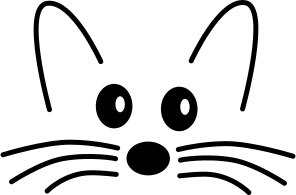
\includegraphics[width=1.4em]{squeak-logo}}}
\iftoshelse{
	\usepackage{marginnote}
		\renewcommand*{\marginfont}{\footnotesize}
	\newcommand{\vartriangleout}{\ifthenelse{\isodd{\thepage}}{\vartriangleright}{\vartriangleleft}}
	\newcommand{\dothisicon}{\fcolorbox{blue!65}{white}{\highlight{$\vartriangleout$}}}
	\newcommand{\dothis}[1]{%
		\noindent\par\noindent
		{\reversemarginpar
			\marginnote{\fcolorbox{blue!65}{white}{\highlight{$\vartriangleout$}}}}
		%\MarginLabel{do this}
		\noindent\emph{#1}
		\nopagebreak}
}{
	\newcommand{\dothisicon}{\raisebox{-.5ex}{
\includegraphics[height=1.2em]{pharo}}}
	\newcommand{\dothis}[1]{%
		\medskip
		\noindent\dothisicon
		\ifx#1\empty\else\quad\emph{#1}\fi
		\par\smallskip\nopagebreak}
}
%===> NEW VERSION <===
% NB: To use this in an individual chapter, you must set:
%\graphicspath{{figures/} {../figures/}}
% at the head of the chapter.  Don't forget the final /
%=============================================================
%:Reader hints (hint)
%
% Indicates a non-obvious consequence 
\newcommand{\hint}[1]{\vspace{1ex}\noindent\fbox{\textsc{Hint}} \emph{#1}}
%=================================================================
% graphics for Morphic handles
\newcommand{\grabHandle}{\raisebox{-0.2ex}{
\includegraphics[width=1em]{blackHandle}}}
\newcommand{\moveHandle}{\raisebox{-0.2ex}{
\includegraphics[width=1em]{moveHandle}}}
\newcommand{\debugHandle}{\raisebox{-0.2ex}{
\includegraphics[width=1em]{debugHandle}}}
%=============================================================
%:Highlighting Important stuff (doublebox)
%
% From Seaside book ...
\newsavebox{\SavedText}
\newlength{\InnerBoxRule}\setlength{\InnerBoxRule}{.75\fboxrule}
\newlength{\OuterBoxRule}\setlength{\OuterBoxRule}{1.5\fboxrule}
\newlength{\BoxSeparation}\setlength{\BoxSeparation}{1.5\fboxrule}
\addtolength{\BoxSeparation}{.5pt}
\newlength{\SaveBoxSep}\setlength{\SaveBoxSep}{2\fboxsep}
%
\newenvironment{doublebox}{\begin{lrbox}{\SavedText}
    \begin{minipage}{.75\textwidth}}
    {\end{minipage}\end{lrbox}\begin{center}
    \setlength{\fboxsep}{\BoxSeparation}\setlength{\fboxrule}{\OuterBoxRule}
    \fbox{\setlength{\fboxsep}{\SaveBoxSep}\setlength{\fboxrule}{\InnerBoxRule}%
      \fbox{\usebox{\SavedText}}}
  \end{center}}
% Use this:
\newcommand{\important}[1]{\begin{doublebox}#1\end{doublebox}}
%=============================================================
%:Section depth
\setcounter{secnumdepth}{2}
%% for this to happen start the file with
%\ifx\wholebook\relax\else
%% $Author$
% $Date$
% $Revision$

% HISTORY:
% 2006-10-31 - Oscar code macros
% ...

%=============================================================
% NB: documentclass must be set in main document.
% Allows book to be generated in multiple formats.
%=============================================================
%:Packages
\usepackage[T1]{fontenc}  %%%%%% really important to get the code directly in the text!
\usepackage{lmodern}
%\usepackage[scaled=0.85]{bookmanx} % needs another scale factor if used with \renewcommand{\sfdefault}{cmbr}
\usepackage{palatino}
\usepackage[scaled=0.85]{helvet}
\usepackage[protrusion,expansion=false]{microtype}
\usepackage{graphicx}
\usepackage{theorem}
\usepackage[english]{babel}
%%% ON: pdfsync breaks the use of p{width} for tabular columns!
%%\ifdefined\usepdfsync\usepackage{pdfsync}\fi % Requires texlive 2007
%=============================================================
%:More packages
%Stef should check which ones are used!
%\usepackage{picinpar}
%\usepackage{layout}
%\usepackage{color}
%\usepackage{enum}
%\usepackage{a4wide}
% \usepackage{fancyhdr}
\usepackage{ifthen}
\usepackage{float}
\usepackage{longtable}
\usepackage{makeidx}
\usepackage[nottoc]{tocbibind}
\usepackage{multicol}
\usepackage{booktabs}	% book-style tables
\usepackage{topcapt}	% enables \topcaption
\usepackage{multirow}
\usepackage{tabularx}
%\usepackage[bottom]{footmisc}
\usepackage{xspace}
\usepackage{alltt}
\usepackage{amssymb,textcomp}
\usepackage[usenames,dvipsnames]{color}
%\usepackage{colortbl}
\usepackage[hang]{subfigure}\makeatletter\def\p@subfigure{\thefigure\,}\makeatother
\usepackage{rotating}
\usepackage{enumitem}	% apb: allows more control over tags in enumerations
\usepackage{verbatim}     % for comment environment
\usepackage{varioref}	% for page references that work
\labelformat{footnote}{\thechapter--#1} % to distinguish citations from jurabib
\usepackage{needspace}
\usepackage{isodateo} % enable \isodate
\usepackage[newparttoc]{titlesec}
\usepackage{titletoc}
\usepackage{wrapfig}
\usepackage[
	super,
	citefull=first,
	authorformat={allreversed,and},
	titleformat={commasep,italic}
]{jurabib} % citations as footnotes
\usepackage[
	colorlinks=true,
	linkcolor=black,
	urlcolor=black,
	citecolor=black
]{hyperref}   % should come last
%=============================================================
%:PDF version
%%\pdfminorversion=3 % Set PDF to 1.3 for Lulu
%=============================================================
%:URL style
\makeatletter
\def\url@leostyle{%
  \@ifundefined{selectfont}{\def\UrlFont{\sf}}{\def\UrlFont{\sffamily}}}
\makeatother
% Now actually use the newly defined style.
\urlstyle{leo}
%=============================================================
%:Booleans
\newboolean{lulu}
\setboolean{lulu}{false}
\newcommand{\ifluluelse}[2]{\ifthenelse{\boolean{lulu}}{#1}{#2}}
%=============================================================
%:Names
\newcommand{\SUnit}{SUnit\xspace}
\newcommand{\sunit}{SUnit\xspace}
\newcommand{\xUnit}{$x$Unit\xspace}
\newcommand{\JUnit}{JUnit\xspace}
\newcommand{\st}{Smalltalk\xspace}
\newcommand{\pharo}{Pharo\xspace} % Use this, not \Pharo
%\newcommand{\sqmap}{SqueakMap\xspace}
\newcommand{\squeak}{Squeak\xspace} % use this, not \Squeak or \sq
\newcommand{\sqsrc}{SqueakSource\xspace}
\newcommand{\sbe}{\url{http://SqueakByExample.org}\xspace}
\newcommand{\pharoweb}{\url{http://pharo-project.org}\xspace}
\newcommand{\pbe}{\url{http://PharoByExample.org}\xspace}
\newcommand{\sba}{\url{http://SquareBracketAssociates.org}\xspace}
\newcommand{\bam}{\lct{Bounc\-ing\-Atoms\-Morph}\xspace}
%=============================================================
%:Markup macros for proof-reading
\usepackage[normalem]{ulem} % for \sout
\usepackage{xcolor}
\newcommand{\ra}{$\rightarrow$}
\newcommand{\ugh}[1]{\textcolor{red}{\uwave{#1}}} % please rephrase
\newcommand{\ins}[1]{\textcolor{blue}{\uline{#1}}} % please insert
\newcommand{\del}[1]{\textcolor{red}{\sout{#1}}} % please delete
\newcommand{\chg}[2]{\textcolor{red}{\sout{#1}}{\ra}\textcolor{blue}{\uline{#2}}} % please change
%=============================================================
%:Editorial comment macros
%\newcommand{\nnbb}[2]{
%    % \fbox{\bfseries\sffamily\scriptsize#1}
%    \fcolorbox{gray}{yellow}{\bfseries\sffamily\scriptsize#1}
%    {\sf\small$\blacktriangleright$\textit{#2}$\blacktriangleleft$}
%   }
\newcommand{\yellowbox}[1]{\fcolorbox{gray}{yellow}{\bfseries\sffamily\scriptsize#1}}
\newcommand{\triangles}[1]{{\sf\small$\blacktriangleright$\textit{#1}$\blacktriangleleft$}}
\newcommand{\nnbb}[2]{\yellowbox{#1} \triangles{#2}}
\newcommand{\fix}{\yellowbox{FIX!}}
\newcommand{\here}{\yellowbox{CONTINUE HERE!}}
% editor macros
\newcommand{\apl}[1]{\nnbb{Alain}{#1}} % Alain
\newcommand{\ab}[1]{\nnbb{Andrew}{#1}} % Black
\newcommand{\sd}[1]{\nnbb{St\'{e}f}{#1}} % Ducasse
\newcommand{\dc}[1]{\nnbb{DamienC}{#1}} % Ducasse
\newcommand{\md}[1]{\nnbb{Marcus}{#1}} % Denker
\newcommand{\on}[1]{\nnbb{Oscar}{#1}} % Nierstrasz
\newcommand{\damien}[1]{\nnbb{Damien}{#1}} % Pollet
\newcommand{\lr}[1]{\nnbb{Lukas}{#1}} % Renggli
\newcommand{\orla}[1]{\nnbb{Orla}{#1}} % Greevy
\newcommand{\alex}[1]{\nnbb{Alex}{#1}} % Bergel
\newcommand{\alx}[1]{\nnbb{Alex}{#1}} % Bergel
\newcommand{\dr}[1]{\nnbb{David}{#1}} % Roethlisberger
\newcommand{\ja}[1]{\nnbb{Jannik}{#1}} % Laval
\newcommand{\jr}[1]{\nnbb{Jorge}{#1}} % Ressia
\newcommand{\fp}[1]{\nnbb{Fabrizio}{#1}} % Perin
\newcommand{\michael}[1]{\nnbb{Michael}{#1}} % Davies
\newcommand{\ew}[1]{\nnbb{Erwann}{#1}} % Wernli
\newcommand{\mb}[1]{\nnbb{Martial}{#1}} % Boniou
\newcommand{\hw}[1]{\nnbb{Hernan}{#1}} % Wilkinson
%=============================================================
%:Abbreviation macros
\newcommand{\ie}{\emph{すなわち}、}
\newcommand{\eg}{\emph{例えば}、}
\newcommand{\etc}{などなど。}
%=============================================================
%:Cross reference macros
\newcommand{\charef}[1]{第~\ref{cha:#1}~章}
\newcommand{\secref}[1]{\ref{sec:#1}~節}
\newcommand{\figref}[1]{図~\ref{fig:#1}\xspace}
\newcommand{\Figref}[1]{図~\ref{fig:#1}\xspace}
\newcommand{\appref}[1]{付録~\ref{app:#1}\xspace}
\newcommand{\tabref}[1]{表~\ref{tab:#1}\xspace}
\newcommand{\faqref}[1]{FAQ~\ref{faq:#1}, p.~\pageref{faq:#1}\xspace}
% APB: I removed trailing \xspace commands from these macros because
% \xspace mostly doesn't work.  If you want a space after your
% references, type one!
% ON: xspace has always worked just fine for me!  Please leave them in.
%
\newcommand{\ruleref}[1]{\ref{rule:#1}\xspace}
%
\newcommand{\egref}[1]{example~\ref{eg:#1}\xspace}
\newcommand{\Egref}[1]{Example~\ref{eg:#1}\xspace}
%
\newcommand{\scrref}[1]{script~\ref{scr:#1}\xspace}
\newcommand{\Scrref}[1]{Script~\ref{scr:#1}\xspace}
\newcommand{\tscrref}[1]{the script~\ref{scr:#1}\xspace}
\newcommand{\Tscrref}[1]{The script~\ref{scr:#1}\xspace}
%
\newcommand{\mthref}[1]{method~\ref{mth:#1}\xspace}
\newcommand{\mthsref}[1]{methods~\ref{mth:#1}\xspace}
\newcommand{\Mthref}[1]{Method~\ref{mth:#1}\xspace}
\newcommand{\tmthref}[1]{the method~\ref{mth:#1}\xspace}
\newcommand{\Tmthref}[1]{The method~\ref{mth:#1}\xspace}
%
\newcommand{\clsref}[1]{class~\ref{cls:#1}\xspace}
\newcommand{\tclsref}[1]{the class~\ref{cls:#1}\xspace}
\newcommand{\Tclsref}[1]{The class~\ref{cls:#1}\xspace}

\newcommand{\chalabel}[1]{\label{cha:#1}}
\newcommand{\seclabel}[1]{\label{sec:#1}}
\newcommand{\figlabel}[1]{\label{fig:#1}}
\newcommand{\tablabel}[1]{\label{tab:#1}}
\newcommand{\rulelabel}[1]{\label{rule:#1}}
\newcommand{\eglabel}[1]{\label{eg:#1}}
\newcommand{\scrlabel}[1]{\label{scr:#1}}
\newcommand{\mthlabel}[1]{\label{mth:#1}}
\newcommand{\clslabel}[1]{\label{cls:#1}}
\newcommand{\faqlabel}[1]{\label{faq:#1}}
%=============================================================
%:Menu item macro
% for menu items, so we can change our minds on how to print them! (apb)
\definecolor{lightgray}{gray}{0.89}
\newcommand{\menu}[1]{{%
	\setlength{\fboxsep}{0pt}%
	\colorbox{lightgray}{{{\upshape\sffamily\strut \,#1\,}}}}}
\newcommand{\link}[1]{{%
	\fontfamily{lmr}\selectfont
 	\upshape{\sffamily \underline{#1}}}}
% For submenu items:
\newcommand{\go}{\,$\triangleright$\,}
% \newcommand{\go}{\,$\blacktriangleright$\,}
% For keyboard shortcuts:
%\newcommand{\short}[1]{\mbox{$\langle${\sc CMD}$\rangle$-#1}\xspace}
\newcommand{\short}[1]{\mbox{{\sc cmd}\hspace{0.08em}--\hspace{0.09em}#1}\xspace}
% For buttons:
\newcommand{\button}[1]{{%
	\setlength{\fboxsep}{0pt}%
	\fbox{{\upshape\sffamily\strut \,#1\,}}}}
% NB: The button macro does not work within captions -- incompatible with xcolor package :-(
\newcommand{\toolsflap}{\textit{Tools} flap\xspace}
%=============================================================
%:Mouse clicks
\newcommand{\click}{click\xspace} % RED
\newcommand{\actclick}{action-click\xspace} % YELLOW
\newcommand{\metaclick}{meta-click\xspace} % BLUE
\newcommand{\Click}{Click\xspace} % RED
\newcommand{\Actclick}{Action-click\xspace} % YELLOW
\newcommand{\Metaclick}{Meta-click\xspace} % BLUE
%=============================================================
%:ToSh macros
\newboolean{tosh}
\setboolean{tosh}{false}
\newcommand{\iftoshelse}[2]{\ifthenelse{\boolean{tosh}}{#1}{#2}}
%=============================================================
%:ToSh colors
%\newcommand{\highlightcolor}{\color{blue!65}}
%\newcommand{\boxcolor}{\color{gray!25}}
\newcommand{\highlight}[1]{\textcolor{blue!65}{#1}}
%\newcommand{\codecolor}{\color{blue!65}}
%%\setlength{\fboxrule}{2pt}
%\newcommand{\asPict}[1]{%
%	{\Large\highlight{#1}}}
%=============================================================
%:Reader cues (do this)
%
% Indicate something the reader should try out.
% \newcommand{\dothisicon}{\raisebox{-.5ex}{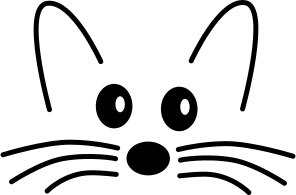
\includegraphics[width=1.4em]{squeak-logo}}}
\iftoshelse{
	\usepackage{marginnote}
		\renewcommand*{\marginfont}{\footnotesize}
	\newcommand{\vartriangleout}{\ifthenelse{\isodd{\thepage}}{\vartriangleright}{\vartriangleleft}}
	\newcommand{\dothisicon}{\fcolorbox{blue!65}{white}{\highlight{$\vartriangleout$}}}
	\newcommand{\dothis}[1]{%
		\noindent\par\noindent
		{\reversemarginpar
			\marginnote{\fcolorbox{blue!65}{white}{\highlight{$\vartriangleout$}}}}
		%\MarginLabel{do this}
		\noindent\emph{#1}
		\nopagebreak}
}{
	\newcommand{\dothisicon}{\raisebox{-.5ex}{
\includegraphics[height=1.2em]{pharo}}}
	\newcommand{\dothis}[1]{%
		\medskip
		\noindent\dothisicon
		\ifx#1\empty\else\quad\emph{#1}\fi
		\par\smallskip\nopagebreak}
}
%===> NEW VERSION <===
% NB: To use this in an individual chapter, you must set:
%\graphicspath{{figures/} {../figures/}}
% at the head of the chapter.  Don't forget the final /
%=============================================================
%:Reader hints (hint)
%
% Indicates a non-obvious consequence 
\newcommand{\hint}[1]{\vspace{1ex}\noindent\fbox{\textsc{Hint}} \emph{#1}}
%=================================================================
% graphics for Morphic handles
\newcommand{\grabHandle}{\raisebox{-0.2ex}{
\includegraphics[width=1em]{blackHandle}}}
\newcommand{\moveHandle}{\raisebox{-0.2ex}{
\includegraphics[width=1em]{moveHandle}}}
\newcommand{\debugHandle}{\raisebox{-0.2ex}{
\includegraphics[width=1em]{debugHandle}}}
%=============================================================
%:Highlighting Important stuff (doublebox)
%
% From Seaside book ...
\newsavebox{\SavedText}
\newlength{\InnerBoxRule}\setlength{\InnerBoxRule}{.75\fboxrule}
\newlength{\OuterBoxRule}\setlength{\OuterBoxRule}{1.5\fboxrule}
\newlength{\BoxSeparation}\setlength{\BoxSeparation}{1.5\fboxrule}
\addtolength{\BoxSeparation}{.5pt}
\newlength{\SaveBoxSep}\setlength{\SaveBoxSep}{2\fboxsep}
%
\newenvironment{doublebox}{\begin{lrbox}{\SavedText}
    \begin{minipage}{.75\textwidth}}
    {\end{minipage}\end{lrbox}\begin{center}
    \setlength{\fboxsep}{\BoxSeparation}\setlength{\fboxrule}{\OuterBoxRule}
    \fbox{\setlength{\fboxsep}{\SaveBoxSep}\setlength{\fboxrule}{\InnerBoxRule}%
      \fbox{\usebox{\SavedText}}}
  \end{center}}
% Use this:
\newcommand{\important}[1]{\begin{doublebox}#1\end{doublebox}}
%=============================================================
%:Section depth
\setcounter{secnumdepth}{2}
%% for this to happen start the file with
%\ifx\wholebook\relax\else
%% $Author$
% $Date$
% $Revision$

% HISTORY:
% 2006-10-31 - Oscar code macros
% ...

%=============================================================
% NB: documentclass must be set in main document.
% Allows book to be generated in multiple formats.
%=============================================================
%:Packages
\usepackage[T1]{fontenc}  %%%%%% really important to get the code directly in the text!
\usepackage{lmodern}
%\usepackage[scaled=0.85]{bookmanx} % needs another scale factor if used with \renewcommand{\sfdefault}{cmbr}
\usepackage{palatino}
\usepackage[scaled=0.85]{helvet}
\usepackage[protrusion,expansion=false]{microtype}
\usepackage{graphicx}
\usepackage{theorem}
\usepackage[english]{babel}
%%% ON: pdfsync breaks the use of p{width} for tabular columns!
%%\ifdefined\usepdfsync\usepackage{pdfsync}\fi % Requires texlive 2007
%=============================================================
%:More packages
%Stef should check which ones are used!
%\usepackage{picinpar}
%\usepackage{layout}
%\usepackage{color}
%\usepackage{enum}
%\usepackage{a4wide}
% \usepackage{fancyhdr}
\usepackage{ifthen}
\usepackage{float}
\usepackage{longtable}
\usepackage{makeidx}
\usepackage[nottoc]{tocbibind}
\usepackage{multicol}
\usepackage{booktabs}	% book-style tables
\usepackage{topcapt}	% enables \topcaption
\usepackage{multirow}
\usepackage{tabularx}
%\usepackage[bottom]{footmisc}
\usepackage{xspace}
\usepackage{alltt}
\usepackage{amssymb,textcomp}
\usepackage[usenames,dvipsnames]{color}
%\usepackage{colortbl}
\usepackage[hang]{subfigure}\makeatletter\def\p@subfigure{\thefigure\,}\makeatother
\usepackage{rotating}
\usepackage{enumitem}	% apb: allows more control over tags in enumerations
\usepackage{verbatim}     % for comment environment
\usepackage{varioref}	% for page references that work
\labelformat{footnote}{\thechapter--#1} % to distinguish citations from jurabib
\usepackage{needspace}
\usepackage{isodateo} % enable \isodate
\usepackage[newparttoc]{titlesec}
\usepackage{titletoc}
\usepackage{wrapfig}
\usepackage[
	super,
	citefull=first,
	authorformat={allreversed,and},
	titleformat={commasep,italic}
]{jurabib} % citations as footnotes
\usepackage[
	colorlinks=true,
	linkcolor=black,
	urlcolor=black,
	citecolor=black
]{hyperref}   % should come last
%=============================================================
%:PDF version
%%\pdfminorversion=3 % Set PDF to 1.3 for Lulu
%=============================================================
%:URL style
\makeatletter
\def\url@leostyle{%
  \@ifundefined{selectfont}{\def\UrlFont{\sf}}{\def\UrlFont{\sffamily}}}
\makeatother
% Now actually use the newly defined style.
\urlstyle{leo}
%=============================================================
%:Booleans
\newboolean{lulu}
\setboolean{lulu}{false}
\newcommand{\ifluluelse}[2]{\ifthenelse{\boolean{lulu}}{#1}{#2}}
%=============================================================
%:Names
\newcommand{\SUnit}{SUnit\xspace}
\newcommand{\sunit}{SUnit\xspace}
\newcommand{\xUnit}{$x$Unit\xspace}
\newcommand{\JUnit}{JUnit\xspace}
\newcommand{\st}{Smalltalk\xspace}
\newcommand{\pharo}{Pharo\xspace} % Use this, not \Pharo
%\newcommand{\sqmap}{SqueakMap\xspace}
\newcommand{\squeak}{Squeak\xspace} % use this, not \Squeak or \sq
\newcommand{\sqsrc}{SqueakSource\xspace}
\newcommand{\sbe}{\url{http://SqueakByExample.org}\xspace}
\newcommand{\pharoweb}{\url{http://pharo-project.org}\xspace}
\newcommand{\pbe}{\url{http://PharoByExample.org}\xspace}
\newcommand{\sba}{\url{http://SquareBracketAssociates.org}\xspace}
\newcommand{\bam}{\lct{Bounc\-ing\-Atoms\-Morph}\xspace}
%=============================================================
%:Markup macros for proof-reading
\usepackage[normalem]{ulem} % for \sout
\usepackage{xcolor}
\newcommand{\ra}{$\rightarrow$}
\newcommand{\ugh}[1]{\textcolor{red}{\uwave{#1}}} % please rephrase
\newcommand{\ins}[1]{\textcolor{blue}{\uline{#1}}} % please insert
\newcommand{\del}[1]{\textcolor{red}{\sout{#1}}} % please delete
\newcommand{\chg}[2]{\textcolor{red}{\sout{#1}}{\ra}\textcolor{blue}{\uline{#2}}} % please change
%=============================================================
%:Editorial comment macros
%\newcommand{\nnbb}[2]{
%    % \fbox{\bfseries\sffamily\scriptsize#1}
%    \fcolorbox{gray}{yellow}{\bfseries\sffamily\scriptsize#1}
%    {\sf\small$\blacktriangleright$\textit{#2}$\blacktriangleleft$}
%   }
\newcommand{\yellowbox}[1]{\fcolorbox{gray}{yellow}{\bfseries\sffamily\scriptsize#1}}
\newcommand{\triangles}[1]{{\sf\small$\blacktriangleright$\textit{#1}$\blacktriangleleft$}}
\newcommand{\nnbb}[2]{\yellowbox{#1} \triangles{#2}}
\newcommand{\fix}{\yellowbox{FIX!}}
\newcommand{\here}{\yellowbox{CONTINUE HERE!}}
% editor macros
\newcommand{\apl}[1]{\nnbb{Alain}{#1}} % Alain
\newcommand{\ab}[1]{\nnbb{Andrew}{#1}} % Black
\newcommand{\sd}[1]{\nnbb{St\'{e}f}{#1}} % Ducasse
\newcommand{\dc}[1]{\nnbb{DamienC}{#1}} % Ducasse
\newcommand{\md}[1]{\nnbb{Marcus}{#1}} % Denker
\newcommand{\on}[1]{\nnbb{Oscar}{#1}} % Nierstrasz
\newcommand{\damien}[1]{\nnbb{Damien}{#1}} % Pollet
\newcommand{\lr}[1]{\nnbb{Lukas}{#1}} % Renggli
\newcommand{\orla}[1]{\nnbb{Orla}{#1}} % Greevy
\newcommand{\alex}[1]{\nnbb{Alex}{#1}} % Bergel
\newcommand{\alx}[1]{\nnbb{Alex}{#1}} % Bergel
\newcommand{\dr}[1]{\nnbb{David}{#1}} % Roethlisberger
\newcommand{\ja}[1]{\nnbb{Jannik}{#1}} % Laval
\newcommand{\jr}[1]{\nnbb{Jorge}{#1}} % Ressia
\newcommand{\fp}[1]{\nnbb{Fabrizio}{#1}} % Perin
\newcommand{\michael}[1]{\nnbb{Michael}{#1}} % Davies
\newcommand{\ew}[1]{\nnbb{Erwann}{#1}} % Wernli
\newcommand{\mb}[1]{\nnbb{Martial}{#1}} % Boniou
\newcommand{\hw}[1]{\nnbb{Hernan}{#1}} % Wilkinson
%=============================================================
%:Abbreviation macros
\newcommand{\ie}{\emph{すなわち}、}
\newcommand{\eg}{\emph{例えば}、}
\newcommand{\etc}{などなど。}
%=============================================================
%:Cross reference macros
\newcommand{\charef}[1]{第~\ref{cha:#1}~章}
\newcommand{\secref}[1]{\ref{sec:#1}~節}
\newcommand{\figref}[1]{図~\ref{fig:#1}\xspace}
\newcommand{\Figref}[1]{図~\ref{fig:#1}\xspace}
\newcommand{\appref}[1]{付録~\ref{app:#1}\xspace}
\newcommand{\tabref}[1]{表~\ref{tab:#1}\xspace}
\newcommand{\faqref}[1]{FAQ~\ref{faq:#1}, p.~\pageref{faq:#1}\xspace}
% APB: I removed trailing \xspace commands from these macros because
% \xspace mostly doesn't work.  If you want a space after your
% references, type one!
% ON: xspace has always worked just fine for me!  Please leave them in.
%
\newcommand{\ruleref}[1]{\ref{rule:#1}\xspace}
%
\newcommand{\egref}[1]{example~\ref{eg:#1}\xspace}
\newcommand{\Egref}[1]{Example~\ref{eg:#1}\xspace}
%
\newcommand{\scrref}[1]{script~\ref{scr:#1}\xspace}
\newcommand{\Scrref}[1]{Script~\ref{scr:#1}\xspace}
\newcommand{\tscrref}[1]{the script~\ref{scr:#1}\xspace}
\newcommand{\Tscrref}[1]{The script~\ref{scr:#1}\xspace}
%
\newcommand{\mthref}[1]{method~\ref{mth:#1}\xspace}
\newcommand{\mthsref}[1]{methods~\ref{mth:#1}\xspace}
\newcommand{\Mthref}[1]{Method~\ref{mth:#1}\xspace}
\newcommand{\tmthref}[1]{the method~\ref{mth:#1}\xspace}
\newcommand{\Tmthref}[1]{The method~\ref{mth:#1}\xspace}
%
\newcommand{\clsref}[1]{class~\ref{cls:#1}\xspace}
\newcommand{\tclsref}[1]{the class~\ref{cls:#1}\xspace}
\newcommand{\Tclsref}[1]{The class~\ref{cls:#1}\xspace}

\newcommand{\chalabel}[1]{\label{cha:#1}}
\newcommand{\seclabel}[1]{\label{sec:#1}}
\newcommand{\figlabel}[1]{\label{fig:#1}}
\newcommand{\tablabel}[1]{\label{tab:#1}}
\newcommand{\rulelabel}[1]{\label{rule:#1}}
\newcommand{\eglabel}[1]{\label{eg:#1}}
\newcommand{\scrlabel}[1]{\label{scr:#1}}
\newcommand{\mthlabel}[1]{\label{mth:#1}}
\newcommand{\clslabel}[1]{\label{cls:#1}}
\newcommand{\faqlabel}[1]{\label{faq:#1}}
%=============================================================
%:Menu item macro
% for menu items, so we can change our minds on how to print them! (apb)
\definecolor{lightgray}{gray}{0.89}
\newcommand{\menu}[1]{{%
	\setlength{\fboxsep}{0pt}%
	\colorbox{lightgray}{{{\upshape\sffamily\strut \,#1\,}}}}}
\newcommand{\link}[1]{{%
	\fontfamily{lmr}\selectfont
 	\upshape{\sffamily \underline{#1}}}}
% For submenu items:
\newcommand{\go}{\,$\triangleright$\,}
% \newcommand{\go}{\,$\blacktriangleright$\,}
% For keyboard shortcuts:
%\newcommand{\short}[1]{\mbox{$\langle${\sc CMD}$\rangle$-#1}\xspace}
\newcommand{\short}[1]{\mbox{{\sc cmd}\hspace{0.08em}--\hspace{0.09em}#1}\xspace}
% For buttons:
\newcommand{\button}[1]{{%
	\setlength{\fboxsep}{0pt}%
	\fbox{{\upshape\sffamily\strut \,#1\,}}}}
% NB: The button macro does not work within captions -- incompatible with xcolor package :-(
\newcommand{\toolsflap}{\textit{Tools} flap\xspace}
%=============================================================
%:Mouse clicks
\newcommand{\click}{click\xspace} % RED
\newcommand{\actclick}{action-click\xspace} % YELLOW
\newcommand{\metaclick}{meta-click\xspace} % BLUE
\newcommand{\Click}{Click\xspace} % RED
\newcommand{\Actclick}{Action-click\xspace} % YELLOW
\newcommand{\Metaclick}{Meta-click\xspace} % BLUE
%=============================================================
%:ToSh macros
\newboolean{tosh}
\setboolean{tosh}{false}
\newcommand{\iftoshelse}[2]{\ifthenelse{\boolean{tosh}}{#1}{#2}}
%=============================================================
%:ToSh colors
%\newcommand{\highlightcolor}{\color{blue!65}}
%\newcommand{\boxcolor}{\color{gray!25}}
\newcommand{\highlight}[1]{\textcolor{blue!65}{#1}}
%\newcommand{\codecolor}{\color{blue!65}}
%%\setlength{\fboxrule}{2pt}
%\newcommand{\asPict}[1]{%
%	{\Large\highlight{#1}}}
%=============================================================
%:Reader cues (do this)
%
% Indicate something the reader should try out.
% \newcommand{\dothisicon}{\raisebox{-.5ex}{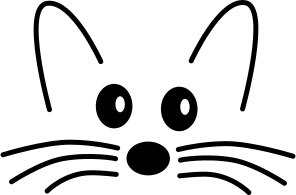
\includegraphics[width=1.4em]{squeak-logo}}}
\iftoshelse{
	\usepackage{marginnote}
		\renewcommand*{\marginfont}{\footnotesize}
	\newcommand{\vartriangleout}{\ifthenelse{\isodd{\thepage}}{\vartriangleright}{\vartriangleleft}}
	\newcommand{\dothisicon}{\fcolorbox{blue!65}{white}{\highlight{$\vartriangleout$}}}
	\newcommand{\dothis}[1]{%
		\noindent\par\noindent
		{\reversemarginpar
			\marginnote{\fcolorbox{blue!65}{white}{\highlight{$\vartriangleout$}}}}
		%\MarginLabel{do this}
		\noindent\emph{#1}
		\nopagebreak}
}{
	\newcommand{\dothisicon}{\raisebox{-.5ex}{
\includegraphics[height=1.2em]{pharo}}}
	\newcommand{\dothis}[1]{%
		\medskip
		\noindent\dothisicon
		\ifx#1\empty\else\quad\emph{#1}\fi
		\par\smallskip\nopagebreak}
}
%===> NEW VERSION <===
% NB: To use this in an individual chapter, you must set:
%\graphicspath{{figures/} {../figures/}}
% at the head of the chapter.  Don't forget the final /
%=============================================================
%:Reader hints (hint)
%
% Indicates a non-obvious consequence 
\newcommand{\hint}[1]{\vspace{1ex}\noindent\fbox{\textsc{Hint}} \emph{#1}}
%=================================================================
% graphics for Morphic handles
\newcommand{\grabHandle}{\raisebox{-0.2ex}{
\includegraphics[width=1em]{blackHandle}}}
\newcommand{\moveHandle}{\raisebox{-0.2ex}{
\includegraphics[width=1em]{moveHandle}}}
\newcommand{\debugHandle}{\raisebox{-0.2ex}{
\includegraphics[width=1em]{debugHandle}}}
%=============================================================
%:Highlighting Important stuff (doublebox)
%
% From Seaside book ...
\newsavebox{\SavedText}
\newlength{\InnerBoxRule}\setlength{\InnerBoxRule}{.75\fboxrule}
\newlength{\OuterBoxRule}\setlength{\OuterBoxRule}{1.5\fboxrule}
\newlength{\BoxSeparation}\setlength{\BoxSeparation}{1.5\fboxrule}
\addtolength{\BoxSeparation}{.5pt}
\newlength{\SaveBoxSep}\setlength{\SaveBoxSep}{2\fboxsep}
%
\newenvironment{doublebox}{\begin{lrbox}{\SavedText}
    \begin{minipage}{.75\textwidth}}
    {\end{minipage}\end{lrbox}\begin{center}
    \setlength{\fboxsep}{\BoxSeparation}\setlength{\fboxrule}{\OuterBoxRule}
    \fbox{\setlength{\fboxsep}{\SaveBoxSep}\setlength{\fboxrule}{\InnerBoxRule}%
      \fbox{\usebox{\SavedText}}}
  \end{center}}
% Use this:
\newcommand{\important}[1]{\begin{doublebox}#1\end{doublebox}}
%=============================================================
%:Section depth
\setcounter{secnumdepth}{2}
%% for this to happen start the file with
%\ifx\wholebook\relax\else
%\input{../common.tex}
%\begin{document}
%\fi
% and terminate by
% \ifx\wholebook\relax\else\end{document}\fi

\DeclareGraphicsExtensions{.pdf, .jpg, .png}
%=============================================================
%:PDF setup
\hypersetup{
%   a4paper,
%   pdfstartview=FitV,
%   colorlinks,
%   linkcolor=darkblue,
%   citecolor=darkblue,
   pdftitle={Pharo by Example},
   pdfauthor={Andrew P. Black, St\'ephane Ducasse,	Oscar Nierstrasz,
Damien Pollet},
   pdfkeywords={Smalltalk, Squeak, Object-Oriented Programming, OOP},
   pdfsubject={Computer Science}
}
%=============================================================
%:Page layout and appearance
%
% \renewcommand{\headrulewidth}{0pt}
\renewcommand{\chaptermark}[1]{\markboth{#1}{}}
\renewcommand{\sectionmark}[1]{\markright{\thesection\ #1}}
\renewpagestyle{plain}[\small\itshape]{%
	\setheadrule{0pt}%
	\sethead[][][]{}{}{}%
	\setfoot[][][]{}{}{}}
\renewpagestyle{headings}[\small\itshape]{%
	\setheadrule{0pt}%
	\setmarks{chapter}{section}%
	\sethead[\thepage][][\chaptertitle]{\sectiontitle}{}{\thepage}%
	\setfoot[][][]{}{}{}}
%=============================================================
%:Title section setup and TOC numbering depth
\setcounter{secnumdepth}{1}
\setcounter{tocdepth}{1}
\titleformat{\part}[display]{\centering}{\huge\partname\ \thepart}{1em}{\Huge\textbf}[]
\titleformat{\chapter}[display]{}{\huge\chaptertitlename\ \thechapter}{1em}{\Huge\raggedright\textbf}[]
\titlecontents{part}[3pc]{%
		\pagebreak[2]\addvspace{1em plus.4em minus.2em}%
		\leavevmode\large\bfseries}
	{\contentslabel{3pc}}{\hspace*{-3pc}}
	{}[\nopagebreak]
\titlecontents{chapter}[3pc]{%
		\pagebreak[0]\addvspace{1em plus.2em minus.2em}%
		\leavevmode\bfseries}
	{\contentslabel{3pc}}{}
	{\hfill\contentspage}[\nopagebreak]
\dottedcontents{section}[3pc]{}{3pc}{1pc}
\dottedcontents{subsection}[3pc]{}{0pc}{1pc}
% \dottedcontents{subsection}[4.5em]{}{0pt}{1pc}
% Make \cleardoublepage insert really blank pages http://www.tex.ac.uk/cgi-bin/texfaq2html?label=reallyblank
\let\origdoublepage\cleardoublepage
\newcommand{\clearemptydoublepage}{%
  \clearpage
  {\pagestyle{empty}\origdoublepage}}
\let\cleardoublepage\clearemptydoublepage % see http://www.tex.ac.uk/cgi-bin/texfaq2html?label=patch
%=============================================================
%:FAQ macros (for FAQ chapter)
\newtheorem{faq}{FAQ}
\newcommand{\answer}{\paragraph{Answer}\ }
%=============================================================
%:Listings package configuration
% \newcommand{\caret}{\makebox{\raisebox{0.4ex}{\footnotesize{$\wedge$}}}}
\newcommand{\caret}{\^\,}
\newcommand{\escape}{{\sf \textbackslash}}
\definecolor{source}{gray}{0.95}
\usepackage{listings}
\lstdefinelanguage{Smalltalk}{
%  morekeywords={self,super,true,false,nil,thisContext}, % This is overkill
  morestring=[d]',
  morecomment=[s]{"}{"},
  alsoletter={\#:},
  escapechar={!},
  literate=
    {BANG}{!}1
    {CARET}{\^}1
    {UNDERSCORE}{\_}1
    {\\st}{Smalltalk}9 % convenience -- in case \st occurs in code
    % {'}{{\textquotesingle}}1 % replaced by upquote=true in \lstset
    {_}{{$\leftarrow$}}1
    {>>>}{{\sep}}1
    {^}{{$\uparrow$}}1
    {~}{{$\sim$}}1
    {-}{{\texttt{-}}}1 %{\textminus}}1 %{-}{\hspace{-0.13em}}{-}}1  % the goal is to make - the same width as +
    % {+}{\sf+}1 %{\raisebox{0.08ex}{+}}}1      % and to raise + off the baseline to match -
    {-->}{{\quad$\longrightarrow$\quad}}3
	, % Don't forget the comma at the end!
  tabsize=4
}[keywords,comments,strings]

\lstset{language=Smalltalk,
	basicstyle=\sffamily,
	keywordstyle=\color{black}\bfseries,
	% stringstyle=\ttfamily, % Ugly! do we really want this? -- on
	mathescape=true,
	showstringspaces=false,
	keepspaces=true,
	breaklines=true,
	breakautoindent=true,
	backgroundcolor=\color{source},
	lineskip={-1pt}, % Ugly hack
	upquote=true, % straight quote; requires textcomp package
	columns=fullflexible} % no fixed width fonts
% In-line code (literal)
% Normally use this for all in-line code:
\newcommand{\ct}{\lstinline[mathescape=false,backgroundcolor=\color{white},basicstyle={\sffamily\upshape}]}
% apb 2007.8.28 added the \upshape declaration to avoid getting italicized code in \dothis{ } sections.
% In-line code (latex enabled)
% Use this only in special situations where \ct does not work
% (within section headings ...):
\newcommand{\lct}[1]{{\textsf{\textup{#1}}}}
% Use these for system categories and protocols:
\newcommand{\scat}[1]{\emph{\textsf{#1}}\xspace}
\newcommand{\pkg}[1]{\emph{\textsf{#1}}\xspace}
\newcommand{\prot}[1]{\emph{\textsf{#1}}\xspace}
% Code environments
% NB: the arg is for tests
% Only code and example environments may be tests
\lstnewenvironment{code}[1]{%
	\lstset{%
		% frame=lines,
		frame=single,
		framerule=0pt,
		mathescape=false
	}
}{}
\def\ignoredollar#1{}
%=============================================================
%:Code environments (method, script ...)
% NB: the third arg is for tests
% Only code and example environments may be tests
\lstnewenvironment{example}[3][defaultlabel]{%
	\renewcommand{\lstlistingname}{Example}%
	\lstset{
		% frame=lines,
		frame=single,
		framerule=0pt,
		mathescape=false,
		caption={\emph{#2}},
		label={eg:#1}
	}
}{}
\lstnewenvironment{script}[2][defaultlabel]{%
\renewcommand{\lstlistingname}{Script}%
	\lstset{
		% frame=lines,
		frame=single,
		framerule=0pt,
		mathescape=false,
		name={Script},
		caption={\emph{#2}},
		label={scr:#1}
	}
}{}
\lstnewenvironment{method}[2][defaultlabel]{%
	\renewcommand{\lstlistingname}{Method}%
	\lstset{
		% frame=lines,
		frame=single,
		framerule=0pt,
		mathescape=false,
		name={Method},
		caption={\emph{#2}},
		label={mth:#1}
	}
}{}
\lstnewenvironment{methods}[2][defaultlabel]{% just for multiple methods at once
	\renewcommand{\lstlistingname}{Methods}%
	\lstset{
		% frame=lines,
		frame=single,
		framerule=0pt,
		mathescape=false,
		name={Method},
		caption={\emph{#2}},
		label={mth:#1}
	}
}{}
\lstnewenvironment{numMethod}[2][defaultlabel]{%
	\renewcommand{\lstlistingname}{Method}%
	\lstset{
		numbers=left,
		numberstyle={\tiny\sffamily},
		% frame=lines,
		frame=single,
		framerule=0pt,
		mathescape=false,
		name={Method},
		caption={\emph{#2}},
		label={mth:#1}
	}
}{}
\lstnewenvironment{classdef}[2][defaultlabel]{%
	\renewcommand{\lstlistingname}{Class}%
	\lstset{
		% frame=lines,
		frame=single,
		framerule=0pt,
		mathescape=false,
		name={Class},
		caption={\emph{#2}},
		label={cls:#1}
	}
}{}
%=============================================================
%:Reserving space
% Usually need one more line than the actual lines of code
\newcommand{\needlines}[1]{\Needspace{#1\baselineskip}}
%=============================================================
%:Indexing macros
% Macros ending with "ind" generate text as well as an index entry
% Macros ending with "index" *only* generate an index entry
\newcommand{\ind}[1]{\index{#1}#1\xspace} % plain text
\newcommand{\subind}[2]{\index{#1!#2}#2\xspace} % show #2, subindex under #1
\newcommand{\emphind}[1]{\index{#1}\emph{#1}\xspace} % emph #1
\newcommand{\emphsubind}[2]{\index{#1!#2}\emph{#2}\xspace} % show emph #2, subindex inder #1
\newcommand{\scatind}[1]{\index{#1@\textsf{#1} (category)}\scat{#1}} % category
\newcommand{\pkgind}[1]{\index{#1@\textsf{#1} (package)}\pkg{#1}} % package
\newcommand{\protind}[1]{\index{#1@\textsf{#1} (protocol)}\prot{#1}} % protocol
\newcommand{\clsind}[1]{\index{#1@\textsf{#1} (class)}\ct{#1}\xspace}
% \newcommand{\clsind}[1]{\index{#1!\#@(class)}\ct{#1}\xspace} % class
\newcommand{\clsindplural}[1]{\index{#1!\#@(class)}\ct{#1}s\xspace} % class
\newcommand{\cvind}[1]{\index{#1@\textsf{#1} (class variable)}\ct{#1}\xspace} % class var
\newcommand{\glbind}[1]{\index{#1@\textsf{#1} (global)}\ct{#1}\xspace} % global
\newcommand{\patind}[1]{\index{#1@#1 (pattern)}\ct{#1}\xspace} % pattern
\newcommand{\pvind}[1]{\index{#1@\textsf{#1} (pseudo variable)}\ct{#1}\xspace} % pseudo var
\newcommand{\clsmthind}[2]{\index{#1!#2@\ct{#2}}\ct{#1>>>#2}\xspace} % class + method name
\newcommand{\mthind}[2]{\index{#1!#2@\ct{#2}}\ct{#2}\xspace} % show method name only
\newcommand{\lmthind}[2]{\index{#1!#2@\ct{#2}}\lct{#2}\xspace} % show method name only
\newcommand{\cmind}[2]{\index{#1!#2@\ct{#2}}\ct{#1>>>#2}\xspace} % show class>>method
\newcommand{\lcmind}[2]{\index{#1!#2@\ct{#2}}\lct{#1>>>#2}\xspace} % show class>>method
\newcommand{\toolsflapind}{\index{Tools flap}\toolsflap} % index tools flap
% The following only generate an index entry:
% \newcommand{\clsindex}[1]{\index{#1@\textsf{#1} (class)}}
\newcommand{\clsindex}[1]{\index{#1!\#@(class)}} % class
\newcommand{\mthindex}[2]{\index{#1!#2@\ct{#2}}} % method
\newcommand{\cmindex}[2]{\index{#1!#2@\ct{#2}}} % class>>method
\newcommand{\cvindex}[1]{\index{#1@\textsf{#1} (class variable)}} % class var
\newcommand{\glbindex}[1]{\index{#1@\textsf{#1} (global)}}% global
\newcommand{\pvindex}[1]{\index{#1@\textsf{#1} (pseudo variable)}}% pseudo var
\newcommand{\seeindex}[2]{\index{#1|see{#2}}} % #1, see #2
\newcommand{\scatindex}[1]{\index{#1@\textsf{#1} (category)}} % category
\newcommand{\pkgindex}[1]{\index{#1@\textsf{#1} (package)}} % package
\newcommand{\protindex}[1]{\index{#1@\textsf{#1} (protocol)}} % protocol
% How can we have the main entry page numbers in bold yet not break the hyperlink?
\newcommand{\boldidx}[1]{{\bf #1}} % breaks hyperlink
%\newcommand{\indmain}[1]{\index{#1|boldidx}#1\xspace} % plain text, main entry
%\newcommand{\emphsubindmain}[2]{\index{#1!#2|boldidx}\emph{#2}\xspace} % subindex, main entry
%\newcommand{\subindmain}[2]{\index{#1!#2|boldidx}#2\xspace} % subindex, main entry
%\newcommand{\clsindmain}[1]{\index{#1@\textsf{#1} (class)|boldidx}\ct{#1}\xspace}
%\newcommand{\clsindmain}[1]{\index{#1!\#@(class)|boldidx}\ct{#1}\xspace} % class main
%\newcommand{\indexmain}[1]{\index{#1|boldidx}} % main index entry only
\newcommand{\indmain}[1]{\index{#1}#1\xspace} % The main index entry for this item
\newcommand{\emphsubindmain}[2]{\index{#1!#2}\emph{#2}\xspace} % subindex, main entry
\newcommand{\subindmain}[2]{\index{#1!#2}#2\xspace} % subindex, main entry
%\newcommand{\clsindmain}[1]{\index{#1@\textsf{#1} (class)}\ct{#1}\xspace}
\newcommand{\clsindmain}[1]{\index{#1!\#@(class)}\ct{#1}\xspace} % class main
\newcommand{\clsindexmain}[1]{\index{#1!\#@(class)}} % class main index only
\newcommand{\indexmain}[1]{\index{#1}} 
%=============================================================
%:Code macros
% some constants
\newcommand{\codesize}{\small}
\newcommand{\codefont}{\sffamily}
%\newcommand{\cat}[1]{\textit{In category #1}}%%To remove later
\newlength{\scriptindent}
\setlength{\scriptindent}{.3cm}
%% Method presentation constants
\newlength{\methodindent}
\newlength{\methodwordlength}
\newlength{\aftermethod}
\setlength{\methodindent}{0.2cm}
\settowidth{\methodwordlength}{\ M\'ethode\ }
%=============================================================
%:Smalltalk macros
%\newcommand{\sep}{{$\gg$}}
\newcommand{\sep}{\mbox{>>}}
\newcommand{\self}{\lct{self}\xspace}
\newcommand{\super}{\lct{super}\xspace}
\newcommand{\nil}{\lct{nil}\xspace}
%=============================================================
% be less conservative about float placement
% these commands are from http://www.tex.ac.uk/cgi-bin/texfaq2html?label=floats
\renewcommand{\topfraction}{.9}
\renewcommand{\bottomfraction}{.9}
\renewcommand{\textfraction}{.1}
\renewcommand{\floatpagefraction}{.85}
\renewcommand{\dbltopfraction}{.66}
\renewcommand{\dblfloatpagefraction}{.85}
\setcounter{topnumber}{9}
\setcounter{bottomnumber}{9}
\setcounter{totalnumber}{20}
\setcounter{dbltopnumber}{9}
%=============================================================
% Give information from each chapter's author
\newcommand{\contact}[2]{\textbf{#1} \textsf{(#2)}}

\newcommand{\chapterauthor}[1]{\emph{with the participation of:\\#1}\\}

\newcommand{\authornoury}{\contact{Noury Bouraqadi}{bouraqadi@gmail.com}}
\newcommand{\authordamienc}{\contact{Damien Cassou}{damien.cassou@gmail.com}}
\newcommand{\authoroscar}{\contact{Oscar Nierstrasz}{oscar.nierstrasz@acm.org}}
\newcommand{\authorsteph}{\contact{St\'ephane Ducasse}{stephane.ducasse@inria.fr}}
\newcommand{\authoralex}{\contact{Alexandre Bergel}{alexandre@bergel.eu}}
\newcommand{\authorolivier}{\contact{Olivier Auverlot}{olivier.auverlot@inria.fr}}
\newcommand{\authornicolas}{\contact{Nicolas Cellier}{ncellier@ifrance.com}}
\newcommand{\authormarcus}{\contact{Marcus Denker}{marcus.denker@inria.fr}}
\newcommand{\authoralain}{\contact{Alain Plantec}{alain.plantec@univ-brest.fr}}
\newcommand{\authordale}{\contact{Dale Henrichs}{dale.henrichs@gemstone.com}}
\newcommand{\authormariano}{\contact{Mariano Martinez Peck}{marianopeck@gmail.com}}
\newcommand{\authorsven}{\contact{Sven Van Caekenberghe}{sven@beta9.be}}

%=============================================================
% apb doesn't like paragraphs to run in to each other without a break
\parskip 1ex
%=============================================================
%:Stuff to check, merge or deprecate
%\setlength{\marginparsep}{2mm}
%\renewcommand{\baselinestretch}{1.1}
%=============================================================

%\begin{document}
%\fi
% and terminate by
% \ifx\wholebook\relax\else\end{document}\fi

\DeclareGraphicsExtensions{.pdf, .jpg, .png}
%=============================================================
%:PDF setup
\hypersetup{
%   a4paper,
%   pdfstartview=FitV,
%   colorlinks,
%   linkcolor=darkblue,
%   citecolor=darkblue,
   pdftitle={Pharo by Example},
   pdfauthor={Andrew P. Black, St\'ephane Ducasse,	Oscar Nierstrasz,
Damien Pollet},
   pdfkeywords={Smalltalk, Squeak, Object-Oriented Programming, OOP},
   pdfsubject={Computer Science}
}
%=============================================================
%:Page layout and appearance
%
% \renewcommand{\headrulewidth}{0pt}
\renewcommand{\chaptermark}[1]{\markboth{#1}{}}
\renewcommand{\sectionmark}[1]{\markright{\thesection\ #1}}
\renewpagestyle{plain}[\small\itshape]{%
	\setheadrule{0pt}%
	\sethead[][][]{}{}{}%
	\setfoot[][][]{}{}{}}
\renewpagestyle{headings}[\small\itshape]{%
	\setheadrule{0pt}%
	\setmarks{chapter}{section}%
	\sethead[\thepage][][\chaptertitle]{\sectiontitle}{}{\thepage}%
	\setfoot[][][]{}{}{}}
%=============================================================
%:Title section setup and TOC numbering depth
\setcounter{secnumdepth}{1}
\setcounter{tocdepth}{1}
\titleformat{\part}[display]{\centering}{\huge\partname\ \thepart}{1em}{\Huge\textbf}[]
\titleformat{\chapter}[display]{}{\huge\chaptertitlename\ \thechapter}{1em}{\Huge\raggedright\textbf}[]
\titlecontents{part}[3pc]{%
		\pagebreak[2]\addvspace{1em plus.4em minus.2em}%
		\leavevmode\large\bfseries}
	{\contentslabel{3pc}}{\hspace*{-3pc}}
	{}[\nopagebreak]
\titlecontents{chapter}[3pc]{%
		\pagebreak[0]\addvspace{1em plus.2em minus.2em}%
		\leavevmode\bfseries}
	{\contentslabel{3pc}}{}
	{\hfill\contentspage}[\nopagebreak]
\dottedcontents{section}[3pc]{}{3pc}{1pc}
\dottedcontents{subsection}[3pc]{}{0pc}{1pc}
% \dottedcontents{subsection}[4.5em]{}{0pt}{1pc}
% Make \cleardoublepage insert really blank pages http://www.tex.ac.uk/cgi-bin/texfaq2html?label=reallyblank
\let\origdoublepage\cleardoublepage
\newcommand{\clearemptydoublepage}{%
  \clearpage
  {\pagestyle{empty}\origdoublepage}}
\let\cleardoublepage\clearemptydoublepage % see http://www.tex.ac.uk/cgi-bin/texfaq2html?label=patch
%=============================================================
%:FAQ macros (for FAQ chapter)
\newtheorem{faq}{FAQ}
\newcommand{\answer}{\paragraph{Answer}\ }
%=============================================================
%:Listings package configuration
% \newcommand{\caret}{\makebox{\raisebox{0.4ex}{\footnotesize{$\wedge$}}}}
\newcommand{\caret}{\^\,}
\newcommand{\escape}{{\sf \textbackslash}}
\definecolor{source}{gray}{0.95}
\usepackage{listings}
\lstdefinelanguage{Smalltalk}{
%  morekeywords={self,super,true,false,nil,thisContext}, % This is overkill
  morestring=[d]',
  morecomment=[s]{"}{"},
  alsoletter={\#:},
  escapechar={!},
  literate=
    {BANG}{!}1
    {CARET}{\^}1
    {UNDERSCORE}{\_}1
    {\\st}{Smalltalk}9 % convenience -- in case \st occurs in code
    % {'}{{\textquotesingle}}1 % replaced by upquote=true in \lstset
    {_}{{$\leftarrow$}}1
    {>>>}{{\sep}}1
    {^}{{$\uparrow$}}1
    {~}{{$\sim$}}1
    {-}{{\texttt{-}}}1 %{\textminus}}1 %{-}{\hspace{-0.13em}}{-}}1  % the goal is to make - the same width as +
    % {+}{\sf+}1 %{\raisebox{0.08ex}{+}}}1      % and to raise + off the baseline to match -
    {-->}{{\quad$\longrightarrow$\quad}}3
	, % Don't forget the comma at the end!
  tabsize=4
}[keywords,comments,strings]

\lstset{language=Smalltalk,
	basicstyle=\sffamily,
	keywordstyle=\color{black}\bfseries,
	% stringstyle=\ttfamily, % Ugly! do we really want this? -- on
	mathescape=true,
	showstringspaces=false,
	keepspaces=true,
	breaklines=true,
	breakautoindent=true,
	backgroundcolor=\color{source},
	lineskip={-1pt}, % Ugly hack
	upquote=true, % straight quote; requires textcomp package
	columns=fullflexible} % no fixed width fonts
% In-line code (literal)
% Normally use this for all in-line code:
\newcommand{\ct}{\lstinline[mathescape=false,backgroundcolor=\color{white},basicstyle={\sffamily\upshape}]}
% apb 2007.8.28 added the \upshape declaration to avoid getting italicized code in \dothis{ } sections.
% In-line code (latex enabled)
% Use this only in special situations where \ct does not work
% (within section headings ...):
\newcommand{\lct}[1]{{\textsf{\textup{#1}}}}
% Use these for system categories and protocols:
\newcommand{\scat}[1]{\emph{\textsf{#1}}\xspace}
\newcommand{\pkg}[1]{\emph{\textsf{#1}}\xspace}
\newcommand{\prot}[1]{\emph{\textsf{#1}}\xspace}
% Code environments
% NB: the arg is for tests
% Only code and example environments may be tests
\lstnewenvironment{code}[1]{%
	\lstset{%
		% frame=lines,
		frame=single,
		framerule=0pt,
		mathescape=false
	}
}{}
\def\ignoredollar#1{}
%=============================================================
%:Code environments (method, script ...)
% NB: the third arg is for tests
% Only code and example environments may be tests
\lstnewenvironment{example}[3][defaultlabel]{%
	\renewcommand{\lstlistingname}{Example}%
	\lstset{
		% frame=lines,
		frame=single,
		framerule=0pt,
		mathescape=false,
		caption={\emph{#2}},
		label={eg:#1}
	}
}{}
\lstnewenvironment{script}[2][defaultlabel]{%
\renewcommand{\lstlistingname}{Script}%
	\lstset{
		% frame=lines,
		frame=single,
		framerule=0pt,
		mathescape=false,
		name={Script},
		caption={\emph{#2}},
		label={scr:#1}
	}
}{}
\lstnewenvironment{method}[2][defaultlabel]{%
	\renewcommand{\lstlistingname}{Method}%
	\lstset{
		% frame=lines,
		frame=single,
		framerule=0pt,
		mathescape=false,
		name={Method},
		caption={\emph{#2}},
		label={mth:#1}
	}
}{}
\lstnewenvironment{methods}[2][defaultlabel]{% just for multiple methods at once
	\renewcommand{\lstlistingname}{Methods}%
	\lstset{
		% frame=lines,
		frame=single,
		framerule=0pt,
		mathescape=false,
		name={Method},
		caption={\emph{#2}},
		label={mth:#1}
	}
}{}
\lstnewenvironment{numMethod}[2][defaultlabel]{%
	\renewcommand{\lstlistingname}{Method}%
	\lstset{
		numbers=left,
		numberstyle={\tiny\sffamily},
		% frame=lines,
		frame=single,
		framerule=0pt,
		mathescape=false,
		name={Method},
		caption={\emph{#2}},
		label={mth:#1}
	}
}{}
\lstnewenvironment{classdef}[2][defaultlabel]{%
	\renewcommand{\lstlistingname}{Class}%
	\lstset{
		% frame=lines,
		frame=single,
		framerule=0pt,
		mathescape=false,
		name={Class},
		caption={\emph{#2}},
		label={cls:#1}
	}
}{}
%=============================================================
%:Reserving space
% Usually need one more line than the actual lines of code
\newcommand{\needlines}[1]{\Needspace{#1\baselineskip}}
%=============================================================
%:Indexing macros
% Macros ending with "ind" generate text as well as an index entry
% Macros ending with "index" *only* generate an index entry
\newcommand{\ind}[1]{\index{#1}#1\xspace} % plain text
\newcommand{\subind}[2]{\index{#1!#2}#2\xspace} % show #2, subindex under #1
\newcommand{\emphind}[1]{\index{#1}\emph{#1}\xspace} % emph #1
\newcommand{\emphsubind}[2]{\index{#1!#2}\emph{#2}\xspace} % show emph #2, subindex inder #1
\newcommand{\scatind}[1]{\index{#1@\textsf{#1} (category)}\scat{#1}} % category
\newcommand{\pkgind}[1]{\index{#1@\textsf{#1} (package)}\pkg{#1}} % package
\newcommand{\protind}[1]{\index{#1@\textsf{#1} (protocol)}\prot{#1}} % protocol
\newcommand{\clsind}[1]{\index{#1@\textsf{#1} (class)}\ct{#1}\xspace}
% \newcommand{\clsind}[1]{\index{#1!\#@(class)}\ct{#1}\xspace} % class
\newcommand{\clsindplural}[1]{\index{#1!\#@(class)}\ct{#1}s\xspace} % class
\newcommand{\cvind}[1]{\index{#1@\textsf{#1} (class variable)}\ct{#1}\xspace} % class var
\newcommand{\glbind}[1]{\index{#1@\textsf{#1} (global)}\ct{#1}\xspace} % global
\newcommand{\patind}[1]{\index{#1@#1 (pattern)}\ct{#1}\xspace} % pattern
\newcommand{\pvind}[1]{\index{#1@\textsf{#1} (pseudo variable)}\ct{#1}\xspace} % pseudo var
\newcommand{\clsmthind}[2]{\index{#1!#2@\ct{#2}}\ct{#1>>>#2}\xspace} % class + method name
\newcommand{\mthind}[2]{\index{#1!#2@\ct{#2}}\ct{#2}\xspace} % show method name only
\newcommand{\lmthind}[2]{\index{#1!#2@\ct{#2}}\lct{#2}\xspace} % show method name only
\newcommand{\cmind}[2]{\index{#1!#2@\ct{#2}}\ct{#1>>>#2}\xspace} % show class>>method
\newcommand{\lcmind}[2]{\index{#1!#2@\ct{#2}}\lct{#1>>>#2}\xspace} % show class>>method
\newcommand{\toolsflapind}{\index{Tools flap}\toolsflap} % index tools flap
% The following only generate an index entry:
% \newcommand{\clsindex}[1]{\index{#1@\textsf{#1} (class)}}
\newcommand{\clsindex}[1]{\index{#1!\#@(class)}} % class
\newcommand{\mthindex}[2]{\index{#1!#2@\ct{#2}}} % method
\newcommand{\cmindex}[2]{\index{#1!#2@\ct{#2}}} % class>>method
\newcommand{\cvindex}[1]{\index{#1@\textsf{#1} (class variable)}} % class var
\newcommand{\glbindex}[1]{\index{#1@\textsf{#1} (global)}}% global
\newcommand{\pvindex}[1]{\index{#1@\textsf{#1} (pseudo variable)}}% pseudo var
\newcommand{\seeindex}[2]{\index{#1|see{#2}}} % #1, see #2
\newcommand{\scatindex}[1]{\index{#1@\textsf{#1} (category)}} % category
\newcommand{\pkgindex}[1]{\index{#1@\textsf{#1} (package)}} % package
\newcommand{\protindex}[1]{\index{#1@\textsf{#1} (protocol)}} % protocol
% How can we have the main entry page numbers in bold yet not break the hyperlink?
\newcommand{\boldidx}[1]{{\bf #1}} % breaks hyperlink
%\newcommand{\indmain}[1]{\index{#1|boldidx}#1\xspace} % plain text, main entry
%\newcommand{\emphsubindmain}[2]{\index{#1!#2|boldidx}\emph{#2}\xspace} % subindex, main entry
%\newcommand{\subindmain}[2]{\index{#1!#2|boldidx}#2\xspace} % subindex, main entry
%\newcommand{\clsindmain}[1]{\index{#1@\textsf{#1} (class)|boldidx}\ct{#1}\xspace}
%\newcommand{\clsindmain}[1]{\index{#1!\#@(class)|boldidx}\ct{#1}\xspace} % class main
%\newcommand{\indexmain}[1]{\index{#1|boldidx}} % main index entry only
\newcommand{\indmain}[1]{\index{#1}#1\xspace} % The main index entry for this item
\newcommand{\emphsubindmain}[2]{\index{#1!#2}\emph{#2}\xspace} % subindex, main entry
\newcommand{\subindmain}[2]{\index{#1!#2}#2\xspace} % subindex, main entry
%\newcommand{\clsindmain}[1]{\index{#1@\textsf{#1} (class)}\ct{#1}\xspace}
\newcommand{\clsindmain}[1]{\index{#1!\#@(class)}\ct{#1}\xspace} % class main
\newcommand{\clsindexmain}[1]{\index{#1!\#@(class)}} % class main index only
\newcommand{\indexmain}[1]{\index{#1}} 
%=============================================================
%:Code macros
% some constants
\newcommand{\codesize}{\small}
\newcommand{\codefont}{\sffamily}
%\newcommand{\cat}[1]{\textit{In category #1}}%%To remove later
\newlength{\scriptindent}
\setlength{\scriptindent}{.3cm}
%% Method presentation constants
\newlength{\methodindent}
\newlength{\methodwordlength}
\newlength{\aftermethod}
\setlength{\methodindent}{0.2cm}
\settowidth{\methodwordlength}{\ M\'ethode\ }
%=============================================================
%:Smalltalk macros
%\newcommand{\sep}{{$\gg$}}
\newcommand{\sep}{\mbox{>>}}
\newcommand{\self}{\lct{self}\xspace}
\newcommand{\super}{\lct{super}\xspace}
\newcommand{\nil}{\lct{nil}\xspace}
%=============================================================
% be less conservative about float placement
% these commands are from http://www.tex.ac.uk/cgi-bin/texfaq2html?label=floats
\renewcommand{\topfraction}{.9}
\renewcommand{\bottomfraction}{.9}
\renewcommand{\textfraction}{.1}
\renewcommand{\floatpagefraction}{.85}
\renewcommand{\dbltopfraction}{.66}
\renewcommand{\dblfloatpagefraction}{.85}
\setcounter{topnumber}{9}
\setcounter{bottomnumber}{9}
\setcounter{totalnumber}{20}
\setcounter{dbltopnumber}{9}
%=============================================================
% Give information from each chapter's author
\newcommand{\contact}[2]{\textbf{#1} \textsf{(#2)}}

\newcommand{\chapterauthor}[1]{\emph{with the participation of:\\#1}\\}

\newcommand{\authornoury}{\contact{Noury Bouraqadi}{bouraqadi@gmail.com}}
\newcommand{\authordamienc}{\contact{Damien Cassou}{damien.cassou@gmail.com}}
\newcommand{\authoroscar}{\contact{Oscar Nierstrasz}{oscar.nierstrasz@acm.org}}
\newcommand{\authorsteph}{\contact{St\'ephane Ducasse}{stephane.ducasse@inria.fr}}
\newcommand{\authoralex}{\contact{Alexandre Bergel}{alexandre@bergel.eu}}
\newcommand{\authorolivier}{\contact{Olivier Auverlot}{olivier.auverlot@inria.fr}}
\newcommand{\authornicolas}{\contact{Nicolas Cellier}{ncellier@ifrance.com}}
\newcommand{\authormarcus}{\contact{Marcus Denker}{marcus.denker@inria.fr}}
\newcommand{\authoralain}{\contact{Alain Plantec}{alain.plantec@univ-brest.fr}}
\newcommand{\authordale}{\contact{Dale Henrichs}{dale.henrichs@gemstone.com}}
\newcommand{\authormariano}{\contact{Mariano Martinez Peck}{marianopeck@gmail.com}}
\newcommand{\authorsven}{\contact{Sven Van Caekenberghe}{sven@beta9.be}}

%=============================================================
% apb doesn't like paragraphs to run in to each other without a break
\parskip 1ex
%=============================================================
%:Stuff to check, merge or deprecate
%\setlength{\marginparsep}{2mm}
%\renewcommand{\baselinestretch}{1.1}
%=============================================================

%\begin{document}
%\fi
% and terminate by
% \ifx\wholebook\relax\else\end{document}\fi

\DeclareGraphicsExtensions{.pdf, .jpg, .png}
%=============================================================
%:PDF setup
\hypersetup{
%   a4paper,
%   pdfstartview=FitV,
%   colorlinks,
%   linkcolor=darkblue,
%   citecolor=darkblue,
   pdftitle={Pharo by Example},
   pdfauthor={Andrew P. Black, St\'ephane Ducasse,	Oscar Nierstrasz,
Damien Pollet},
   pdfkeywords={Smalltalk, Squeak, Object-Oriented Programming, OOP},
   pdfsubject={Computer Science}
}
%=============================================================
%:Page layout and appearance
%
% \renewcommand{\headrulewidth}{0pt}
\renewcommand{\chaptermark}[1]{\markboth{#1}{}}
\renewcommand{\sectionmark}[1]{\markright{\thesection\ #1}}
\renewpagestyle{plain}[\small\itshape]{%
	\setheadrule{0pt}%
	\sethead[][][]{}{}{}%
	\setfoot[][][]{}{}{}}
\renewpagestyle{headings}[\small\itshape]{%
	\setheadrule{0pt}%
	\setmarks{chapter}{section}%
	\sethead[\thepage][][\chaptertitle]{\sectiontitle}{}{\thepage}%
	\setfoot[][][]{}{}{}}
%=============================================================
%:Title section setup and TOC numbering depth
\setcounter{secnumdepth}{1}
\setcounter{tocdepth}{1}
\titleformat{\part}[display]{\centering}{\huge\partname\ \thepart}{1em}{\Huge\textbf}[]
\titleformat{\chapter}[display]{}{\huge\chaptertitlename\ \thechapter}{1em}{\Huge\raggedright\textbf}[]
\titlecontents{part}[3pc]{%
		\pagebreak[2]\addvspace{1em plus.4em minus.2em}%
		\leavevmode\large\bfseries}
	{\contentslabel{3pc}}{\hspace*{-3pc}}
	{}[\nopagebreak]
\titlecontents{chapter}[3pc]{%
		\pagebreak[0]\addvspace{1em plus.2em minus.2em}%
		\leavevmode\bfseries}
	{\contentslabel{3pc}}{}
	{\hfill\contentspage}[\nopagebreak]
\dottedcontents{section}[3pc]{}{3pc}{1pc}
\dottedcontents{subsection}[3pc]{}{0pc}{1pc}
% \dottedcontents{subsection}[4.5em]{}{0pt}{1pc}
% Make \cleardoublepage insert really blank pages http://www.tex.ac.uk/cgi-bin/texfaq2html?label=reallyblank
\let\origdoublepage\cleardoublepage
\newcommand{\clearemptydoublepage}{%
  \clearpage
  {\pagestyle{empty}\origdoublepage}}
\let\cleardoublepage\clearemptydoublepage % see http://www.tex.ac.uk/cgi-bin/texfaq2html?label=patch
%=============================================================
%:FAQ macros (for FAQ chapter)
\newtheorem{faq}{FAQ}
\newcommand{\answer}{\paragraph{Answer}\ }
%=============================================================
%:Listings package configuration
% \newcommand{\caret}{\makebox{\raisebox{0.4ex}{\footnotesize{$\wedge$}}}}
\newcommand{\caret}{\^\,}
\newcommand{\escape}{{\sf \textbackslash}}
\definecolor{source}{gray}{0.95}
\usepackage{listings}
\lstdefinelanguage{Smalltalk}{
%  morekeywords={self,super,true,false,nil,thisContext}, % This is overkill
  morestring=[d]',
  morecomment=[s]{"}{"},
  alsoletter={\#:},
  escapechar={!},
  literate=
    {BANG}{!}1
    {CARET}{\^}1
    {UNDERSCORE}{\_}1
    {\\st}{Smalltalk}9 % convenience -- in case \st occurs in code
    % {'}{{\textquotesingle}}1 % replaced by upquote=true in \lstset
    {_}{{$\leftarrow$}}1
    {>>>}{{\sep}}1
    {^}{{$\uparrow$}}1
    {~}{{$\sim$}}1
    {-}{{\texttt{-}}}1 %{\textminus}}1 %{-}{\hspace{-0.13em}}{-}}1  % the goal is to make - the same width as +
    % {+}{\sf+}1 %{\raisebox{0.08ex}{+}}}1      % and to raise + off the baseline to match -
    {-->}{{\quad$\longrightarrow$\quad}}3
	, % Don't forget the comma at the end!
  tabsize=4
}[keywords,comments,strings]

\lstset{language=Smalltalk,
	basicstyle=\sffamily,
	keywordstyle=\color{black}\bfseries,
	% stringstyle=\ttfamily, % Ugly! do we really want this? -- on
	mathescape=true,
	showstringspaces=false,
	keepspaces=true,
	breaklines=true,
	breakautoindent=true,
	backgroundcolor=\color{source},
	lineskip={-1pt}, % Ugly hack
	upquote=true, % straight quote; requires textcomp package
	columns=fullflexible} % no fixed width fonts
% In-line code (literal)
% Normally use this for all in-line code:
\newcommand{\ct}{\lstinline[mathescape=false,backgroundcolor=\color{white},basicstyle={\sffamily\upshape}]}
% apb 2007.8.28 added the \upshape declaration to avoid getting italicized code in \dothis{ } sections.
% In-line code (latex enabled)
% Use this only in special situations where \ct does not work
% (within section headings ...):
\newcommand{\lct}[1]{{\textsf{\textup{#1}}}}
% Use these for system categories and protocols:
\newcommand{\scat}[1]{\emph{\textsf{#1}}\xspace}
\newcommand{\pkg}[1]{\emph{\textsf{#1}}\xspace}
\newcommand{\prot}[1]{\emph{\textsf{#1}}\xspace}
% Code environments
% NB: the arg is for tests
% Only code and example environments may be tests
\lstnewenvironment{code}[1]{%
	\lstset{%
		% frame=lines,
		frame=single,
		framerule=0pt,
		mathescape=false
	}
}{}
\def\ignoredollar#1{}
%=============================================================
%:Code environments (method, script ...)
% NB: the third arg is for tests
% Only code and example environments may be tests
\lstnewenvironment{example}[3][defaultlabel]{%
	\renewcommand{\lstlistingname}{Example}%
	\lstset{
		% frame=lines,
		frame=single,
		framerule=0pt,
		mathescape=false,
		caption={\emph{#2}},
		label={eg:#1}
	}
}{}
\lstnewenvironment{script}[2][defaultlabel]{%
\renewcommand{\lstlistingname}{Script}%
	\lstset{
		% frame=lines,
		frame=single,
		framerule=0pt,
		mathescape=false,
		name={Script},
		caption={\emph{#2}},
		label={scr:#1}
	}
}{}
\lstnewenvironment{method}[2][defaultlabel]{%
	\renewcommand{\lstlistingname}{Method}%
	\lstset{
		% frame=lines,
		frame=single,
		framerule=0pt,
		mathescape=false,
		name={Method},
		caption={\emph{#2}},
		label={mth:#1}
	}
}{}
\lstnewenvironment{methods}[2][defaultlabel]{% just for multiple methods at once
	\renewcommand{\lstlistingname}{Methods}%
	\lstset{
		% frame=lines,
		frame=single,
		framerule=0pt,
		mathescape=false,
		name={Method},
		caption={\emph{#2}},
		label={mth:#1}
	}
}{}
\lstnewenvironment{numMethod}[2][defaultlabel]{%
	\renewcommand{\lstlistingname}{Method}%
	\lstset{
		numbers=left,
		numberstyle={\tiny\sffamily},
		% frame=lines,
		frame=single,
		framerule=0pt,
		mathescape=false,
		name={Method},
		caption={\emph{#2}},
		label={mth:#1}
	}
}{}
\lstnewenvironment{classdef}[2][defaultlabel]{%
	\renewcommand{\lstlistingname}{Class}%
	\lstset{
		% frame=lines,
		frame=single,
		framerule=0pt,
		mathescape=false,
		name={Class},
		caption={\emph{#2}},
		label={cls:#1}
	}
}{}
%=============================================================
%:Reserving space
% Usually need one more line than the actual lines of code
\newcommand{\needlines}[1]{\Needspace{#1\baselineskip}}
%=============================================================
%:Indexing macros
% Macros ending with "ind" generate text as well as an index entry
% Macros ending with "index" *only* generate an index entry
\newcommand{\ind}[1]{\index{#1}#1\xspace} % plain text
\newcommand{\subind}[2]{\index{#1!#2}#2\xspace} % show #2, subindex under #1
\newcommand{\emphind}[1]{\index{#1}\emph{#1}\xspace} % emph #1
\newcommand{\emphsubind}[2]{\index{#1!#2}\emph{#2}\xspace} % show emph #2, subindex inder #1
\newcommand{\scatind}[1]{\index{#1@\textsf{#1} (category)}\scat{#1}} % category
\newcommand{\pkgind}[1]{\index{#1@\textsf{#1} (package)}\pkg{#1}} % package
\newcommand{\protind}[1]{\index{#1@\textsf{#1} (protocol)}\prot{#1}} % protocol
\newcommand{\clsind}[1]{\index{#1@\textsf{#1} (class)}\ct{#1}\xspace}
% \newcommand{\clsind}[1]{\index{#1!\#@(class)}\ct{#1}\xspace} % class
\newcommand{\clsindplural}[1]{\index{#1!\#@(class)}\ct{#1}s\xspace} % class
\newcommand{\cvind}[1]{\index{#1@\textsf{#1} (class variable)}\ct{#1}\xspace} % class var
\newcommand{\glbind}[1]{\index{#1@\textsf{#1} (global)}\ct{#1}\xspace} % global
\newcommand{\patind}[1]{\index{#1@#1 (pattern)}\ct{#1}\xspace} % pattern
\newcommand{\pvind}[1]{\index{#1@\textsf{#1} (pseudo variable)}\ct{#1}\xspace} % pseudo var
\newcommand{\clsmthind}[2]{\index{#1!#2@\ct{#2}}\ct{#1>>>#2}\xspace} % class + method name
\newcommand{\mthind}[2]{\index{#1!#2@\ct{#2}}\ct{#2}\xspace} % show method name only
\newcommand{\lmthind}[2]{\index{#1!#2@\ct{#2}}\lct{#2}\xspace} % show method name only
\newcommand{\cmind}[2]{\index{#1!#2@\ct{#2}}\ct{#1>>>#2}\xspace} % show class>>method
\newcommand{\lcmind}[2]{\index{#1!#2@\ct{#2}}\lct{#1>>>#2}\xspace} % show class>>method
\newcommand{\toolsflapind}{\index{Tools flap}\toolsflap} % index tools flap
% The following only generate an index entry:
% \newcommand{\clsindex}[1]{\index{#1@\textsf{#1} (class)}}
\newcommand{\clsindex}[1]{\index{#1!\#@(class)}} % class
\newcommand{\mthindex}[2]{\index{#1!#2@\ct{#2}}} % method
\newcommand{\cmindex}[2]{\index{#1!#2@\ct{#2}}} % class>>method
\newcommand{\cvindex}[1]{\index{#1@\textsf{#1} (class variable)}} % class var
\newcommand{\glbindex}[1]{\index{#1@\textsf{#1} (global)}}% global
\newcommand{\pvindex}[1]{\index{#1@\textsf{#1} (pseudo variable)}}% pseudo var
\newcommand{\seeindex}[2]{\index{#1|see{#2}}} % #1, see #2
\newcommand{\scatindex}[1]{\index{#1@\textsf{#1} (category)}} % category
\newcommand{\pkgindex}[1]{\index{#1@\textsf{#1} (package)}} % package
\newcommand{\protindex}[1]{\index{#1@\textsf{#1} (protocol)}} % protocol
% How can we have the main entry page numbers in bold yet not break the hyperlink?
\newcommand{\boldidx}[1]{{\bf #1}} % breaks hyperlink
%\newcommand{\indmain}[1]{\index{#1|boldidx}#1\xspace} % plain text, main entry
%\newcommand{\emphsubindmain}[2]{\index{#1!#2|boldidx}\emph{#2}\xspace} % subindex, main entry
%\newcommand{\subindmain}[2]{\index{#1!#2|boldidx}#2\xspace} % subindex, main entry
%\newcommand{\clsindmain}[1]{\index{#1@\textsf{#1} (class)|boldidx}\ct{#1}\xspace}
%\newcommand{\clsindmain}[1]{\index{#1!\#@(class)|boldidx}\ct{#1}\xspace} % class main
%\newcommand{\indexmain}[1]{\index{#1|boldidx}} % main index entry only
\newcommand{\indmain}[1]{\index{#1}#1\xspace} % The main index entry for this item
\newcommand{\emphsubindmain}[2]{\index{#1!#2}\emph{#2}\xspace} % subindex, main entry
\newcommand{\subindmain}[2]{\index{#1!#2}#2\xspace} % subindex, main entry
%\newcommand{\clsindmain}[1]{\index{#1@\textsf{#1} (class)}\ct{#1}\xspace}
\newcommand{\clsindmain}[1]{\index{#1!\#@(class)}\ct{#1}\xspace} % class main
\newcommand{\clsindexmain}[1]{\index{#1!\#@(class)}} % class main index only
\newcommand{\indexmain}[1]{\index{#1}} 
%=============================================================
%:Code macros
% some constants
\newcommand{\codesize}{\small}
\newcommand{\codefont}{\sffamily}
%\newcommand{\cat}[1]{\textit{In category #1}}%%To remove later
\newlength{\scriptindent}
\setlength{\scriptindent}{.3cm}
%% Method presentation constants
\newlength{\methodindent}
\newlength{\methodwordlength}
\newlength{\aftermethod}
\setlength{\methodindent}{0.2cm}
\settowidth{\methodwordlength}{\ M\'ethode\ }
%=============================================================
%:Smalltalk macros
%\newcommand{\sep}{{$\gg$}}
\newcommand{\sep}{\mbox{>>}}
\newcommand{\self}{\lct{self}\xspace}
\newcommand{\super}{\lct{super}\xspace}
\newcommand{\nil}{\lct{nil}\xspace}
%=============================================================
% be less conservative about float placement
% these commands are from http://www.tex.ac.uk/cgi-bin/texfaq2html?label=floats
\renewcommand{\topfraction}{.9}
\renewcommand{\bottomfraction}{.9}
\renewcommand{\textfraction}{.1}
\renewcommand{\floatpagefraction}{.85}
\renewcommand{\dbltopfraction}{.66}
\renewcommand{\dblfloatpagefraction}{.85}
\setcounter{topnumber}{9}
\setcounter{bottomnumber}{9}
\setcounter{totalnumber}{20}
\setcounter{dbltopnumber}{9}
%=============================================================
% Give information from each chapter's author
\newcommand{\contact}[2]{\textbf{#1} \textsf{(#2)}}

\newcommand{\chapterauthor}[1]{\emph{with the participation of:\\#1}\\}

\newcommand{\authornoury}{\contact{Noury Bouraqadi}{bouraqadi@gmail.com}}
\newcommand{\authordamienc}{\contact{Damien Cassou}{damien.cassou@gmail.com}}
\newcommand{\authoroscar}{\contact{Oscar Nierstrasz}{oscar.nierstrasz@acm.org}}
\newcommand{\authorsteph}{\contact{St\'ephane Ducasse}{stephane.ducasse@inria.fr}}
\newcommand{\authoralex}{\contact{Alexandre Bergel}{alexandre@bergel.eu}}
\newcommand{\authorolivier}{\contact{Olivier Auverlot}{olivier.auverlot@inria.fr}}
\newcommand{\authornicolas}{\contact{Nicolas Cellier}{ncellier@ifrance.com}}
\newcommand{\authormarcus}{\contact{Marcus Denker}{marcus.denker@inria.fr}}
\newcommand{\authoralain}{\contact{Alain Plantec}{alain.plantec@univ-brest.fr}}
\newcommand{\authordale}{\contact{Dale Henrichs}{dale.henrichs@gemstone.com}}
\newcommand{\authormariano}{\contact{Mariano Martinez Peck}{marianopeck@gmail.com}}
\newcommand{\authorsven}{\contact{Sven Van Caekenberghe}{sven@beta9.be}}

%=============================================================
% apb doesn't like paragraphs to run in to each other without a break
\parskip 1ex
%=============================================================
%:Stuff to check, merge or deprecate
%\setlength{\marginparsep}{2mm}
%\renewcommand{\baselinestretch}{1.1}
%=============================================================

	\pagestyle{headings}
	\setboolean{lulu}{true}
% --------------------------------------------
% A4:
%	\documentclass[a4paper,11pt,twoside]{book}
%	% $Author$
% $Date$
% $Revision$

% HISTORY:
% 2006-10-31 - Oscar code macros
% ...

%=============================================================
% NB: documentclass must be set in main document.
% Allows book to be generated in multiple formats.
%=============================================================
%:Packages
\usepackage[T1]{fontenc}  %%%%%% really important to get the code directly in the text!
\usepackage{lmodern}
%\usepackage[scaled=0.85]{bookmanx} % needs another scale factor if used with \renewcommand{\sfdefault}{cmbr}
\usepackage{palatino}
\usepackage[scaled=0.85]{helvet}
\usepackage[protrusion,expansion=false]{microtype}
\usepackage{graphicx}
\usepackage{theorem}
\usepackage[english]{babel}
%%% ON: pdfsync breaks the use of p{width} for tabular columns!
%%\ifdefined\usepdfsync\usepackage{pdfsync}\fi % Requires texlive 2007
%=============================================================
%:More packages
%Stef should check which ones are used!
%\usepackage{picinpar}
%\usepackage{layout}
%\usepackage{color}
%\usepackage{enum}
%\usepackage{a4wide}
% \usepackage{fancyhdr}
\usepackage{ifthen}
\usepackage{float}
\usepackage{longtable}
\usepackage{makeidx}
\usepackage[nottoc]{tocbibind}
\usepackage{multicol}
\usepackage{booktabs}	% book-style tables
\usepackage{topcapt}	% enables \topcaption
\usepackage{multirow}
\usepackage{tabularx}
%\usepackage[bottom]{footmisc}
\usepackage{xspace}
\usepackage{alltt}
\usepackage{amssymb,textcomp}
\usepackage[usenames,dvipsnames]{color}
%\usepackage{colortbl}
\usepackage[hang]{subfigure}\makeatletter\def\p@subfigure{\thefigure\,}\makeatother
\usepackage{rotating}
\usepackage{enumitem}	% apb: allows more control over tags in enumerations
\usepackage{verbatim}     % for comment environment
\usepackage{varioref}	% for page references that work
\labelformat{footnote}{\thechapter--#1} % to distinguish citations from jurabib
\usepackage{needspace}
\usepackage{isodateo} % enable \isodate
\usepackage[newparttoc]{titlesec}
\usepackage{titletoc}
\usepackage{wrapfig}
\usepackage[
	super,
	citefull=first,
	authorformat={allreversed,and},
	titleformat={commasep,italic}
]{jurabib} % citations as footnotes
\usepackage[
	colorlinks=true,
	linkcolor=black,
	urlcolor=black,
	citecolor=black
]{hyperref}   % should come last
%=============================================================
%:PDF version
%%\pdfminorversion=3 % Set PDF to 1.3 for Lulu
%=============================================================
%:URL style
\makeatletter
\def\url@leostyle{%
  \@ifundefined{selectfont}{\def\UrlFont{\sf}}{\def\UrlFont{\sffamily}}}
\makeatother
% Now actually use the newly defined style.
\urlstyle{leo}
%=============================================================
%:Booleans
\newboolean{lulu}
\setboolean{lulu}{false}
\newcommand{\ifluluelse}[2]{\ifthenelse{\boolean{lulu}}{#1}{#2}}
%=============================================================
%:Names
\newcommand{\SUnit}{SUnit\xspace}
\newcommand{\sunit}{SUnit\xspace}
\newcommand{\xUnit}{$x$Unit\xspace}
\newcommand{\JUnit}{JUnit\xspace}
\newcommand{\st}{Smalltalk\xspace}
\newcommand{\pharo}{Pharo\xspace} % Use this, not \Pharo
%\newcommand{\sqmap}{SqueakMap\xspace}
\newcommand{\squeak}{Squeak\xspace} % use this, not \Squeak or \sq
\newcommand{\sqsrc}{SqueakSource\xspace}
\newcommand{\sbe}{\url{http://SqueakByExample.org}\xspace}
\newcommand{\pharoweb}{\url{http://pharo-project.org}\xspace}
\newcommand{\pbe}{\url{http://PharoByExample.org}\xspace}
\newcommand{\sba}{\url{http://SquareBracketAssociates.org}\xspace}
\newcommand{\bam}{\lct{Bounc\-ing\-Atoms\-Morph}\xspace}
%=============================================================
%:Markup macros for proof-reading
\usepackage[normalem]{ulem} % for \sout
\usepackage{xcolor}
\newcommand{\ra}{$\rightarrow$}
\newcommand{\ugh}[1]{\textcolor{red}{\uwave{#1}}} % please rephrase
\newcommand{\ins}[1]{\textcolor{blue}{\uline{#1}}} % please insert
\newcommand{\del}[1]{\textcolor{red}{\sout{#1}}} % please delete
\newcommand{\chg}[2]{\textcolor{red}{\sout{#1}}{\ra}\textcolor{blue}{\uline{#2}}} % please change
%=============================================================
%:Editorial comment macros
%\newcommand{\nnbb}[2]{
%    % \fbox{\bfseries\sffamily\scriptsize#1}
%    \fcolorbox{gray}{yellow}{\bfseries\sffamily\scriptsize#1}
%    {\sf\small$\blacktriangleright$\textit{#2}$\blacktriangleleft$}
%   }
\newcommand{\yellowbox}[1]{\fcolorbox{gray}{yellow}{\bfseries\sffamily\scriptsize#1}}
\newcommand{\triangles}[1]{{\sf\small$\blacktriangleright$\textit{#1}$\blacktriangleleft$}}
\newcommand{\nnbb}[2]{\yellowbox{#1} \triangles{#2}}
\newcommand{\fix}{\yellowbox{FIX!}}
\newcommand{\here}{\yellowbox{CONTINUE HERE!}}
% editor macros
\newcommand{\apl}[1]{\nnbb{Alain}{#1}} % Alain
\newcommand{\ab}[1]{\nnbb{Andrew}{#1}} % Black
\newcommand{\sd}[1]{\nnbb{St\'{e}f}{#1}} % Ducasse
\newcommand{\dc}[1]{\nnbb{DamienC}{#1}} % Ducasse
\newcommand{\md}[1]{\nnbb{Marcus}{#1}} % Denker
\newcommand{\on}[1]{\nnbb{Oscar}{#1}} % Nierstrasz
\newcommand{\damien}[1]{\nnbb{Damien}{#1}} % Pollet
\newcommand{\lr}[1]{\nnbb{Lukas}{#1}} % Renggli
\newcommand{\orla}[1]{\nnbb{Orla}{#1}} % Greevy
\newcommand{\alex}[1]{\nnbb{Alex}{#1}} % Bergel
\newcommand{\alx}[1]{\nnbb{Alex}{#1}} % Bergel
\newcommand{\dr}[1]{\nnbb{David}{#1}} % Roethlisberger
\newcommand{\ja}[1]{\nnbb{Jannik}{#1}} % Laval
\newcommand{\jr}[1]{\nnbb{Jorge}{#1}} % Ressia
\newcommand{\fp}[1]{\nnbb{Fabrizio}{#1}} % Perin
\newcommand{\michael}[1]{\nnbb{Michael}{#1}} % Davies
\newcommand{\ew}[1]{\nnbb{Erwann}{#1}} % Wernli
\newcommand{\mb}[1]{\nnbb{Martial}{#1}} % Boniou
\newcommand{\hw}[1]{\nnbb{Hernan}{#1}} % Wilkinson
%=============================================================
%:Abbreviation macros
\newcommand{\ie}{\emph{すなわち}、}
\newcommand{\eg}{\emph{例えば}、}
\newcommand{\etc}{などなど。}
%=============================================================
%:Cross reference macros
\newcommand{\charef}[1]{第~\ref{cha:#1}~章}
\newcommand{\secref}[1]{\ref{sec:#1}~節}
\newcommand{\figref}[1]{図~\ref{fig:#1}\xspace}
\newcommand{\Figref}[1]{図~\ref{fig:#1}\xspace}
\newcommand{\appref}[1]{付録~\ref{app:#1}\xspace}
\newcommand{\tabref}[1]{表~\ref{tab:#1}\xspace}
\newcommand{\faqref}[1]{FAQ~\ref{faq:#1}, p.~\pageref{faq:#1}\xspace}
% APB: I removed trailing \xspace commands from these macros because
% \xspace mostly doesn't work.  If you want a space after your
% references, type one!
% ON: xspace has always worked just fine for me!  Please leave them in.
%
\newcommand{\ruleref}[1]{\ref{rule:#1}\xspace}
%
\newcommand{\egref}[1]{example~\ref{eg:#1}\xspace}
\newcommand{\Egref}[1]{Example~\ref{eg:#1}\xspace}
%
\newcommand{\scrref}[1]{script~\ref{scr:#1}\xspace}
\newcommand{\Scrref}[1]{Script~\ref{scr:#1}\xspace}
\newcommand{\tscrref}[1]{the script~\ref{scr:#1}\xspace}
\newcommand{\Tscrref}[1]{The script~\ref{scr:#1}\xspace}
%
\newcommand{\mthref}[1]{method~\ref{mth:#1}\xspace}
\newcommand{\mthsref}[1]{methods~\ref{mth:#1}\xspace}
\newcommand{\Mthref}[1]{Method~\ref{mth:#1}\xspace}
\newcommand{\tmthref}[1]{the method~\ref{mth:#1}\xspace}
\newcommand{\Tmthref}[1]{The method~\ref{mth:#1}\xspace}
%
\newcommand{\clsref}[1]{class~\ref{cls:#1}\xspace}
\newcommand{\tclsref}[1]{the class~\ref{cls:#1}\xspace}
\newcommand{\Tclsref}[1]{The class~\ref{cls:#1}\xspace}

\newcommand{\chalabel}[1]{\label{cha:#1}}
\newcommand{\seclabel}[1]{\label{sec:#1}}
\newcommand{\figlabel}[1]{\label{fig:#1}}
\newcommand{\tablabel}[1]{\label{tab:#1}}
\newcommand{\rulelabel}[1]{\label{rule:#1}}
\newcommand{\eglabel}[1]{\label{eg:#1}}
\newcommand{\scrlabel}[1]{\label{scr:#1}}
\newcommand{\mthlabel}[1]{\label{mth:#1}}
\newcommand{\clslabel}[1]{\label{cls:#1}}
\newcommand{\faqlabel}[1]{\label{faq:#1}}
%=============================================================
%:Menu item macro
% for menu items, so we can change our minds on how to print them! (apb)
\definecolor{lightgray}{gray}{0.89}
\newcommand{\menu}[1]{{%
	\setlength{\fboxsep}{0pt}%
	\colorbox{lightgray}{{{\upshape\sffamily\strut \,#1\,}}}}}
\newcommand{\link}[1]{{%
	\fontfamily{lmr}\selectfont
 	\upshape{\sffamily \underline{#1}}}}
% For submenu items:
\newcommand{\go}{\,$\triangleright$\,}
% \newcommand{\go}{\,$\blacktriangleright$\,}
% For keyboard shortcuts:
%\newcommand{\short}[1]{\mbox{$\langle${\sc CMD}$\rangle$-#1}\xspace}
\newcommand{\short}[1]{\mbox{{\sc cmd}\hspace{0.08em}--\hspace{0.09em}#1}\xspace}
% For buttons:
\newcommand{\button}[1]{{%
	\setlength{\fboxsep}{0pt}%
	\fbox{{\upshape\sffamily\strut \,#1\,}}}}
% NB: The button macro does not work within captions -- incompatible with xcolor package :-(
\newcommand{\toolsflap}{\textit{Tools} flap\xspace}
%=============================================================
%:Mouse clicks
\newcommand{\click}{click\xspace} % RED
\newcommand{\actclick}{action-click\xspace} % YELLOW
\newcommand{\metaclick}{meta-click\xspace} % BLUE
\newcommand{\Click}{Click\xspace} % RED
\newcommand{\Actclick}{Action-click\xspace} % YELLOW
\newcommand{\Metaclick}{Meta-click\xspace} % BLUE
%=============================================================
%:ToSh macros
\newboolean{tosh}
\setboolean{tosh}{false}
\newcommand{\iftoshelse}[2]{\ifthenelse{\boolean{tosh}}{#1}{#2}}
%=============================================================
%:ToSh colors
%\newcommand{\highlightcolor}{\color{blue!65}}
%\newcommand{\boxcolor}{\color{gray!25}}
\newcommand{\highlight}[1]{\textcolor{blue!65}{#1}}
%\newcommand{\codecolor}{\color{blue!65}}
%%\setlength{\fboxrule}{2pt}
%\newcommand{\asPict}[1]{%
%	{\Large\highlight{#1}}}
%=============================================================
%:Reader cues (do this)
%
% Indicate something the reader should try out.
% \newcommand{\dothisicon}{\raisebox{-.5ex}{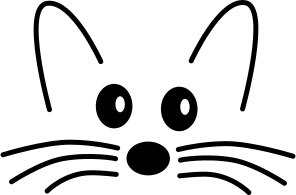
\includegraphics[width=1.4em]{squeak-logo}}}
\iftoshelse{
	\usepackage{marginnote}
		\renewcommand*{\marginfont}{\footnotesize}
	\newcommand{\vartriangleout}{\ifthenelse{\isodd{\thepage}}{\vartriangleright}{\vartriangleleft}}
	\newcommand{\dothisicon}{\fcolorbox{blue!65}{white}{\highlight{$\vartriangleout$}}}
	\newcommand{\dothis}[1]{%
		\noindent\par\noindent
		{\reversemarginpar
			\marginnote{\fcolorbox{blue!65}{white}{\highlight{$\vartriangleout$}}}}
		%\MarginLabel{do this}
		\noindent\emph{#1}
		\nopagebreak}
}{
	\newcommand{\dothisicon}{\raisebox{-.5ex}{
\includegraphics[height=1.2em]{pharo}}}
	\newcommand{\dothis}[1]{%
		\medskip
		\noindent\dothisicon
		\ifx#1\empty\else\quad\emph{#1}\fi
		\par\smallskip\nopagebreak}
}
%===> NEW VERSION <===
% NB: To use this in an individual chapter, you must set:
%\graphicspath{{figures/} {../figures/}}
% at the head of the chapter.  Don't forget the final /
%=============================================================
%:Reader hints (hint)
%
% Indicates a non-obvious consequence 
\newcommand{\hint}[1]{\vspace{1ex}\noindent\fbox{\textsc{Hint}} \emph{#1}}
%=================================================================
% graphics for Morphic handles
\newcommand{\grabHandle}{\raisebox{-0.2ex}{
\includegraphics[width=1em]{blackHandle}}}
\newcommand{\moveHandle}{\raisebox{-0.2ex}{
\includegraphics[width=1em]{moveHandle}}}
\newcommand{\debugHandle}{\raisebox{-0.2ex}{
\includegraphics[width=1em]{debugHandle}}}
%=============================================================
%:Highlighting Important stuff (doublebox)
%
% From Seaside book ...
\newsavebox{\SavedText}
\newlength{\InnerBoxRule}\setlength{\InnerBoxRule}{.75\fboxrule}
\newlength{\OuterBoxRule}\setlength{\OuterBoxRule}{1.5\fboxrule}
\newlength{\BoxSeparation}\setlength{\BoxSeparation}{1.5\fboxrule}
\addtolength{\BoxSeparation}{.5pt}
\newlength{\SaveBoxSep}\setlength{\SaveBoxSep}{2\fboxsep}
%
\newenvironment{doublebox}{\begin{lrbox}{\SavedText}
    \begin{minipage}{.75\textwidth}}
    {\end{minipage}\end{lrbox}\begin{center}
    \setlength{\fboxsep}{\BoxSeparation}\setlength{\fboxrule}{\OuterBoxRule}
    \fbox{\setlength{\fboxsep}{\SaveBoxSep}\setlength{\fboxrule}{\InnerBoxRule}%
      \fbox{\usebox{\SavedText}}}
  \end{center}}
% Use this:
\newcommand{\important}[1]{\begin{doublebox}#1\end{doublebox}}
%=============================================================
%:Section depth
\setcounter{secnumdepth}{2}
%% for this to happen start the file with
%\ifx\wholebook\relax\else
%% $Author$
% $Date$
% $Revision$

% HISTORY:
% 2006-10-31 - Oscar code macros
% ...

%=============================================================
% NB: documentclass must be set in main document.
% Allows book to be generated in multiple formats.
%=============================================================
%:Packages
\usepackage[T1]{fontenc}  %%%%%% really important to get the code directly in the text!
\usepackage{lmodern}
%\usepackage[scaled=0.85]{bookmanx} % needs another scale factor if used with \renewcommand{\sfdefault}{cmbr}
\usepackage{palatino}
\usepackage[scaled=0.85]{helvet}
\usepackage[protrusion,expansion=false]{microtype}
\usepackage{graphicx}
\usepackage{theorem}
\usepackage[english]{babel}
%%% ON: pdfsync breaks the use of p{width} for tabular columns!
%%\ifdefined\usepdfsync\usepackage{pdfsync}\fi % Requires texlive 2007
%=============================================================
%:More packages
%Stef should check which ones are used!
%\usepackage{picinpar}
%\usepackage{layout}
%\usepackage{color}
%\usepackage{enum}
%\usepackage{a4wide}
% \usepackage{fancyhdr}
\usepackage{ifthen}
\usepackage{float}
\usepackage{longtable}
\usepackage{makeidx}
\usepackage[nottoc]{tocbibind}
\usepackage{multicol}
\usepackage{booktabs}	% book-style tables
\usepackage{topcapt}	% enables \topcaption
\usepackage{multirow}
\usepackage{tabularx}
%\usepackage[bottom]{footmisc}
\usepackage{xspace}
\usepackage{alltt}
\usepackage{amssymb,textcomp}
\usepackage[usenames,dvipsnames]{color}
%\usepackage{colortbl}
\usepackage[hang]{subfigure}\makeatletter\def\p@subfigure{\thefigure\,}\makeatother
\usepackage{rotating}
\usepackage{enumitem}	% apb: allows more control over tags in enumerations
\usepackage{verbatim}     % for comment environment
\usepackage{varioref}	% for page references that work
\labelformat{footnote}{\thechapter--#1} % to distinguish citations from jurabib
\usepackage{needspace}
\usepackage{isodateo} % enable \isodate
\usepackage[newparttoc]{titlesec}
\usepackage{titletoc}
\usepackage{wrapfig}
\usepackage[
	super,
	citefull=first,
	authorformat={allreversed,and},
	titleformat={commasep,italic}
]{jurabib} % citations as footnotes
\usepackage[
	colorlinks=true,
	linkcolor=black,
	urlcolor=black,
	citecolor=black
]{hyperref}   % should come last
%=============================================================
%:PDF version
%%\pdfminorversion=3 % Set PDF to 1.3 for Lulu
%=============================================================
%:URL style
\makeatletter
\def\url@leostyle{%
  \@ifundefined{selectfont}{\def\UrlFont{\sf}}{\def\UrlFont{\sffamily}}}
\makeatother
% Now actually use the newly defined style.
\urlstyle{leo}
%=============================================================
%:Booleans
\newboolean{lulu}
\setboolean{lulu}{false}
\newcommand{\ifluluelse}[2]{\ifthenelse{\boolean{lulu}}{#1}{#2}}
%=============================================================
%:Names
\newcommand{\SUnit}{SUnit\xspace}
\newcommand{\sunit}{SUnit\xspace}
\newcommand{\xUnit}{$x$Unit\xspace}
\newcommand{\JUnit}{JUnit\xspace}
\newcommand{\st}{Smalltalk\xspace}
\newcommand{\pharo}{Pharo\xspace} % Use this, not \Pharo
%\newcommand{\sqmap}{SqueakMap\xspace}
\newcommand{\squeak}{Squeak\xspace} % use this, not \Squeak or \sq
\newcommand{\sqsrc}{SqueakSource\xspace}
\newcommand{\sbe}{\url{http://SqueakByExample.org}\xspace}
\newcommand{\pharoweb}{\url{http://pharo-project.org}\xspace}
\newcommand{\pbe}{\url{http://PharoByExample.org}\xspace}
\newcommand{\sba}{\url{http://SquareBracketAssociates.org}\xspace}
\newcommand{\bam}{\lct{Bounc\-ing\-Atoms\-Morph}\xspace}
%=============================================================
%:Markup macros for proof-reading
\usepackage[normalem]{ulem} % for \sout
\usepackage{xcolor}
\newcommand{\ra}{$\rightarrow$}
\newcommand{\ugh}[1]{\textcolor{red}{\uwave{#1}}} % please rephrase
\newcommand{\ins}[1]{\textcolor{blue}{\uline{#1}}} % please insert
\newcommand{\del}[1]{\textcolor{red}{\sout{#1}}} % please delete
\newcommand{\chg}[2]{\textcolor{red}{\sout{#1}}{\ra}\textcolor{blue}{\uline{#2}}} % please change
%=============================================================
%:Editorial comment macros
%\newcommand{\nnbb}[2]{
%    % \fbox{\bfseries\sffamily\scriptsize#1}
%    \fcolorbox{gray}{yellow}{\bfseries\sffamily\scriptsize#1}
%    {\sf\small$\blacktriangleright$\textit{#2}$\blacktriangleleft$}
%   }
\newcommand{\yellowbox}[1]{\fcolorbox{gray}{yellow}{\bfseries\sffamily\scriptsize#1}}
\newcommand{\triangles}[1]{{\sf\small$\blacktriangleright$\textit{#1}$\blacktriangleleft$}}
\newcommand{\nnbb}[2]{\yellowbox{#1} \triangles{#2}}
\newcommand{\fix}{\yellowbox{FIX!}}
\newcommand{\here}{\yellowbox{CONTINUE HERE!}}
% editor macros
\newcommand{\apl}[1]{\nnbb{Alain}{#1}} % Alain
\newcommand{\ab}[1]{\nnbb{Andrew}{#1}} % Black
\newcommand{\sd}[1]{\nnbb{St\'{e}f}{#1}} % Ducasse
\newcommand{\dc}[1]{\nnbb{DamienC}{#1}} % Ducasse
\newcommand{\md}[1]{\nnbb{Marcus}{#1}} % Denker
\newcommand{\on}[1]{\nnbb{Oscar}{#1}} % Nierstrasz
\newcommand{\damien}[1]{\nnbb{Damien}{#1}} % Pollet
\newcommand{\lr}[1]{\nnbb{Lukas}{#1}} % Renggli
\newcommand{\orla}[1]{\nnbb{Orla}{#1}} % Greevy
\newcommand{\alex}[1]{\nnbb{Alex}{#1}} % Bergel
\newcommand{\alx}[1]{\nnbb{Alex}{#1}} % Bergel
\newcommand{\dr}[1]{\nnbb{David}{#1}} % Roethlisberger
\newcommand{\ja}[1]{\nnbb{Jannik}{#1}} % Laval
\newcommand{\jr}[1]{\nnbb{Jorge}{#1}} % Ressia
\newcommand{\fp}[1]{\nnbb{Fabrizio}{#1}} % Perin
\newcommand{\michael}[1]{\nnbb{Michael}{#1}} % Davies
\newcommand{\ew}[1]{\nnbb{Erwann}{#1}} % Wernli
\newcommand{\mb}[1]{\nnbb{Martial}{#1}} % Boniou
\newcommand{\hw}[1]{\nnbb{Hernan}{#1}} % Wilkinson
%=============================================================
%:Abbreviation macros
\newcommand{\ie}{\emph{すなわち}、}
\newcommand{\eg}{\emph{例えば}、}
\newcommand{\etc}{などなど。}
%=============================================================
%:Cross reference macros
\newcommand{\charef}[1]{第~\ref{cha:#1}~章}
\newcommand{\secref}[1]{\ref{sec:#1}~節}
\newcommand{\figref}[1]{図~\ref{fig:#1}\xspace}
\newcommand{\Figref}[1]{図~\ref{fig:#1}\xspace}
\newcommand{\appref}[1]{付録~\ref{app:#1}\xspace}
\newcommand{\tabref}[1]{表~\ref{tab:#1}\xspace}
\newcommand{\faqref}[1]{FAQ~\ref{faq:#1}, p.~\pageref{faq:#1}\xspace}
% APB: I removed trailing \xspace commands from these macros because
% \xspace mostly doesn't work.  If you want a space after your
% references, type one!
% ON: xspace has always worked just fine for me!  Please leave them in.
%
\newcommand{\ruleref}[1]{\ref{rule:#1}\xspace}
%
\newcommand{\egref}[1]{example~\ref{eg:#1}\xspace}
\newcommand{\Egref}[1]{Example~\ref{eg:#1}\xspace}
%
\newcommand{\scrref}[1]{script~\ref{scr:#1}\xspace}
\newcommand{\Scrref}[1]{Script~\ref{scr:#1}\xspace}
\newcommand{\tscrref}[1]{the script~\ref{scr:#1}\xspace}
\newcommand{\Tscrref}[1]{The script~\ref{scr:#1}\xspace}
%
\newcommand{\mthref}[1]{method~\ref{mth:#1}\xspace}
\newcommand{\mthsref}[1]{methods~\ref{mth:#1}\xspace}
\newcommand{\Mthref}[1]{Method~\ref{mth:#1}\xspace}
\newcommand{\tmthref}[1]{the method~\ref{mth:#1}\xspace}
\newcommand{\Tmthref}[1]{The method~\ref{mth:#1}\xspace}
%
\newcommand{\clsref}[1]{class~\ref{cls:#1}\xspace}
\newcommand{\tclsref}[1]{the class~\ref{cls:#1}\xspace}
\newcommand{\Tclsref}[1]{The class~\ref{cls:#1}\xspace}

\newcommand{\chalabel}[1]{\label{cha:#1}}
\newcommand{\seclabel}[1]{\label{sec:#1}}
\newcommand{\figlabel}[1]{\label{fig:#1}}
\newcommand{\tablabel}[1]{\label{tab:#1}}
\newcommand{\rulelabel}[1]{\label{rule:#1}}
\newcommand{\eglabel}[1]{\label{eg:#1}}
\newcommand{\scrlabel}[1]{\label{scr:#1}}
\newcommand{\mthlabel}[1]{\label{mth:#1}}
\newcommand{\clslabel}[1]{\label{cls:#1}}
\newcommand{\faqlabel}[1]{\label{faq:#1}}
%=============================================================
%:Menu item macro
% for menu items, so we can change our minds on how to print them! (apb)
\definecolor{lightgray}{gray}{0.89}
\newcommand{\menu}[1]{{%
	\setlength{\fboxsep}{0pt}%
	\colorbox{lightgray}{{{\upshape\sffamily\strut \,#1\,}}}}}
\newcommand{\link}[1]{{%
	\fontfamily{lmr}\selectfont
 	\upshape{\sffamily \underline{#1}}}}
% For submenu items:
\newcommand{\go}{\,$\triangleright$\,}
% \newcommand{\go}{\,$\blacktriangleright$\,}
% For keyboard shortcuts:
%\newcommand{\short}[1]{\mbox{$\langle${\sc CMD}$\rangle$-#1}\xspace}
\newcommand{\short}[1]{\mbox{{\sc cmd}\hspace{0.08em}--\hspace{0.09em}#1}\xspace}
% For buttons:
\newcommand{\button}[1]{{%
	\setlength{\fboxsep}{0pt}%
	\fbox{{\upshape\sffamily\strut \,#1\,}}}}
% NB: The button macro does not work within captions -- incompatible with xcolor package :-(
\newcommand{\toolsflap}{\textit{Tools} flap\xspace}
%=============================================================
%:Mouse clicks
\newcommand{\click}{click\xspace} % RED
\newcommand{\actclick}{action-click\xspace} % YELLOW
\newcommand{\metaclick}{meta-click\xspace} % BLUE
\newcommand{\Click}{Click\xspace} % RED
\newcommand{\Actclick}{Action-click\xspace} % YELLOW
\newcommand{\Metaclick}{Meta-click\xspace} % BLUE
%=============================================================
%:ToSh macros
\newboolean{tosh}
\setboolean{tosh}{false}
\newcommand{\iftoshelse}[2]{\ifthenelse{\boolean{tosh}}{#1}{#2}}
%=============================================================
%:ToSh colors
%\newcommand{\highlightcolor}{\color{blue!65}}
%\newcommand{\boxcolor}{\color{gray!25}}
\newcommand{\highlight}[1]{\textcolor{blue!65}{#1}}
%\newcommand{\codecolor}{\color{blue!65}}
%%\setlength{\fboxrule}{2pt}
%\newcommand{\asPict}[1]{%
%	{\Large\highlight{#1}}}
%=============================================================
%:Reader cues (do this)
%
% Indicate something the reader should try out.
% \newcommand{\dothisicon}{\raisebox{-.5ex}{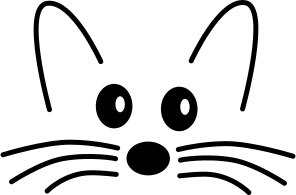
\includegraphics[width=1.4em]{squeak-logo}}}
\iftoshelse{
	\usepackage{marginnote}
		\renewcommand*{\marginfont}{\footnotesize}
	\newcommand{\vartriangleout}{\ifthenelse{\isodd{\thepage}}{\vartriangleright}{\vartriangleleft}}
	\newcommand{\dothisicon}{\fcolorbox{blue!65}{white}{\highlight{$\vartriangleout$}}}
	\newcommand{\dothis}[1]{%
		\noindent\par\noindent
		{\reversemarginpar
			\marginnote{\fcolorbox{blue!65}{white}{\highlight{$\vartriangleout$}}}}
		%\MarginLabel{do this}
		\noindent\emph{#1}
		\nopagebreak}
}{
	\newcommand{\dothisicon}{\raisebox{-.5ex}{
\includegraphics[height=1.2em]{pharo}}}
	\newcommand{\dothis}[1]{%
		\medskip
		\noindent\dothisicon
		\ifx#1\empty\else\quad\emph{#1}\fi
		\par\smallskip\nopagebreak}
}
%===> NEW VERSION <===
% NB: To use this in an individual chapter, you must set:
%\graphicspath{{figures/} {../figures/}}
% at the head of the chapter.  Don't forget the final /
%=============================================================
%:Reader hints (hint)
%
% Indicates a non-obvious consequence 
\newcommand{\hint}[1]{\vspace{1ex}\noindent\fbox{\textsc{Hint}} \emph{#1}}
%=================================================================
% graphics for Morphic handles
\newcommand{\grabHandle}{\raisebox{-0.2ex}{
\includegraphics[width=1em]{blackHandle}}}
\newcommand{\moveHandle}{\raisebox{-0.2ex}{
\includegraphics[width=1em]{moveHandle}}}
\newcommand{\debugHandle}{\raisebox{-0.2ex}{
\includegraphics[width=1em]{debugHandle}}}
%=============================================================
%:Highlighting Important stuff (doublebox)
%
% From Seaside book ...
\newsavebox{\SavedText}
\newlength{\InnerBoxRule}\setlength{\InnerBoxRule}{.75\fboxrule}
\newlength{\OuterBoxRule}\setlength{\OuterBoxRule}{1.5\fboxrule}
\newlength{\BoxSeparation}\setlength{\BoxSeparation}{1.5\fboxrule}
\addtolength{\BoxSeparation}{.5pt}
\newlength{\SaveBoxSep}\setlength{\SaveBoxSep}{2\fboxsep}
%
\newenvironment{doublebox}{\begin{lrbox}{\SavedText}
    \begin{minipage}{.75\textwidth}}
    {\end{minipage}\end{lrbox}\begin{center}
    \setlength{\fboxsep}{\BoxSeparation}\setlength{\fboxrule}{\OuterBoxRule}
    \fbox{\setlength{\fboxsep}{\SaveBoxSep}\setlength{\fboxrule}{\InnerBoxRule}%
      \fbox{\usebox{\SavedText}}}
  \end{center}}
% Use this:
\newcommand{\important}[1]{\begin{doublebox}#1\end{doublebox}}
%=============================================================
%:Section depth
\setcounter{secnumdepth}{2}
%% for this to happen start the file with
%\ifx\wholebook\relax\else
%% $Author$
% $Date$
% $Revision$

% HISTORY:
% 2006-10-31 - Oscar code macros
% ...

%=============================================================
% NB: documentclass must be set in main document.
% Allows book to be generated in multiple formats.
%=============================================================
%:Packages
\usepackage[T1]{fontenc}  %%%%%% really important to get the code directly in the text!
\usepackage{lmodern}
%\usepackage[scaled=0.85]{bookmanx} % needs another scale factor if used with \renewcommand{\sfdefault}{cmbr}
\usepackage{palatino}
\usepackage[scaled=0.85]{helvet}
\usepackage[protrusion,expansion=false]{microtype}
\usepackage{graphicx}
\usepackage{theorem}
\usepackage[english]{babel}
%%% ON: pdfsync breaks the use of p{width} for tabular columns!
%%\ifdefined\usepdfsync\usepackage{pdfsync}\fi % Requires texlive 2007
%=============================================================
%:More packages
%Stef should check which ones are used!
%\usepackage{picinpar}
%\usepackage{layout}
%\usepackage{color}
%\usepackage{enum}
%\usepackage{a4wide}
% \usepackage{fancyhdr}
\usepackage{ifthen}
\usepackage{float}
\usepackage{longtable}
\usepackage{makeidx}
\usepackage[nottoc]{tocbibind}
\usepackage{multicol}
\usepackage{booktabs}	% book-style tables
\usepackage{topcapt}	% enables \topcaption
\usepackage{multirow}
\usepackage{tabularx}
%\usepackage[bottom]{footmisc}
\usepackage{xspace}
\usepackage{alltt}
\usepackage{amssymb,textcomp}
\usepackage[usenames,dvipsnames]{color}
%\usepackage{colortbl}
\usepackage[hang]{subfigure}\makeatletter\def\p@subfigure{\thefigure\,}\makeatother
\usepackage{rotating}
\usepackage{enumitem}	% apb: allows more control over tags in enumerations
\usepackage{verbatim}     % for comment environment
\usepackage{varioref}	% for page references that work
\labelformat{footnote}{\thechapter--#1} % to distinguish citations from jurabib
\usepackage{needspace}
\usepackage{isodateo} % enable \isodate
\usepackage[newparttoc]{titlesec}
\usepackage{titletoc}
\usepackage{wrapfig}
\usepackage[
	super,
	citefull=first,
	authorformat={allreversed,and},
	titleformat={commasep,italic}
]{jurabib} % citations as footnotes
\usepackage[
	colorlinks=true,
	linkcolor=black,
	urlcolor=black,
	citecolor=black
]{hyperref}   % should come last
%=============================================================
%:PDF version
%%\pdfminorversion=3 % Set PDF to 1.3 for Lulu
%=============================================================
%:URL style
\makeatletter
\def\url@leostyle{%
  \@ifundefined{selectfont}{\def\UrlFont{\sf}}{\def\UrlFont{\sffamily}}}
\makeatother
% Now actually use the newly defined style.
\urlstyle{leo}
%=============================================================
%:Booleans
\newboolean{lulu}
\setboolean{lulu}{false}
\newcommand{\ifluluelse}[2]{\ifthenelse{\boolean{lulu}}{#1}{#2}}
%=============================================================
%:Names
\newcommand{\SUnit}{SUnit\xspace}
\newcommand{\sunit}{SUnit\xspace}
\newcommand{\xUnit}{$x$Unit\xspace}
\newcommand{\JUnit}{JUnit\xspace}
\newcommand{\st}{Smalltalk\xspace}
\newcommand{\pharo}{Pharo\xspace} % Use this, not \Pharo
%\newcommand{\sqmap}{SqueakMap\xspace}
\newcommand{\squeak}{Squeak\xspace} % use this, not \Squeak or \sq
\newcommand{\sqsrc}{SqueakSource\xspace}
\newcommand{\sbe}{\url{http://SqueakByExample.org}\xspace}
\newcommand{\pharoweb}{\url{http://pharo-project.org}\xspace}
\newcommand{\pbe}{\url{http://PharoByExample.org}\xspace}
\newcommand{\sba}{\url{http://SquareBracketAssociates.org}\xspace}
\newcommand{\bam}{\lct{Bounc\-ing\-Atoms\-Morph}\xspace}
%=============================================================
%:Markup macros for proof-reading
\usepackage[normalem]{ulem} % for \sout
\usepackage{xcolor}
\newcommand{\ra}{$\rightarrow$}
\newcommand{\ugh}[1]{\textcolor{red}{\uwave{#1}}} % please rephrase
\newcommand{\ins}[1]{\textcolor{blue}{\uline{#1}}} % please insert
\newcommand{\del}[1]{\textcolor{red}{\sout{#1}}} % please delete
\newcommand{\chg}[2]{\textcolor{red}{\sout{#1}}{\ra}\textcolor{blue}{\uline{#2}}} % please change
%=============================================================
%:Editorial comment macros
%\newcommand{\nnbb}[2]{
%    % \fbox{\bfseries\sffamily\scriptsize#1}
%    \fcolorbox{gray}{yellow}{\bfseries\sffamily\scriptsize#1}
%    {\sf\small$\blacktriangleright$\textit{#2}$\blacktriangleleft$}
%   }
\newcommand{\yellowbox}[1]{\fcolorbox{gray}{yellow}{\bfseries\sffamily\scriptsize#1}}
\newcommand{\triangles}[1]{{\sf\small$\blacktriangleright$\textit{#1}$\blacktriangleleft$}}
\newcommand{\nnbb}[2]{\yellowbox{#1} \triangles{#2}}
\newcommand{\fix}{\yellowbox{FIX!}}
\newcommand{\here}{\yellowbox{CONTINUE HERE!}}
% editor macros
\newcommand{\apl}[1]{\nnbb{Alain}{#1}} % Alain
\newcommand{\ab}[1]{\nnbb{Andrew}{#1}} % Black
\newcommand{\sd}[1]{\nnbb{St\'{e}f}{#1}} % Ducasse
\newcommand{\dc}[1]{\nnbb{DamienC}{#1}} % Ducasse
\newcommand{\md}[1]{\nnbb{Marcus}{#1}} % Denker
\newcommand{\on}[1]{\nnbb{Oscar}{#1}} % Nierstrasz
\newcommand{\damien}[1]{\nnbb{Damien}{#1}} % Pollet
\newcommand{\lr}[1]{\nnbb{Lukas}{#1}} % Renggli
\newcommand{\orla}[1]{\nnbb{Orla}{#1}} % Greevy
\newcommand{\alex}[1]{\nnbb{Alex}{#1}} % Bergel
\newcommand{\alx}[1]{\nnbb{Alex}{#1}} % Bergel
\newcommand{\dr}[1]{\nnbb{David}{#1}} % Roethlisberger
\newcommand{\ja}[1]{\nnbb{Jannik}{#1}} % Laval
\newcommand{\jr}[1]{\nnbb{Jorge}{#1}} % Ressia
\newcommand{\fp}[1]{\nnbb{Fabrizio}{#1}} % Perin
\newcommand{\michael}[1]{\nnbb{Michael}{#1}} % Davies
\newcommand{\ew}[1]{\nnbb{Erwann}{#1}} % Wernli
\newcommand{\mb}[1]{\nnbb{Martial}{#1}} % Boniou
\newcommand{\hw}[1]{\nnbb{Hernan}{#1}} % Wilkinson
%=============================================================
%:Abbreviation macros
\newcommand{\ie}{\emph{すなわち}、}
\newcommand{\eg}{\emph{例えば}、}
\newcommand{\etc}{などなど。}
%=============================================================
%:Cross reference macros
\newcommand{\charef}[1]{第~\ref{cha:#1}~章}
\newcommand{\secref}[1]{\ref{sec:#1}~節}
\newcommand{\figref}[1]{図~\ref{fig:#1}\xspace}
\newcommand{\Figref}[1]{図~\ref{fig:#1}\xspace}
\newcommand{\appref}[1]{付録~\ref{app:#1}\xspace}
\newcommand{\tabref}[1]{表~\ref{tab:#1}\xspace}
\newcommand{\faqref}[1]{FAQ~\ref{faq:#1}, p.~\pageref{faq:#1}\xspace}
% APB: I removed trailing \xspace commands from these macros because
% \xspace mostly doesn't work.  If you want a space after your
% references, type one!
% ON: xspace has always worked just fine for me!  Please leave them in.
%
\newcommand{\ruleref}[1]{\ref{rule:#1}\xspace}
%
\newcommand{\egref}[1]{example~\ref{eg:#1}\xspace}
\newcommand{\Egref}[1]{Example~\ref{eg:#1}\xspace}
%
\newcommand{\scrref}[1]{script~\ref{scr:#1}\xspace}
\newcommand{\Scrref}[1]{Script~\ref{scr:#1}\xspace}
\newcommand{\tscrref}[1]{the script~\ref{scr:#1}\xspace}
\newcommand{\Tscrref}[1]{The script~\ref{scr:#1}\xspace}
%
\newcommand{\mthref}[1]{method~\ref{mth:#1}\xspace}
\newcommand{\mthsref}[1]{methods~\ref{mth:#1}\xspace}
\newcommand{\Mthref}[1]{Method~\ref{mth:#1}\xspace}
\newcommand{\tmthref}[1]{the method~\ref{mth:#1}\xspace}
\newcommand{\Tmthref}[1]{The method~\ref{mth:#1}\xspace}
%
\newcommand{\clsref}[1]{class~\ref{cls:#1}\xspace}
\newcommand{\tclsref}[1]{the class~\ref{cls:#1}\xspace}
\newcommand{\Tclsref}[1]{The class~\ref{cls:#1}\xspace}

\newcommand{\chalabel}[1]{\label{cha:#1}}
\newcommand{\seclabel}[1]{\label{sec:#1}}
\newcommand{\figlabel}[1]{\label{fig:#1}}
\newcommand{\tablabel}[1]{\label{tab:#1}}
\newcommand{\rulelabel}[1]{\label{rule:#1}}
\newcommand{\eglabel}[1]{\label{eg:#1}}
\newcommand{\scrlabel}[1]{\label{scr:#1}}
\newcommand{\mthlabel}[1]{\label{mth:#1}}
\newcommand{\clslabel}[1]{\label{cls:#1}}
\newcommand{\faqlabel}[1]{\label{faq:#1}}
%=============================================================
%:Menu item macro
% for menu items, so we can change our minds on how to print them! (apb)
\definecolor{lightgray}{gray}{0.89}
\newcommand{\menu}[1]{{%
	\setlength{\fboxsep}{0pt}%
	\colorbox{lightgray}{{{\upshape\sffamily\strut \,#1\,}}}}}
\newcommand{\link}[1]{{%
	\fontfamily{lmr}\selectfont
 	\upshape{\sffamily \underline{#1}}}}
% For submenu items:
\newcommand{\go}{\,$\triangleright$\,}
% \newcommand{\go}{\,$\blacktriangleright$\,}
% For keyboard shortcuts:
%\newcommand{\short}[1]{\mbox{$\langle${\sc CMD}$\rangle$-#1}\xspace}
\newcommand{\short}[1]{\mbox{{\sc cmd}\hspace{0.08em}--\hspace{0.09em}#1}\xspace}
% For buttons:
\newcommand{\button}[1]{{%
	\setlength{\fboxsep}{0pt}%
	\fbox{{\upshape\sffamily\strut \,#1\,}}}}
% NB: The button macro does not work within captions -- incompatible with xcolor package :-(
\newcommand{\toolsflap}{\textit{Tools} flap\xspace}
%=============================================================
%:Mouse clicks
\newcommand{\click}{click\xspace} % RED
\newcommand{\actclick}{action-click\xspace} % YELLOW
\newcommand{\metaclick}{meta-click\xspace} % BLUE
\newcommand{\Click}{Click\xspace} % RED
\newcommand{\Actclick}{Action-click\xspace} % YELLOW
\newcommand{\Metaclick}{Meta-click\xspace} % BLUE
%=============================================================
%:ToSh macros
\newboolean{tosh}
\setboolean{tosh}{false}
\newcommand{\iftoshelse}[2]{\ifthenelse{\boolean{tosh}}{#1}{#2}}
%=============================================================
%:ToSh colors
%\newcommand{\highlightcolor}{\color{blue!65}}
%\newcommand{\boxcolor}{\color{gray!25}}
\newcommand{\highlight}[1]{\textcolor{blue!65}{#1}}
%\newcommand{\codecolor}{\color{blue!65}}
%%\setlength{\fboxrule}{2pt}
%\newcommand{\asPict}[1]{%
%	{\Large\highlight{#1}}}
%=============================================================
%:Reader cues (do this)
%
% Indicate something the reader should try out.
% \newcommand{\dothisicon}{\raisebox{-.5ex}{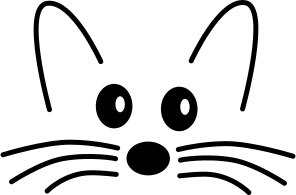
\includegraphics[width=1.4em]{squeak-logo}}}
\iftoshelse{
	\usepackage{marginnote}
		\renewcommand*{\marginfont}{\footnotesize}
	\newcommand{\vartriangleout}{\ifthenelse{\isodd{\thepage}}{\vartriangleright}{\vartriangleleft}}
	\newcommand{\dothisicon}{\fcolorbox{blue!65}{white}{\highlight{$\vartriangleout$}}}
	\newcommand{\dothis}[1]{%
		\noindent\par\noindent
		{\reversemarginpar
			\marginnote{\fcolorbox{blue!65}{white}{\highlight{$\vartriangleout$}}}}
		%\MarginLabel{do this}
		\noindent\emph{#1}
		\nopagebreak}
}{
	\newcommand{\dothisicon}{\raisebox{-.5ex}{
\includegraphics[height=1.2em]{pharo}}}
	\newcommand{\dothis}[1]{%
		\medskip
		\noindent\dothisicon
		\ifx#1\empty\else\quad\emph{#1}\fi
		\par\smallskip\nopagebreak}
}
%===> NEW VERSION <===
% NB: To use this in an individual chapter, you must set:
%\graphicspath{{figures/} {../figures/}}
% at the head of the chapter.  Don't forget the final /
%=============================================================
%:Reader hints (hint)
%
% Indicates a non-obvious consequence 
\newcommand{\hint}[1]{\vspace{1ex}\noindent\fbox{\textsc{Hint}} \emph{#1}}
%=================================================================
% graphics for Morphic handles
\newcommand{\grabHandle}{\raisebox{-0.2ex}{
\includegraphics[width=1em]{blackHandle}}}
\newcommand{\moveHandle}{\raisebox{-0.2ex}{
\includegraphics[width=1em]{moveHandle}}}
\newcommand{\debugHandle}{\raisebox{-0.2ex}{
\includegraphics[width=1em]{debugHandle}}}
%=============================================================
%:Highlighting Important stuff (doublebox)
%
% From Seaside book ...
\newsavebox{\SavedText}
\newlength{\InnerBoxRule}\setlength{\InnerBoxRule}{.75\fboxrule}
\newlength{\OuterBoxRule}\setlength{\OuterBoxRule}{1.5\fboxrule}
\newlength{\BoxSeparation}\setlength{\BoxSeparation}{1.5\fboxrule}
\addtolength{\BoxSeparation}{.5pt}
\newlength{\SaveBoxSep}\setlength{\SaveBoxSep}{2\fboxsep}
%
\newenvironment{doublebox}{\begin{lrbox}{\SavedText}
    \begin{minipage}{.75\textwidth}}
    {\end{minipage}\end{lrbox}\begin{center}
    \setlength{\fboxsep}{\BoxSeparation}\setlength{\fboxrule}{\OuterBoxRule}
    \fbox{\setlength{\fboxsep}{\SaveBoxSep}\setlength{\fboxrule}{\InnerBoxRule}%
      \fbox{\usebox{\SavedText}}}
  \end{center}}
% Use this:
\newcommand{\important}[1]{\begin{doublebox}#1\end{doublebox}}
%=============================================================
%:Section depth
\setcounter{secnumdepth}{2}
%% for this to happen start the file with
%\ifx\wholebook\relax\else
%\input{../common.tex}
%\begin{document}
%\fi
% and terminate by
% \ifx\wholebook\relax\else\end{document}\fi

\DeclareGraphicsExtensions{.pdf, .jpg, .png}
%=============================================================
%:PDF setup
\hypersetup{
%   a4paper,
%   pdfstartview=FitV,
%   colorlinks,
%   linkcolor=darkblue,
%   citecolor=darkblue,
   pdftitle={Pharo by Example},
   pdfauthor={Andrew P. Black, St\'ephane Ducasse,	Oscar Nierstrasz,
Damien Pollet},
   pdfkeywords={Smalltalk, Squeak, Object-Oriented Programming, OOP},
   pdfsubject={Computer Science}
}
%=============================================================
%:Page layout and appearance
%
% \renewcommand{\headrulewidth}{0pt}
\renewcommand{\chaptermark}[1]{\markboth{#1}{}}
\renewcommand{\sectionmark}[1]{\markright{\thesection\ #1}}
\renewpagestyle{plain}[\small\itshape]{%
	\setheadrule{0pt}%
	\sethead[][][]{}{}{}%
	\setfoot[][][]{}{}{}}
\renewpagestyle{headings}[\small\itshape]{%
	\setheadrule{0pt}%
	\setmarks{chapter}{section}%
	\sethead[\thepage][][\chaptertitle]{\sectiontitle}{}{\thepage}%
	\setfoot[][][]{}{}{}}
%=============================================================
%:Title section setup and TOC numbering depth
\setcounter{secnumdepth}{1}
\setcounter{tocdepth}{1}
\titleformat{\part}[display]{\centering}{\huge\partname\ \thepart}{1em}{\Huge\textbf}[]
\titleformat{\chapter}[display]{}{\huge\chaptertitlename\ \thechapter}{1em}{\Huge\raggedright\textbf}[]
\titlecontents{part}[3pc]{%
		\pagebreak[2]\addvspace{1em plus.4em minus.2em}%
		\leavevmode\large\bfseries}
	{\contentslabel{3pc}}{\hspace*{-3pc}}
	{}[\nopagebreak]
\titlecontents{chapter}[3pc]{%
		\pagebreak[0]\addvspace{1em plus.2em minus.2em}%
		\leavevmode\bfseries}
	{\contentslabel{3pc}}{}
	{\hfill\contentspage}[\nopagebreak]
\dottedcontents{section}[3pc]{}{3pc}{1pc}
\dottedcontents{subsection}[3pc]{}{0pc}{1pc}
% \dottedcontents{subsection}[4.5em]{}{0pt}{1pc}
% Make \cleardoublepage insert really blank pages http://www.tex.ac.uk/cgi-bin/texfaq2html?label=reallyblank
\let\origdoublepage\cleardoublepage
\newcommand{\clearemptydoublepage}{%
  \clearpage
  {\pagestyle{empty}\origdoublepage}}
\let\cleardoublepage\clearemptydoublepage % see http://www.tex.ac.uk/cgi-bin/texfaq2html?label=patch
%=============================================================
%:FAQ macros (for FAQ chapter)
\newtheorem{faq}{FAQ}
\newcommand{\answer}{\paragraph{Answer}\ }
%=============================================================
%:Listings package configuration
% \newcommand{\caret}{\makebox{\raisebox{0.4ex}{\footnotesize{$\wedge$}}}}
\newcommand{\caret}{\^\,}
\newcommand{\escape}{{\sf \textbackslash}}
\definecolor{source}{gray}{0.95}
\usepackage{listings}
\lstdefinelanguage{Smalltalk}{
%  morekeywords={self,super,true,false,nil,thisContext}, % This is overkill
  morestring=[d]',
  morecomment=[s]{"}{"},
  alsoletter={\#:},
  escapechar={!},
  literate=
    {BANG}{!}1
    {CARET}{\^}1
    {UNDERSCORE}{\_}1
    {\\st}{Smalltalk}9 % convenience -- in case \st occurs in code
    % {'}{{\textquotesingle}}1 % replaced by upquote=true in \lstset
    {_}{{$\leftarrow$}}1
    {>>>}{{\sep}}1
    {^}{{$\uparrow$}}1
    {~}{{$\sim$}}1
    {-}{{\texttt{-}}}1 %{\textminus}}1 %{-}{\hspace{-0.13em}}{-}}1  % the goal is to make - the same width as +
    % {+}{\sf+}1 %{\raisebox{0.08ex}{+}}}1      % and to raise + off the baseline to match -
    {-->}{{\quad$\longrightarrow$\quad}}3
	, % Don't forget the comma at the end!
  tabsize=4
}[keywords,comments,strings]

\lstset{language=Smalltalk,
	basicstyle=\sffamily,
	keywordstyle=\color{black}\bfseries,
	% stringstyle=\ttfamily, % Ugly! do we really want this? -- on
	mathescape=true,
	showstringspaces=false,
	keepspaces=true,
	breaklines=true,
	breakautoindent=true,
	backgroundcolor=\color{source},
	lineskip={-1pt}, % Ugly hack
	upquote=true, % straight quote; requires textcomp package
	columns=fullflexible} % no fixed width fonts
% In-line code (literal)
% Normally use this for all in-line code:
\newcommand{\ct}{\lstinline[mathescape=false,backgroundcolor=\color{white},basicstyle={\sffamily\upshape}]}
% apb 2007.8.28 added the \upshape declaration to avoid getting italicized code in \dothis{ } sections.
% In-line code (latex enabled)
% Use this only in special situations where \ct does not work
% (within section headings ...):
\newcommand{\lct}[1]{{\textsf{\textup{#1}}}}
% Use these for system categories and protocols:
\newcommand{\scat}[1]{\emph{\textsf{#1}}\xspace}
\newcommand{\pkg}[1]{\emph{\textsf{#1}}\xspace}
\newcommand{\prot}[1]{\emph{\textsf{#1}}\xspace}
% Code environments
% NB: the arg is for tests
% Only code and example environments may be tests
\lstnewenvironment{code}[1]{%
	\lstset{%
		% frame=lines,
		frame=single,
		framerule=0pt,
		mathescape=false
	}
}{}
\def\ignoredollar#1{}
%=============================================================
%:Code environments (method, script ...)
% NB: the third arg is for tests
% Only code and example environments may be tests
\lstnewenvironment{example}[3][defaultlabel]{%
	\renewcommand{\lstlistingname}{Example}%
	\lstset{
		% frame=lines,
		frame=single,
		framerule=0pt,
		mathescape=false,
		caption={\emph{#2}},
		label={eg:#1}
	}
}{}
\lstnewenvironment{script}[2][defaultlabel]{%
\renewcommand{\lstlistingname}{Script}%
	\lstset{
		% frame=lines,
		frame=single,
		framerule=0pt,
		mathescape=false,
		name={Script},
		caption={\emph{#2}},
		label={scr:#1}
	}
}{}
\lstnewenvironment{method}[2][defaultlabel]{%
	\renewcommand{\lstlistingname}{Method}%
	\lstset{
		% frame=lines,
		frame=single,
		framerule=0pt,
		mathescape=false,
		name={Method},
		caption={\emph{#2}},
		label={mth:#1}
	}
}{}
\lstnewenvironment{methods}[2][defaultlabel]{% just for multiple methods at once
	\renewcommand{\lstlistingname}{Methods}%
	\lstset{
		% frame=lines,
		frame=single,
		framerule=0pt,
		mathescape=false,
		name={Method},
		caption={\emph{#2}},
		label={mth:#1}
	}
}{}
\lstnewenvironment{numMethod}[2][defaultlabel]{%
	\renewcommand{\lstlistingname}{Method}%
	\lstset{
		numbers=left,
		numberstyle={\tiny\sffamily},
		% frame=lines,
		frame=single,
		framerule=0pt,
		mathescape=false,
		name={Method},
		caption={\emph{#2}},
		label={mth:#1}
	}
}{}
\lstnewenvironment{classdef}[2][defaultlabel]{%
	\renewcommand{\lstlistingname}{Class}%
	\lstset{
		% frame=lines,
		frame=single,
		framerule=0pt,
		mathescape=false,
		name={Class},
		caption={\emph{#2}},
		label={cls:#1}
	}
}{}
%=============================================================
%:Reserving space
% Usually need one more line than the actual lines of code
\newcommand{\needlines}[1]{\Needspace{#1\baselineskip}}
%=============================================================
%:Indexing macros
% Macros ending with "ind" generate text as well as an index entry
% Macros ending with "index" *only* generate an index entry
\newcommand{\ind}[1]{\index{#1}#1\xspace} % plain text
\newcommand{\subind}[2]{\index{#1!#2}#2\xspace} % show #2, subindex under #1
\newcommand{\emphind}[1]{\index{#1}\emph{#1}\xspace} % emph #1
\newcommand{\emphsubind}[2]{\index{#1!#2}\emph{#2}\xspace} % show emph #2, subindex inder #1
\newcommand{\scatind}[1]{\index{#1@\textsf{#1} (category)}\scat{#1}} % category
\newcommand{\pkgind}[1]{\index{#1@\textsf{#1} (package)}\pkg{#1}} % package
\newcommand{\protind}[1]{\index{#1@\textsf{#1} (protocol)}\prot{#1}} % protocol
\newcommand{\clsind}[1]{\index{#1@\textsf{#1} (class)}\ct{#1}\xspace}
% \newcommand{\clsind}[1]{\index{#1!\#@(class)}\ct{#1}\xspace} % class
\newcommand{\clsindplural}[1]{\index{#1!\#@(class)}\ct{#1}s\xspace} % class
\newcommand{\cvind}[1]{\index{#1@\textsf{#1} (class variable)}\ct{#1}\xspace} % class var
\newcommand{\glbind}[1]{\index{#1@\textsf{#1} (global)}\ct{#1}\xspace} % global
\newcommand{\patind}[1]{\index{#1@#1 (pattern)}\ct{#1}\xspace} % pattern
\newcommand{\pvind}[1]{\index{#1@\textsf{#1} (pseudo variable)}\ct{#1}\xspace} % pseudo var
\newcommand{\clsmthind}[2]{\index{#1!#2@\ct{#2}}\ct{#1>>>#2}\xspace} % class + method name
\newcommand{\mthind}[2]{\index{#1!#2@\ct{#2}}\ct{#2}\xspace} % show method name only
\newcommand{\lmthind}[2]{\index{#1!#2@\ct{#2}}\lct{#2}\xspace} % show method name only
\newcommand{\cmind}[2]{\index{#1!#2@\ct{#2}}\ct{#1>>>#2}\xspace} % show class>>method
\newcommand{\lcmind}[2]{\index{#1!#2@\ct{#2}}\lct{#1>>>#2}\xspace} % show class>>method
\newcommand{\toolsflapind}{\index{Tools flap}\toolsflap} % index tools flap
% The following only generate an index entry:
% \newcommand{\clsindex}[1]{\index{#1@\textsf{#1} (class)}}
\newcommand{\clsindex}[1]{\index{#1!\#@(class)}} % class
\newcommand{\mthindex}[2]{\index{#1!#2@\ct{#2}}} % method
\newcommand{\cmindex}[2]{\index{#1!#2@\ct{#2}}} % class>>method
\newcommand{\cvindex}[1]{\index{#1@\textsf{#1} (class variable)}} % class var
\newcommand{\glbindex}[1]{\index{#1@\textsf{#1} (global)}}% global
\newcommand{\pvindex}[1]{\index{#1@\textsf{#1} (pseudo variable)}}% pseudo var
\newcommand{\seeindex}[2]{\index{#1|see{#2}}} % #1, see #2
\newcommand{\scatindex}[1]{\index{#1@\textsf{#1} (category)}} % category
\newcommand{\pkgindex}[1]{\index{#1@\textsf{#1} (package)}} % package
\newcommand{\protindex}[1]{\index{#1@\textsf{#1} (protocol)}} % protocol
% How can we have the main entry page numbers in bold yet not break the hyperlink?
\newcommand{\boldidx}[1]{{\bf #1}} % breaks hyperlink
%\newcommand{\indmain}[1]{\index{#1|boldidx}#1\xspace} % plain text, main entry
%\newcommand{\emphsubindmain}[2]{\index{#1!#2|boldidx}\emph{#2}\xspace} % subindex, main entry
%\newcommand{\subindmain}[2]{\index{#1!#2|boldidx}#2\xspace} % subindex, main entry
%\newcommand{\clsindmain}[1]{\index{#1@\textsf{#1} (class)|boldidx}\ct{#1}\xspace}
%\newcommand{\clsindmain}[1]{\index{#1!\#@(class)|boldidx}\ct{#1}\xspace} % class main
%\newcommand{\indexmain}[1]{\index{#1|boldidx}} % main index entry only
\newcommand{\indmain}[1]{\index{#1}#1\xspace} % The main index entry for this item
\newcommand{\emphsubindmain}[2]{\index{#1!#2}\emph{#2}\xspace} % subindex, main entry
\newcommand{\subindmain}[2]{\index{#1!#2}#2\xspace} % subindex, main entry
%\newcommand{\clsindmain}[1]{\index{#1@\textsf{#1} (class)}\ct{#1}\xspace}
\newcommand{\clsindmain}[1]{\index{#1!\#@(class)}\ct{#1}\xspace} % class main
\newcommand{\clsindexmain}[1]{\index{#1!\#@(class)}} % class main index only
\newcommand{\indexmain}[1]{\index{#1}} 
%=============================================================
%:Code macros
% some constants
\newcommand{\codesize}{\small}
\newcommand{\codefont}{\sffamily}
%\newcommand{\cat}[1]{\textit{In category #1}}%%To remove later
\newlength{\scriptindent}
\setlength{\scriptindent}{.3cm}
%% Method presentation constants
\newlength{\methodindent}
\newlength{\methodwordlength}
\newlength{\aftermethod}
\setlength{\methodindent}{0.2cm}
\settowidth{\methodwordlength}{\ M\'ethode\ }
%=============================================================
%:Smalltalk macros
%\newcommand{\sep}{{$\gg$}}
\newcommand{\sep}{\mbox{>>}}
\newcommand{\self}{\lct{self}\xspace}
\newcommand{\super}{\lct{super}\xspace}
\newcommand{\nil}{\lct{nil}\xspace}
%=============================================================
% be less conservative about float placement
% these commands are from http://www.tex.ac.uk/cgi-bin/texfaq2html?label=floats
\renewcommand{\topfraction}{.9}
\renewcommand{\bottomfraction}{.9}
\renewcommand{\textfraction}{.1}
\renewcommand{\floatpagefraction}{.85}
\renewcommand{\dbltopfraction}{.66}
\renewcommand{\dblfloatpagefraction}{.85}
\setcounter{topnumber}{9}
\setcounter{bottomnumber}{9}
\setcounter{totalnumber}{20}
\setcounter{dbltopnumber}{9}
%=============================================================
% Give information from each chapter's author
\newcommand{\contact}[2]{\textbf{#1} \textsf{(#2)}}

\newcommand{\chapterauthor}[1]{\emph{with the participation of:\\#1}\\}

\newcommand{\authornoury}{\contact{Noury Bouraqadi}{bouraqadi@gmail.com}}
\newcommand{\authordamienc}{\contact{Damien Cassou}{damien.cassou@gmail.com}}
\newcommand{\authoroscar}{\contact{Oscar Nierstrasz}{oscar.nierstrasz@acm.org}}
\newcommand{\authorsteph}{\contact{St\'ephane Ducasse}{stephane.ducasse@inria.fr}}
\newcommand{\authoralex}{\contact{Alexandre Bergel}{alexandre@bergel.eu}}
\newcommand{\authorolivier}{\contact{Olivier Auverlot}{olivier.auverlot@inria.fr}}
\newcommand{\authornicolas}{\contact{Nicolas Cellier}{ncellier@ifrance.com}}
\newcommand{\authormarcus}{\contact{Marcus Denker}{marcus.denker@inria.fr}}
\newcommand{\authoralain}{\contact{Alain Plantec}{alain.plantec@univ-brest.fr}}
\newcommand{\authordale}{\contact{Dale Henrichs}{dale.henrichs@gemstone.com}}
\newcommand{\authormariano}{\contact{Mariano Martinez Peck}{marianopeck@gmail.com}}
\newcommand{\authorsven}{\contact{Sven Van Caekenberghe}{sven@beta9.be}}

%=============================================================
% apb doesn't like paragraphs to run in to each other without a break
\parskip 1ex
%=============================================================
%:Stuff to check, merge or deprecate
%\setlength{\marginparsep}{2mm}
%\renewcommand{\baselinestretch}{1.1}
%=============================================================

%\begin{document}
%\fi
% and terminate by
% \ifx\wholebook\relax\else\end{document}\fi

\DeclareGraphicsExtensions{.pdf, .jpg, .png}
%=============================================================
%:PDF setup
\hypersetup{
%   a4paper,
%   pdfstartview=FitV,
%   colorlinks,
%   linkcolor=darkblue,
%   citecolor=darkblue,
   pdftitle={Pharo by Example},
   pdfauthor={Andrew P. Black, St\'ephane Ducasse,	Oscar Nierstrasz,
Damien Pollet},
   pdfkeywords={Smalltalk, Squeak, Object-Oriented Programming, OOP},
   pdfsubject={Computer Science}
}
%=============================================================
%:Page layout and appearance
%
% \renewcommand{\headrulewidth}{0pt}
\renewcommand{\chaptermark}[1]{\markboth{#1}{}}
\renewcommand{\sectionmark}[1]{\markright{\thesection\ #1}}
\renewpagestyle{plain}[\small\itshape]{%
	\setheadrule{0pt}%
	\sethead[][][]{}{}{}%
	\setfoot[][][]{}{}{}}
\renewpagestyle{headings}[\small\itshape]{%
	\setheadrule{0pt}%
	\setmarks{chapter}{section}%
	\sethead[\thepage][][\chaptertitle]{\sectiontitle}{}{\thepage}%
	\setfoot[][][]{}{}{}}
%=============================================================
%:Title section setup and TOC numbering depth
\setcounter{secnumdepth}{1}
\setcounter{tocdepth}{1}
\titleformat{\part}[display]{\centering}{\huge\partname\ \thepart}{1em}{\Huge\textbf}[]
\titleformat{\chapter}[display]{}{\huge\chaptertitlename\ \thechapter}{1em}{\Huge\raggedright\textbf}[]
\titlecontents{part}[3pc]{%
		\pagebreak[2]\addvspace{1em plus.4em minus.2em}%
		\leavevmode\large\bfseries}
	{\contentslabel{3pc}}{\hspace*{-3pc}}
	{}[\nopagebreak]
\titlecontents{chapter}[3pc]{%
		\pagebreak[0]\addvspace{1em plus.2em minus.2em}%
		\leavevmode\bfseries}
	{\contentslabel{3pc}}{}
	{\hfill\contentspage}[\nopagebreak]
\dottedcontents{section}[3pc]{}{3pc}{1pc}
\dottedcontents{subsection}[3pc]{}{0pc}{1pc}
% \dottedcontents{subsection}[4.5em]{}{0pt}{1pc}
% Make \cleardoublepage insert really blank pages http://www.tex.ac.uk/cgi-bin/texfaq2html?label=reallyblank
\let\origdoublepage\cleardoublepage
\newcommand{\clearemptydoublepage}{%
  \clearpage
  {\pagestyle{empty}\origdoublepage}}
\let\cleardoublepage\clearemptydoublepage % see http://www.tex.ac.uk/cgi-bin/texfaq2html?label=patch
%=============================================================
%:FAQ macros (for FAQ chapter)
\newtheorem{faq}{FAQ}
\newcommand{\answer}{\paragraph{Answer}\ }
%=============================================================
%:Listings package configuration
% \newcommand{\caret}{\makebox{\raisebox{0.4ex}{\footnotesize{$\wedge$}}}}
\newcommand{\caret}{\^\,}
\newcommand{\escape}{{\sf \textbackslash}}
\definecolor{source}{gray}{0.95}
\usepackage{listings}
\lstdefinelanguage{Smalltalk}{
%  morekeywords={self,super,true,false,nil,thisContext}, % This is overkill
  morestring=[d]',
  morecomment=[s]{"}{"},
  alsoletter={\#:},
  escapechar={!},
  literate=
    {BANG}{!}1
    {CARET}{\^}1
    {UNDERSCORE}{\_}1
    {\\st}{Smalltalk}9 % convenience -- in case \st occurs in code
    % {'}{{\textquotesingle}}1 % replaced by upquote=true in \lstset
    {_}{{$\leftarrow$}}1
    {>>>}{{\sep}}1
    {^}{{$\uparrow$}}1
    {~}{{$\sim$}}1
    {-}{{\texttt{-}}}1 %{\textminus}}1 %{-}{\hspace{-0.13em}}{-}}1  % the goal is to make - the same width as +
    % {+}{\sf+}1 %{\raisebox{0.08ex}{+}}}1      % and to raise + off the baseline to match -
    {-->}{{\quad$\longrightarrow$\quad}}3
	, % Don't forget the comma at the end!
  tabsize=4
}[keywords,comments,strings]

\lstset{language=Smalltalk,
	basicstyle=\sffamily,
	keywordstyle=\color{black}\bfseries,
	% stringstyle=\ttfamily, % Ugly! do we really want this? -- on
	mathescape=true,
	showstringspaces=false,
	keepspaces=true,
	breaklines=true,
	breakautoindent=true,
	backgroundcolor=\color{source},
	lineskip={-1pt}, % Ugly hack
	upquote=true, % straight quote; requires textcomp package
	columns=fullflexible} % no fixed width fonts
% In-line code (literal)
% Normally use this for all in-line code:
\newcommand{\ct}{\lstinline[mathescape=false,backgroundcolor=\color{white},basicstyle={\sffamily\upshape}]}
% apb 2007.8.28 added the \upshape declaration to avoid getting italicized code in \dothis{ } sections.
% In-line code (latex enabled)
% Use this only in special situations where \ct does not work
% (within section headings ...):
\newcommand{\lct}[1]{{\textsf{\textup{#1}}}}
% Use these for system categories and protocols:
\newcommand{\scat}[1]{\emph{\textsf{#1}}\xspace}
\newcommand{\pkg}[1]{\emph{\textsf{#1}}\xspace}
\newcommand{\prot}[1]{\emph{\textsf{#1}}\xspace}
% Code environments
% NB: the arg is for tests
% Only code and example environments may be tests
\lstnewenvironment{code}[1]{%
	\lstset{%
		% frame=lines,
		frame=single,
		framerule=0pt,
		mathescape=false
	}
}{}
\def\ignoredollar#1{}
%=============================================================
%:Code environments (method, script ...)
% NB: the third arg is for tests
% Only code and example environments may be tests
\lstnewenvironment{example}[3][defaultlabel]{%
	\renewcommand{\lstlistingname}{Example}%
	\lstset{
		% frame=lines,
		frame=single,
		framerule=0pt,
		mathescape=false,
		caption={\emph{#2}},
		label={eg:#1}
	}
}{}
\lstnewenvironment{script}[2][defaultlabel]{%
\renewcommand{\lstlistingname}{Script}%
	\lstset{
		% frame=lines,
		frame=single,
		framerule=0pt,
		mathescape=false,
		name={Script},
		caption={\emph{#2}},
		label={scr:#1}
	}
}{}
\lstnewenvironment{method}[2][defaultlabel]{%
	\renewcommand{\lstlistingname}{Method}%
	\lstset{
		% frame=lines,
		frame=single,
		framerule=0pt,
		mathescape=false,
		name={Method},
		caption={\emph{#2}},
		label={mth:#1}
	}
}{}
\lstnewenvironment{methods}[2][defaultlabel]{% just for multiple methods at once
	\renewcommand{\lstlistingname}{Methods}%
	\lstset{
		% frame=lines,
		frame=single,
		framerule=0pt,
		mathescape=false,
		name={Method},
		caption={\emph{#2}},
		label={mth:#1}
	}
}{}
\lstnewenvironment{numMethod}[2][defaultlabel]{%
	\renewcommand{\lstlistingname}{Method}%
	\lstset{
		numbers=left,
		numberstyle={\tiny\sffamily},
		% frame=lines,
		frame=single,
		framerule=0pt,
		mathescape=false,
		name={Method},
		caption={\emph{#2}},
		label={mth:#1}
	}
}{}
\lstnewenvironment{classdef}[2][defaultlabel]{%
	\renewcommand{\lstlistingname}{Class}%
	\lstset{
		% frame=lines,
		frame=single,
		framerule=0pt,
		mathescape=false,
		name={Class},
		caption={\emph{#2}},
		label={cls:#1}
	}
}{}
%=============================================================
%:Reserving space
% Usually need one more line than the actual lines of code
\newcommand{\needlines}[1]{\Needspace{#1\baselineskip}}
%=============================================================
%:Indexing macros
% Macros ending with "ind" generate text as well as an index entry
% Macros ending with "index" *only* generate an index entry
\newcommand{\ind}[1]{\index{#1}#1\xspace} % plain text
\newcommand{\subind}[2]{\index{#1!#2}#2\xspace} % show #2, subindex under #1
\newcommand{\emphind}[1]{\index{#1}\emph{#1}\xspace} % emph #1
\newcommand{\emphsubind}[2]{\index{#1!#2}\emph{#2}\xspace} % show emph #2, subindex inder #1
\newcommand{\scatind}[1]{\index{#1@\textsf{#1} (category)}\scat{#1}} % category
\newcommand{\pkgind}[1]{\index{#1@\textsf{#1} (package)}\pkg{#1}} % package
\newcommand{\protind}[1]{\index{#1@\textsf{#1} (protocol)}\prot{#1}} % protocol
\newcommand{\clsind}[1]{\index{#1@\textsf{#1} (class)}\ct{#1}\xspace}
% \newcommand{\clsind}[1]{\index{#1!\#@(class)}\ct{#1}\xspace} % class
\newcommand{\clsindplural}[1]{\index{#1!\#@(class)}\ct{#1}s\xspace} % class
\newcommand{\cvind}[1]{\index{#1@\textsf{#1} (class variable)}\ct{#1}\xspace} % class var
\newcommand{\glbind}[1]{\index{#1@\textsf{#1} (global)}\ct{#1}\xspace} % global
\newcommand{\patind}[1]{\index{#1@#1 (pattern)}\ct{#1}\xspace} % pattern
\newcommand{\pvind}[1]{\index{#1@\textsf{#1} (pseudo variable)}\ct{#1}\xspace} % pseudo var
\newcommand{\clsmthind}[2]{\index{#1!#2@\ct{#2}}\ct{#1>>>#2}\xspace} % class + method name
\newcommand{\mthind}[2]{\index{#1!#2@\ct{#2}}\ct{#2}\xspace} % show method name only
\newcommand{\lmthind}[2]{\index{#1!#2@\ct{#2}}\lct{#2}\xspace} % show method name only
\newcommand{\cmind}[2]{\index{#1!#2@\ct{#2}}\ct{#1>>>#2}\xspace} % show class>>method
\newcommand{\lcmind}[2]{\index{#1!#2@\ct{#2}}\lct{#1>>>#2}\xspace} % show class>>method
\newcommand{\toolsflapind}{\index{Tools flap}\toolsflap} % index tools flap
% The following only generate an index entry:
% \newcommand{\clsindex}[1]{\index{#1@\textsf{#1} (class)}}
\newcommand{\clsindex}[1]{\index{#1!\#@(class)}} % class
\newcommand{\mthindex}[2]{\index{#1!#2@\ct{#2}}} % method
\newcommand{\cmindex}[2]{\index{#1!#2@\ct{#2}}} % class>>method
\newcommand{\cvindex}[1]{\index{#1@\textsf{#1} (class variable)}} % class var
\newcommand{\glbindex}[1]{\index{#1@\textsf{#1} (global)}}% global
\newcommand{\pvindex}[1]{\index{#1@\textsf{#1} (pseudo variable)}}% pseudo var
\newcommand{\seeindex}[2]{\index{#1|see{#2}}} % #1, see #2
\newcommand{\scatindex}[1]{\index{#1@\textsf{#1} (category)}} % category
\newcommand{\pkgindex}[1]{\index{#1@\textsf{#1} (package)}} % package
\newcommand{\protindex}[1]{\index{#1@\textsf{#1} (protocol)}} % protocol
% How can we have the main entry page numbers in bold yet not break the hyperlink?
\newcommand{\boldidx}[1]{{\bf #1}} % breaks hyperlink
%\newcommand{\indmain}[1]{\index{#1|boldidx}#1\xspace} % plain text, main entry
%\newcommand{\emphsubindmain}[2]{\index{#1!#2|boldidx}\emph{#2}\xspace} % subindex, main entry
%\newcommand{\subindmain}[2]{\index{#1!#2|boldidx}#2\xspace} % subindex, main entry
%\newcommand{\clsindmain}[1]{\index{#1@\textsf{#1} (class)|boldidx}\ct{#1}\xspace}
%\newcommand{\clsindmain}[1]{\index{#1!\#@(class)|boldidx}\ct{#1}\xspace} % class main
%\newcommand{\indexmain}[1]{\index{#1|boldidx}} % main index entry only
\newcommand{\indmain}[1]{\index{#1}#1\xspace} % The main index entry for this item
\newcommand{\emphsubindmain}[2]{\index{#1!#2}\emph{#2}\xspace} % subindex, main entry
\newcommand{\subindmain}[2]{\index{#1!#2}#2\xspace} % subindex, main entry
%\newcommand{\clsindmain}[1]{\index{#1@\textsf{#1} (class)}\ct{#1}\xspace}
\newcommand{\clsindmain}[1]{\index{#1!\#@(class)}\ct{#1}\xspace} % class main
\newcommand{\clsindexmain}[1]{\index{#1!\#@(class)}} % class main index only
\newcommand{\indexmain}[1]{\index{#1}} 
%=============================================================
%:Code macros
% some constants
\newcommand{\codesize}{\small}
\newcommand{\codefont}{\sffamily}
%\newcommand{\cat}[1]{\textit{In category #1}}%%To remove later
\newlength{\scriptindent}
\setlength{\scriptindent}{.3cm}
%% Method presentation constants
\newlength{\methodindent}
\newlength{\methodwordlength}
\newlength{\aftermethod}
\setlength{\methodindent}{0.2cm}
\settowidth{\methodwordlength}{\ M\'ethode\ }
%=============================================================
%:Smalltalk macros
%\newcommand{\sep}{{$\gg$}}
\newcommand{\sep}{\mbox{>>}}
\newcommand{\self}{\lct{self}\xspace}
\newcommand{\super}{\lct{super}\xspace}
\newcommand{\nil}{\lct{nil}\xspace}
%=============================================================
% be less conservative about float placement
% these commands are from http://www.tex.ac.uk/cgi-bin/texfaq2html?label=floats
\renewcommand{\topfraction}{.9}
\renewcommand{\bottomfraction}{.9}
\renewcommand{\textfraction}{.1}
\renewcommand{\floatpagefraction}{.85}
\renewcommand{\dbltopfraction}{.66}
\renewcommand{\dblfloatpagefraction}{.85}
\setcounter{topnumber}{9}
\setcounter{bottomnumber}{9}
\setcounter{totalnumber}{20}
\setcounter{dbltopnumber}{9}
%=============================================================
% Give information from each chapter's author
\newcommand{\contact}[2]{\textbf{#1} \textsf{(#2)}}

\newcommand{\chapterauthor}[1]{\emph{with the participation of:\\#1}\\}

\newcommand{\authornoury}{\contact{Noury Bouraqadi}{bouraqadi@gmail.com}}
\newcommand{\authordamienc}{\contact{Damien Cassou}{damien.cassou@gmail.com}}
\newcommand{\authoroscar}{\contact{Oscar Nierstrasz}{oscar.nierstrasz@acm.org}}
\newcommand{\authorsteph}{\contact{St\'ephane Ducasse}{stephane.ducasse@inria.fr}}
\newcommand{\authoralex}{\contact{Alexandre Bergel}{alexandre@bergel.eu}}
\newcommand{\authorolivier}{\contact{Olivier Auverlot}{olivier.auverlot@inria.fr}}
\newcommand{\authornicolas}{\contact{Nicolas Cellier}{ncellier@ifrance.com}}
\newcommand{\authormarcus}{\contact{Marcus Denker}{marcus.denker@inria.fr}}
\newcommand{\authoralain}{\contact{Alain Plantec}{alain.plantec@univ-brest.fr}}
\newcommand{\authordale}{\contact{Dale Henrichs}{dale.henrichs@gemstone.com}}
\newcommand{\authormariano}{\contact{Mariano Martinez Peck}{marianopeck@gmail.com}}
\newcommand{\authorsven}{\contact{Sven Van Caekenberghe}{sven@beta9.be}}

%=============================================================
% apb doesn't like paragraphs to run in to each other without a break
\parskip 1ex
%=============================================================
%:Stuff to check, merge or deprecate
%\setlength{\marginparsep}{2mm}
%\renewcommand{\baselinestretch}{1.1}
%=============================================================

%\begin{document}
%\fi
% and terminate by
% \ifx\wholebook\relax\else\end{document}\fi

\DeclareGraphicsExtensions{.pdf, .jpg, .png}
%=============================================================
%:PDF setup
\hypersetup{
%   a4paper,
%   pdfstartview=FitV,
%   colorlinks,
%   linkcolor=darkblue,
%   citecolor=darkblue,
   pdftitle={Pharo by Example},
   pdfauthor={Andrew P. Black, St\'ephane Ducasse,	Oscar Nierstrasz,
Damien Pollet},
   pdfkeywords={Smalltalk, Squeak, Object-Oriented Programming, OOP},
   pdfsubject={Computer Science}
}
%=============================================================
%:Page layout and appearance
%
% \renewcommand{\headrulewidth}{0pt}
\renewcommand{\chaptermark}[1]{\markboth{#1}{}}
\renewcommand{\sectionmark}[1]{\markright{\thesection\ #1}}
\renewpagestyle{plain}[\small\itshape]{%
	\setheadrule{0pt}%
	\sethead[][][]{}{}{}%
	\setfoot[][][]{}{}{}}
\renewpagestyle{headings}[\small\itshape]{%
	\setheadrule{0pt}%
	\setmarks{chapter}{section}%
	\sethead[\thepage][][\chaptertitle]{\sectiontitle}{}{\thepage}%
	\setfoot[][][]{}{}{}}
%=============================================================
%:Title section setup and TOC numbering depth
\setcounter{secnumdepth}{1}
\setcounter{tocdepth}{1}
\titleformat{\part}[display]{\centering}{\huge\partname\ \thepart}{1em}{\Huge\textbf}[]
\titleformat{\chapter}[display]{}{\huge\chaptertitlename\ \thechapter}{1em}{\Huge\raggedright\textbf}[]
\titlecontents{part}[3pc]{%
		\pagebreak[2]\addvspace{1em plus.4em minus.2em}%
		\leavevmode\large\bfseries}
	{\contentslabel{3pc}}{\hspace*{-3pc}}
	{}[\nopagebreak]
\titlecontents{chapter}[3pc]{%
		\pagebreak[0]\addvspace{1em plus.2em minus.2em}%
		\leavevmode\bfseries}
	{\contentslabel{3pc}}{}
	{\hfill\contentspage}[\nopagebreak]
\dottedcontents{section}[3pc]{}{3pc}{1pc}
\dottedcontents{subsection}[3pc]{}{0pc}{1pc}
% \dottedcontents{subsection}[4.5em]{}{0pt}{1pc}
% Make \cleardoublepage insert really blank pages http://www.tex.ac.uk/cgi-bin/texfaq2html?label=reallyblank
\let\origdoublepage\cleardoublepage
\newcommand{\clearemptydoublepage}{%
  \clearpage
  {\pagestyle{empty}\origdoublepage}}
\let\cleardoublepage\clearemptydoublepage % see http://www.tex.ac.uk/cgi-bin/texfaq2html?label=patch
%=============================================================
%:FAQ macros (for FAQ chapter)
\newtheorem{faq}{FAQ}
\newcommand{\answer}{\paragraph{Answer}\ }
%=============================================================
%:Listings package configuration
% \newcommand{\caret}{\makebox{\raisebox{0.4ex}{\footnotesize{$\wedge$}}}}
\newcommand{\caret}{\^\,}
\newcommand{\escape}{{\sf \textbackslash}}
\definecolor{source}{gray}{0.95}
\usepackage{listings}
\lstdefinelanguage{Smalltalk}{
%  morekeywords={self,super,true,false,nil,thisContext}, % This is overkill
  morestring=[d]',
  morecomment=[s]{"}{"},
  alsoletter={\#:},
  escapechar={!},
  literate=
    {BANG}{!}1
    {CARET}{\^}1
    {UNDERSCORE}{\_}1
    {\\st}{Smalltalk}9 % convenience -- in case \st occurs in code
    % {'}{{\textquotesingle}}1 % replaced by upquote=true in \lstset
    {_}{{$\leftarrow$}}1
    {>>>}{{\sep}}1
    {^}{{$\uparrow$}}1
    {~}{{$\sim$}}1
    {-}{{\texttt{-}}}1 %{\textminus}}1 %{-}{\hspace{-0.13em}}{-}}1  % the goal is to make - the same width as +
    % {+}{\sf+}1 %{\raisebox{0.08ex}{+}}}1      % and to raise + off the baseline to match -
    {-->}{{\quad$\longrightarrow$\quad}}3
	, % Don't forget the comma at the end!
  tabsize=4
}[keywords,comments,strings]

\lstset{language=Smalltalk,
	basicstyle=\sffamily,
	keywordstyle=\color{black}\bfseries,
	% stringstyle=\ttfamily, % Ugly! do we really want this? -- on
	mathescape=true,
	showstringspaces=false,
	keepspaces=true,
	breaklines=true,
	breakautoindent=true,
	backgroundcolor=\color{source},
	lineskip={-1pt}, % Ugly hack
	upquote=true, % straight quote; requires textcomp package
	columns=fullflexible} % no fixed width fonts
% In-line code (literal)
% Normally use this for all in-line code:
\newcommand{\ct}{\lstinline[mathescape=false,backgroundcolor=\color{white},basicstyle={\sffamily\upshape}]}
% apb 2007.8.28 added the \upshape declaration to avoid getting italicized code in \dothis{ } sections.
% In-line code (latex enabled)
% Use this only in special situations where \ct does not work
% (within section headings ...):
\newcommand{\lct}[1]{{\textsf{\textup{#1}}}}
% Use these for system categories and protocols:
\newcommand{\scat}[1]{\emph{\textsf{#1}}\xspace}
\newcommand{\pkg}[1]{\emph{\textsf{#1}}\xspace}
\newcommand{\prot}[1]{\emph{\textsf{#1}}\xspace}
% Code environments
% NB: the arg is for tests
% Only code and example environments may be tests
\lstnewenvironment{code}[1]{%
	\lstset{%
		% frame=lines,
		frame=single,
		framerule=0pt,
		mathescape=false
	}
}{}
\def\ignoredollar#1{}
%=============================================================
%:Code environments (method, script ...)
% NB: the third arg is for tests
% Only code and example environments may be tests
\lstnewenvironment{example}[3][defaultlabel]{%
	\renewcommand{\lstlistingname}{Example}%
	\lstset{
		% frame=lines,
		frame=single,
		framerule=0pt,
		mathescape=false,
		caption={\emph{#2}},
		label={eg:#1}
	}
}{}
\lstnewenvironment{script}[2][defaultlabel]{%
\renewcommand{\lstlistingname}{Script}%
	\lstset{
		% frame=lines,
		frame=single,
		framerule=0pt,
		mathescape=false,
		name={Script},
		caption={\emph{#2}},
		label={scr:#1}
	}
}{}
\lstnewenvironment{method}[2][defaultlabel]{%
	\renewcommand{\lstlistingname}{Method}%
	\lstset{
		% frame=lines,
		frame=single,
		framerule=0pt,
		mathescape=false,
		name={Method},
		caption={\emph{#2}},
		label={mth:#1}
	}
}{}
\lstnewenvironment{methods}[2][defaultlabel]{% just for multiple methods at once
	\renewcommand{\lstlistingname}{Methods}%
	\lstset{
		% frame=lines,
		frame=single,
		framerule=0pt,
		mathescape=false,
		name={Method},
		caption={\emph{#2}},
		label={mth:#1}
	}
}{}
\lstnewenvironment{numMethod}[2][defaultlabel]{%
	\renewcommand{\lstlistingname}{Method}%
	\lstset{
		numbers=left,
		numberstyle={\tiny\sffamily},
		% frame=lines,
		frame=single,
		framerule=0pt,
		mathescape=false,
		name={Method},
		caption={\emph{#2}},
		label={mth:#1}
	}
}{}
\lstnewenvironment{classdef}[2][defaultlabel]{%
	\renewcommand{\lstlistingname}{Class}%
	\lstset{
		% frame=lines,
		frame=single,
		framerule=0pt,
		mathescape=false,
		name={Class},
		caption={\emph{#2}},
		label={cls:#1}
	}
}{}
%=============================================================
%:Reserving space
% Usually need one more line than the actual lines of code
\newcommand{\needlines}[1]{\Needspace{#1\baselineskip}}
%=============================================================
%:Indexing macros
% Macros ending with "ind" generate text as well as an index entry
% Macros ending with "index" *only* generate an index entry
\newcommand{\ind}[1]{\index{#1}#1\xspace} % plain text
\newcommand{\subind}[2]{\index{#1!#2}#2\xspace} % show #2, subindex under #1
\newcommand{\emphind}[1]{\index{#1}\emph{#1}\xspace} % emph #1
\newcommand{\emphsubind}[2]{\index{#1!#2}\emph{#2}\xspace} % show emph #2, subindex inder #1
\newcommand{\scatind}[1]{\index{#1@\textsf{#1} (category)}\scat{#1}} % category
\newcommand{\pkgind}[1]{\index{#1@\textsf{#1} (package)}\pkg{#1}} % package
\newcommand{\protind}[1]{\index{#1@\textsf{#1} (protocol)}\prot{#1}} % protocol
\newcommand{\clsind}[1]{\index{#1@\textsf{#1} (class)}\ct{#1}\xspace}
% \newcommand{\clsind}[1]{\index{#1!\#@(class)}\ct{#1}\xspace} % class
\newcommand{\clsindplural}[1]{\index{#1!\#@(class)}\ct{#1}s\xspace} % class
\newcommand{\cvind}[1]{\index{#1@\textsf{#1} (class variable)}\ct{#1}\xspace} % class var
\newcommand{\glbind}[1]{\index{#1@\textsf{#1} (global)}\ct{#1}\xspace} % global
\newcommand{\patind}[1]{\index{#1@#1 (pattern)}\ct{#1}\xspace} % pattern
\newcommand{\pvind}[1]{\index{#1@\textsf{#1} (pseudo variable)}\ct{#1}\xspace} % pseudo var
\newcommand{\clsmthind}[2]{\index{#1!#2@\ct{#2}}\ct{#1>>>#2}\xspace} % class + method name
\newcommand{\mthind}[2]{\index{#1!#2@\ct{#2}}\ct{#2}\xspace} % show method name only
\newcommand{\lmthind}[2]{\index{#1!#2@\ct{#2}}\lct{#2}\xspace} % show method name only
\newcommand{\cmind}[2]{\index{#1!#2@\ct{#2}}\ct{#1>>>#2}\xspace} % show class>>method
\newcommand{\lcmind}[2]{\index{#1!#2@\ct{#2}}\lct{#1>>>#2}\xspace} % show class>>method
\newcommand{\toolsflapind}{\index{Tools flap}\toolsflap} % index tools flap
% The following only generate an index entry:
% \newcommand{\clsindex}[1]{\index{#1@\textsf{#1} (class)}}
\newcommand{\clsindex}[1]{\index{#1!\#@(class)}} % class
\newcommand{\mthindex}[2]{\index{#1!#2@\ct{#2}}} % method
\newcommand{\cmindex}[2]{\index{#1!#2@\ct{#2}}} % class>>method
\newcommand{\cvindex}[1]{\index{#1@\textsf{#1} (class variable)}} % class var
\newcommand{\glbindex}[1]{\index{#1@\textsf{#1} (global)}}% global
\newcommand{\pvindex}[1]{\index{#1@\textsf{#1} (pseudo variable)}}% pseudo var
\newcommand{\seeindex}[2]{\index{#1|see{#2}}} % #1, see #2
\newcommand{\scatindex}[1]{\index{#1@\textsf{#1} (category)}} % category
\newcommand{\pkgindex}[1]{\index{#1@\textsf{#1} (package)}} % package
\newcommand{\protindex}[1]{\index{#1@\textsf{#1} (protocol)}} % protocol
% How can we have the main entry page numbers in bold yet not break the hyperlink?
\newcommand{\boldidx}[1]{{\bf #1}} % breaks hyperlink
%\newcommand{\indmain}[1]{\index{#1|boldidx}#1\xspace} % plain text, main entry
%\newcommand{\emphsubindmain}[2]{\index{#1!#2|boldidx}\emph{#2}\xspace} % subindex, main entry
%\newcommand{\subindmain}[2]{\index{#1!#2|boldidx}#2\xspace} % subindex, main entry
%\newcommand{\clsindmain}[1]{\index{#1@\textsf{#1} (class)|boldidx}\ct{#1}\xspace}
%\newcommand{\clsindmain}[1]{\index{#1!\#@(class)|boldidx}\ct{#1}\xspace} % class main
%\newcommand{\indexmain}[1]{\index{#1|boldidx}} % main index entry only
\newcommand{\indmain}[1]{\index{#1}#1\xspace} % The main index entry for this item
\newcommand{\emphsubindmain}[2]{\index{#1!#2}\emph{#2}\xspace} % subindex, main entry
\newcommand{\subindmain}[2]{\index{#1!#2}#2\xspace} % subindex, main entry
%\newcommand{\clsindmain}[1]{\index{#1@\textsf{#1} (class)}\ct{#1}\xspace}
\newcommand{\clsindmain}[1]{\index{#1!\#@(class)}\ct{#1}\xspace} % class main
\newcommand{\clsindexmain}[1]{\index{#1!\#@(class)}} % class main index only
\newcommand{\indexmain}[1]{\index{#1}} 
%=============================================================
%:Code macros
% some constants
\newcommand{\codesize}{\small}
\newcommand{\codefont}{\sffamily}
%\newcommand{\cat}[1]{\textit{In category #1}}%%To remove later
\newlength{\scriptindent}
\setlength{\scriptindent}{.3cm}
%% Method presentation constants
\newlength{\methodindent}
\newlength{\methodwordlength}
\newlength{\aftermethod}
\setlength{\methodindent}{0.2cm}
\settowidth{\methodwordlength}{\ M\'ethode\ }
%=============================================================
%:Smalltalk macros
%\newcommand{\sep}{{$\gg$}}
\newcommand{\sep}{\mbox{>>}}
\newcommand{\self}{\lct{self}\xspace}
\newcommand{\super}{\lct{super}\xspace}
\newcommand{\nil}{\lct{nil}\xspace}
%=============================================================
% be less conservative about float placement
% these commands are from http://www.tex.ac.uk/cgi-bin/texfaq2html?label=floats
\renewcommand{\topfraction}{.9}
\renewcommand{\bottomfraction}{.9}
\renewcommand{\textfraction}{.1}
\renewcommand{\floatpagefraction}{.85}
\renewcommand{\dbltopfraction}{.66}
\renewcommand{\dblfloatpagefraction}{.85}
\setcounter{topnumber}{9}
\setcounter{bottomnumber}{9}
\setcounter{totalnumber}{20}
\setcounter{dbltopnumber}{9}
%=============================================================
% Give information from each chapter's author
\newcommand{\contact}[2]{\textbf{#1} \textsf{(#2)}}

\newcommand{\chapterauthor}[1]{\emph{with the participation of:\\#1}\\}

\newcommand{\authornoury}{\contact{Noury Bouraqadi}{bouraqadi@gmail.com}}
\newcommand{\authordamienc}{\contact{Damien Cassou}{damien.cassou@gmail.com}}
\newcommand{\authoroscar}{\contact{Oscar Nierstrasz}{oscar.nierstrasz@acm.org}}
\newcommand{\authorsteph}{\contact{St\'ephane Ducasse}{stephane.ducasse@inria.fr}}
\newcommand{\authoralex}{\contact{Alexandre Bergel}{alexandre@bergel.eu}}
\newcommand{\authorolivier}{\contact{Olivier Auverlot}{olivier.auverlot@inria.fr}}
\newcommand{\authornicolas}{\contact{Nicolas Cellier}{ncellier@ifrance.com}}
\newcommand{\authormarcus}{\contact{Marcus Denker}{marcus.denker@inria.fr}}
\newcommand{\authoralain}{\contact{Alain Plantec}{alain.plantec@univ-brest.fr}}
\newcommand{\authordale}{\contact{Dale Henrichs}{dale.henrichs@gemstone.com}}
\newcommand{\authormariano}{\contact{Mariano Martinez Peck}{marianopeck@gmail.com}}
\newcommand{\authorsven}{\contact{Sven Van Caekenberghe}{sven@beta9.be}}

%=============================================================
% apb doesn't like paragraphs to run in to each other without a break
\parskip 1ex
%=============================================================
%:Stuff to check, merge or deprecate
%\setlength{\marginparsep}{2mm}
%\renewcommand{\baselinestretch}{1.1}
%=============================================================

%	\usepackage{a4wide}
% --------------------------------------------
    \graphicspath{{figures/} {../figures/}}
	\begin{document}
	% \renewcommand{\nnbb}[2]{} % Disable editorial comments
	\sloppy
\fi
%=================================================================
\chapter{\pharo のプログラミング環境}
\chalabel{env}

% Email 2009-10-21
\hw{The fist paragraph talks about error handling. Maybe it is a good idea to reference point 1.4 for the problems related with error handling. I know that forward references are not good, but changing the order to talk about error codes first is a big change. \\
Just as a comment, in my class of exceptions, I start talking about how to write safe code and talk about error code as a common technique. Then we discuss about the problems of error code handling (as you do later in the chapter) and then I make them think about how to "remove" all that code duplication... the solution then is obviuos, the problem needs to be reified and a object model has to be created to solve the problem... then we talk about whose responsible for what so, processes, contexts and blocks came into play and we deduce the final model together... Anyway, the idea of seen exceptions as a model that replaces error codes makes a lot of sense to them and help them understand exceptions from the conceptual point of view \\
- Section 1.4: it says: "If Smalltalk did provide exception-handling".
I think it should say: "If Smalltalk did NOT provide exception-handling" \\
- Something that is missing but I don't know if it is one goal of the chapter is some words about whose responsible to signal exceptions (the objects at the end of the tree call) and whose responsible to handle exceptions (the objects at the top of the tree call) \\
Section 1.7 sounded to me a little out of order... because you need to talk about defaultAction but you have not talked about how handlers are found yet... I would move this secction to the end, as an example of exception usage \\
- Page 12, point 4: it says: "send it value: E". I think it should say "send TO it value: E". I also would write "value: E" in italics because it makes more clear that you are talking about a message. \\
- Section Nested Exceptions: "Exception handlers are outside of their own scope" For me is confusing... maybe "Exception handlers do not handle exceptions signaled during its evaluation" or something like that?
The first example of Nested Exceptions does:
\ct{result := [[ Error signal ....]}\\
But nowhere before is said what \#on:do: returns...  \\
- Section 1.9: Does it make sense to talk about abandon? It is the same as return... 
Section 1.10: I would put section 1.10 as part of 1.9. I mean, it is the same from the organization point of view as Retry Execution, etc. \\
- Page 16, second example: ResumableLoader>>readOptionsFrom:aStrem. A the end of the method does "aStream close". I think it should not close the stream, that is responsibility of the one that opened it and passed it as parameter.
Page 16, third example, the "stream close" should be inside an \#ensure: :-) \\
- I would move the Deprication example to a different section. I think it is better to finish with how exception can be handle and then give examples. \\
- About deprication, why is it an exception? why not having a global object to wich one can send the message \#deprecated:on:in: ? my feeling is that there is no need to use exceptions for this... even more, I'm starting to think that they are a bad example of exception usage... \\
- Section 1.11: I would move it inside section 1.9, at the same level as Retry excecution, Returning execution, etc.
Section 1.12: Same as section 1.11. I would put Resending exceptions as part of 1.9
Section 1.13: Same as section 1.11 (does it make sense to have outer? I think it only adds confusion... just a coment) \\
- Page 23: It seems to me that the second example is not doing what it is expected. The handler variable references the doit closure, not the handler. I think it should be:
\ct{| exception handler |
[ exception := thisContext sender at: 1. 
1/0 ]
on: Error
do: [ :ex | handler := thisContext ].
{ exception . handler } explore}
I would also suggest to send the message \#at: 1 to the handler \\
- Section 1.16: I don't like the title... Specialized Exceptions or Specific Exceptions ?
I think a good discussion about when to subclass an exception and when to reuse an exception is valuable. Something to help avoid a class explosion of exceptions... That is an interesting problem... \\
}

この章の目的は、\pharo のプログラミング環境を使い、どのようにプログラムを開発するかを示すことです。既にBrowserを使いメソッドやクラスをどのように定義するかについて見てきたはずです。この章ではBrowserのその他の機能について示し、他のBrowserのいくつかについて紹介しましょう。

もちろん作ったプログラムがが期待した動作をしないことを頻繁に見つけるかも知れません。\pharo には優れたdebuggerがあります。もっとも役立つツールではありますが、最初は使うときに悩むかも知れません。デバッグのセッションで練習し、debuggerの幾つかの機能について実演します。

\st 固有の特徴の1つにプログラミングをしているとき、静止したプログラムテキストの世界ではなく、生きている物としての世界に住んでいる気持ちになります。このことにより、プログラミング中に非常に素早いフィードバックを得ることが可能で、このフィードバックにより更に生産性が上がります。生きている物を見、実際に変更するために2つのツールがあります。それは\emph{inspector}と\emph{explorer}です。
ファイルやテキストエディタではなく、生きている物の世界上でのプログラミングの結果、\st イメージファイルからプログラムを取り出すため、何か明示的なことをしなければいけません。それを行うための\emph{fileout}や\emph{change set}といった古い方法も全ての\st の方言でサポートされています。それらの方法は基本的に他のシステムに読み込むことができるコード化されたテキストです。\pharo 上でプログラムを取り出すための新しい方法は、コードをサーバー上でバージョン管理されたリポジトリーにアップロードすることです。Monticelloと呼ばれるツールを使うことでアップロードすることができます。この方法は特にチームで作業する時に、よりパワフルで効果的です。
\seeindex{change set}{file, filing out}
\index{file!filing out}

%Finally, you may find a bug in \pharo as you work; we explain how to report bugs, and how to submit bug fixes.
%\ab{Or I would, if I knew how.   We should do this, or remove the paragraph.}

%=========================================================
\section{概要}
\seclabel{overview}

\st や現在のグラフィカルインターフェースは一緒に発展してきました。\st の最初の公開リリースである1983年以前でさえ、\st は独自のグラフィカルな開発環境を提供していました。そして全ての\st の発展はその環境上で発展してきました。では今から\pharo の主なツールを見ていきましょう。

\begin{itemize}
	\item{\menu{Browser}}は中心的な開発ルールです。これを使いクラスやメソッドを作成、定義、構築することができます。これを使うことで全てのクラスライブラリーを閲覧することもできます。分割保存されたソースコードを使う他の環境とは違い、\st では全てのクラスやメソッドはイメージファイルに含まれます。
	\index{Browser}

	\item{\menu{Message Names}}ツールを使うことにより、特定のセレクターもしくは部分文字列を含んだセレクターで全てのメソッドを探すことができます。
	\index{message name finder}
	
	\item{\menu{Method Finder}}ツールはメソッドを探すのに役立ちます。ただし何と呼ばれるのかと同様に何を\emph{する}のかによりメソッドを検索します。
	\index{method finder}
	
	\item{\menu{Monticello Browser}}はMonticelloパッケージからコードを読み込んだり、保存したりする出発点です。
	
	\item{\menu{Process Browser}}は\st 上で実行されている全てのプロセス(スレッド)を見るのに役立ちます。
	\index{process Browser}
	
	\item{\menu{Test Runner}}はSUnitテストを実行、デバッグすることができます。詳細については\charef{SUnit}を参照して下さい。
	\index{Test Runner}
	\index{SUnit}
	
	\item{\menu{Transcript}}は\glbind{Transcript}ストリームをそのウィンドウに出力します。これは\secref{transcript}で既に述べた通り、ログメッセージを書くのに役立ちます。
	
	\item{\menu{Workspace}}は入力することができるウィンドウです。 これは色々な目的に使えます。最もよく使われるのは\st 式を打ち込み、\menu{do it}で実行することです。\ind{workspace}の使い方は\secref{transcript}にも図解されています。
\end{itemize}

\menu{Debugger}は名前から判断できる明白な役目を持っています。しかし他のプログラミング言語のdebuggerと比較し、より重要な役目を担っていることに気づくでしょう。\st では\ind{debugger}上で\emph{プログラム}ができるのです。debuggerはメニュー画面から起動しません。通常、失敗するテストプログラムを実行したり、\short{\textbf{.}}と打ち込むことにより起動しているプロセスを中断したり、コード中に\lct{自己停止}のための式を入れることで、debuggerを起動します。
\index{process!interrupting}

%=========================================================
\section{Browser}
\seclabel{browser}

多くの異なったclass Browserが\st の歴史と共に長年にわたり開発されました。\pharo では様々なビューを1つのBrowserに統合し提供することでこの長年にわたる物語を簡単なものにしました。
\figref{SystemBrowser0}は最初にBrowserを開いたときに表示されるものです。\footnote{もしBrowserが\figref{classBrowser}のように表示されない場合はデフォルトのBrowserを変更する必要があるかも知れないことを思い出して下さい。\faqref{packagebrowser}参照}

\begin{figure}[htbp]
   \centering
   \ifluluelse
	 {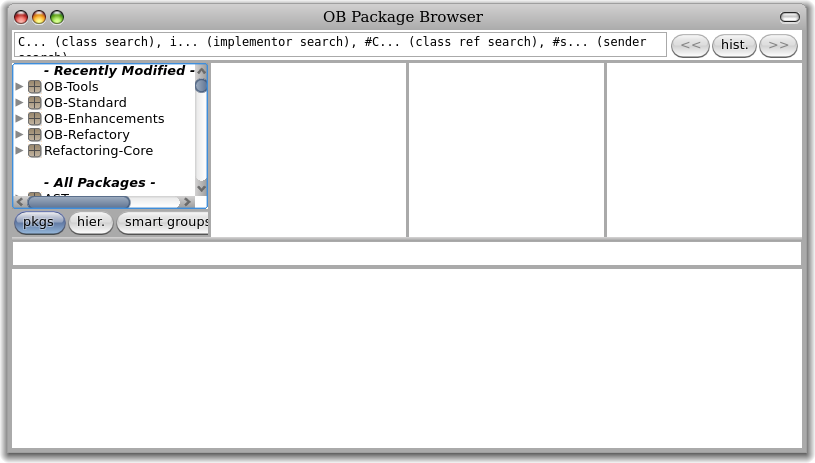
\includegraphics[width=\textwidth]{SystemBrowser0} }
	 {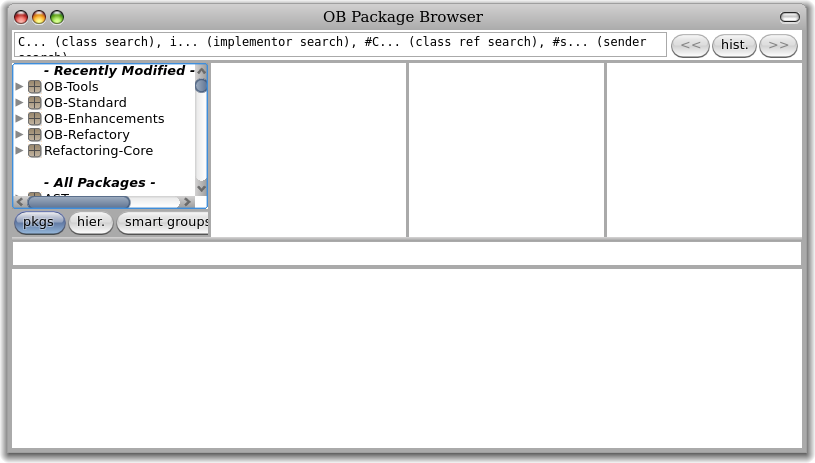
\includegraphics[width=0.7\textwidth]{SystemBrowser0} }
   \caption{Browser}
   \figlabel{SystemBrowser0}
\end{figure}

Browser上部の4つの小さなペインはシステム内メソッドの階層ビューを表しています。これはディスク上のファイルを見るためのNeXTstepの\textit{File Viewer}やMac OS Xの\textit{Finder}のカラムモードと同様のビューを提供しています。左端のペインはクラスの\emph{パッケージ}リストです。その内の1つ(例えば\scat{Kernel})を選択するとすぐ右隣にあるペインにパッケージ中のすべてのクラスが表示されます。
% \on{I adopted the spelling of NeXTstep recommended by wikipedia}

\begin{figure}[htbp]
   \centering
   \ifluluelse
	   {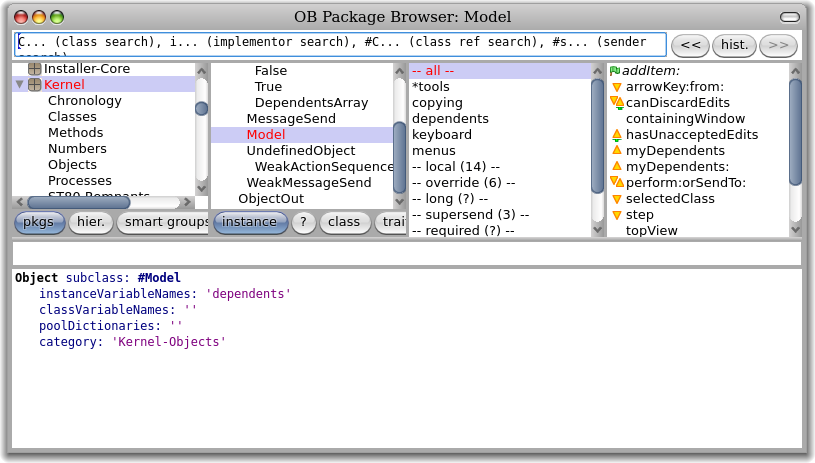
\includegraphics[width=\textwidth]{SystemBrowser1} }
	   {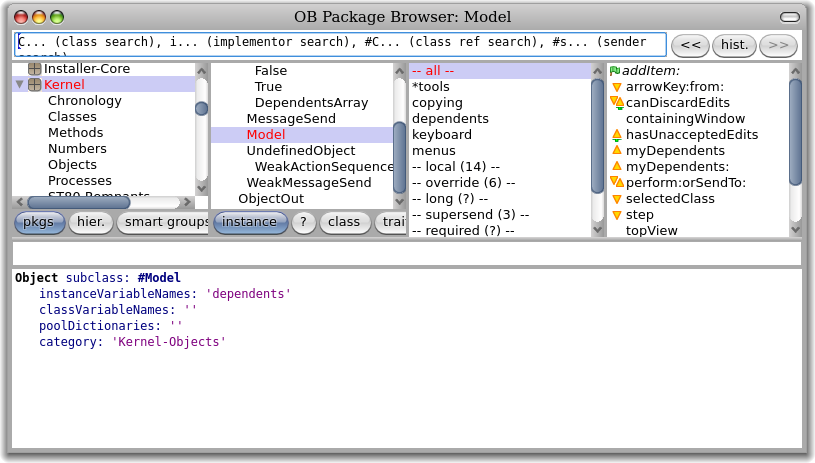
\includegraphics[width=.7\textwidth]{SystemBrowser1} }
   \caption{Browserで\ct{Model}クラスを選択
   \figlabel{SystemBrowserModel}}
\end{figure}

同様に左から2番目のペインでクラスの中の1つ、例えば\menu{Model}(\figref{SystemBrowserModel}参照)を選択すると左から3番目のペインに、そのクラスに対して定義された\emph{プロトコル}が表示されます。すると仮想プロトコル\prot{-{}-all-{}-}がデフォルトで選択されます。プロトコルはメソッドをカテゴリー化するためのもので、概念的に首尾一貫して細分化することにより、クラスを見つけたりその振る舞いを考えたりするのを助けてくれます。
左から4つめのペイン選択したプロトコルで定義された全てのメソッド名が表示されます。メソッド名を選択すると、そのメソッドのソースコードがBrowser下部にある大きなペインに表示されます。そのペインではソースコードを閲覧したり、編集したり、編集後のソースコードを保存したりすることができます。\menu{Model}クラスから,\protind{dependents}プロトコル、そして\menu{myDependents}へと選択すると、\figref{SystemBrowserMyDependents}のように表示されるはずです。
\protindex{all}
\cmindex{Model}{myDependents}

\begin{figure}[htbp]
   \centering
   \ifluluelse
	   {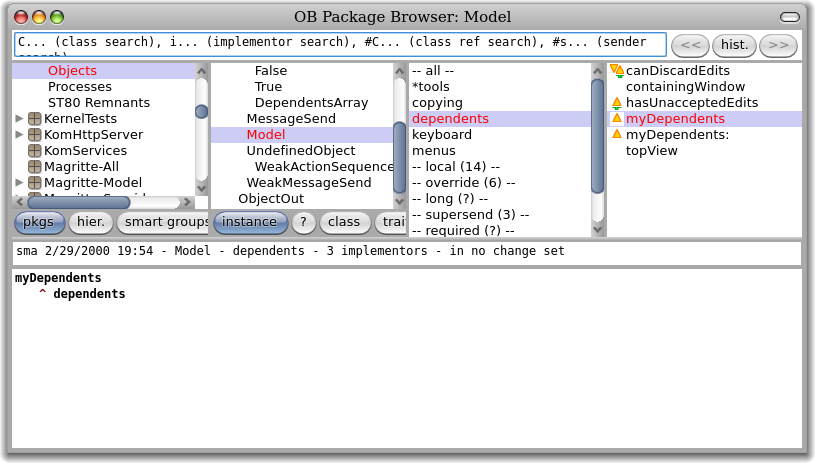
\includegraphics[width=\textwidth]{SystemBrowserMyDependents}}
	   {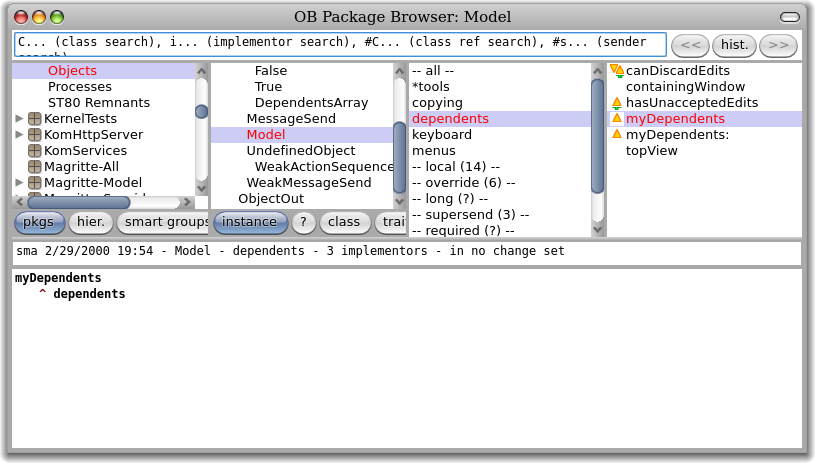
\includegraphics[width=0.7\textwidth]{SystemBrowserMyDependents}}
   \caption{\ct{Model}クラスの\ct{myDependents}メソッドをBrowserで表示
   \figlabel{SystemBrowserMyDependents}}
\end{figure}

Mac OS X の\emph{Finder}とは違い、Browser上部4つのペインはディレクトリではありません。
クラスやメソッドは\st 言語の一部であるのに対し、パッケージとプロトコルはそうではありません。パッケージとプロトコルはそれぞれのペインに表示する必要がある情報量を制限するのに役立てるために導入されたものです。たとえば、もしプロトコルがなければ、選択したクラスの全てのメソッドのリストをBrowserに表示するでしょう。多くのクラスでは、このリストは大きすぎて効率良く操作できません。 
\index{Mac OS X Finder}

このことにより、新パッケージや新プロトコルを作る方法は、新クラスや新メソッドを作る方法と異なっています。新パッケージを作るためにはパッケージペインで\actclick し\menu{new package}を選択します。新プロトコルを作るためにはプロトコルペインで\actclick し\menu{new protocol}を選択します。
ダイアログの中に新パッケージや新プロトコルの名前を入力すれば完了です。その作業後はパッケージやプロトコルの名前とその内容以外何も表示されないはずです。
\index{package!creating}

\begin{figure}[htbp]
   \centering
   \ifluluelse
	   {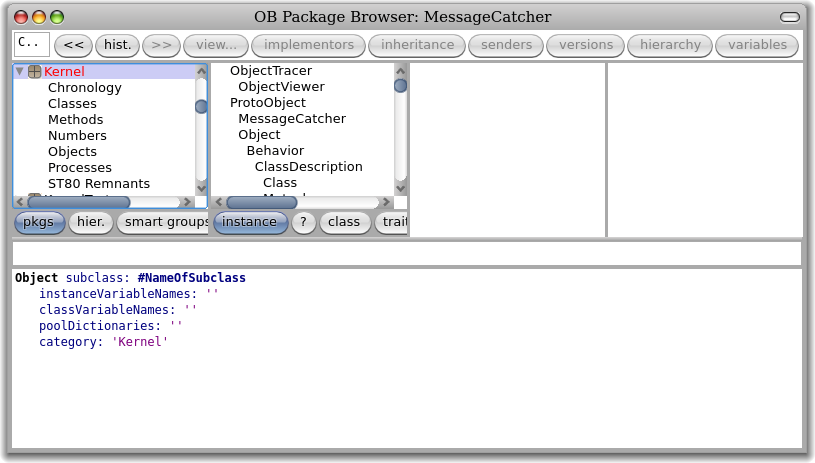
\includegraphics[width=\textwidth]{SystemBrowserClassCreation}}
	   {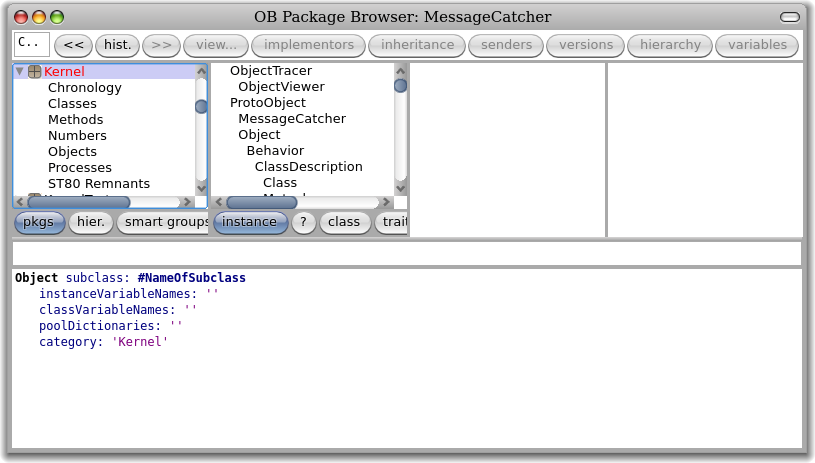
\includegraphics[width=0.7\textwidth]{SystemBrowserClassCreation}}
   \caption{クラス作成テンプレートをBrowserに表示
   \figlabel{SystemBrowserClassCreation}}
\end{figure}

新クラスや新メソッドを作るのとは対照的に、新パッケージや新プロトコルを作成するときには何らかの\st のコードを書かなくてはいけません。(左端のぺいんにある)現在選択されているパッケージをクリックするとBrowserペインのボタンが、クラス作成テンプレートを表示します(\figref{SystemBrowserClassCreation})。テンプレートを編集し新クラスを作ります。\ct{Object}の箇所を、今すでにありサブクラスを作りたいと思うクラスに置き換えて下さい。\ct{NameOfSubclass}の箇所を、新サブクラスに置き換えて下さい。もし既に決めているのであればインスタンス変数名を入れてください。新クラスのためのカテゴリーは、デフォルトでは現在選択しているパッケージのカテゴリーとなります\footnote{パッケージとカテゴリーが正確には同じものではないことを思い出して下さい。\secref{packages}にてそれらの関係について詳しく見ていきます}。しかしこれはもし望むのであれば変更することはできます。もし作りたいサブクラスの元となる既存のクラスを既にBrowserで見ているのならば、クラスペインを\actclick し\menu{class templates \ldots \go subclass template}を選択することにより、少しだけ初期化処理が違いますが、同じテンプレートを得ることができます。また既存のクラス定義を編集し、クラス名を何か新しいものに変更することでも、テンプレートの替りにすることができます。全てのケースにおいて、新しい定義をacceptしたときに、(\ct{#}から始まる名前の)新クラスが(対応するメタクラスとして)作られます。クラスを作ることは、そのクラスを参照するグローバル変数を作ることでもあります。それは全ての既存のクラスをそれらの名前を参照することができる理由です。
\index{class!creation}
\index{browser!defining a class}

新クラス名が(\ie \ct{#}で始まる)\lclsind{シンボル}としてクラスの作ったテンプレートの中に現れる理由や、クラスが作られた後、(\ie \ct{#}のない)識別子としてクラス名を使うことでそのクラスをコードから参照することができます理由が理解できたでしょうか?

新メソッドを作るプロセスも同様です。最初にメソッドを作りたいクラスを選択します、その後プロトコルを選択します。\figref{SystemBrowserMethodTemplate}にあるように、Browserは編集することのできるメソッド作成テンプレートを表示します。
\index{method!creation}
\index{browser!defining a method}

\begin{figure}[htbp]
   \centering
   \ifluluelse
	   {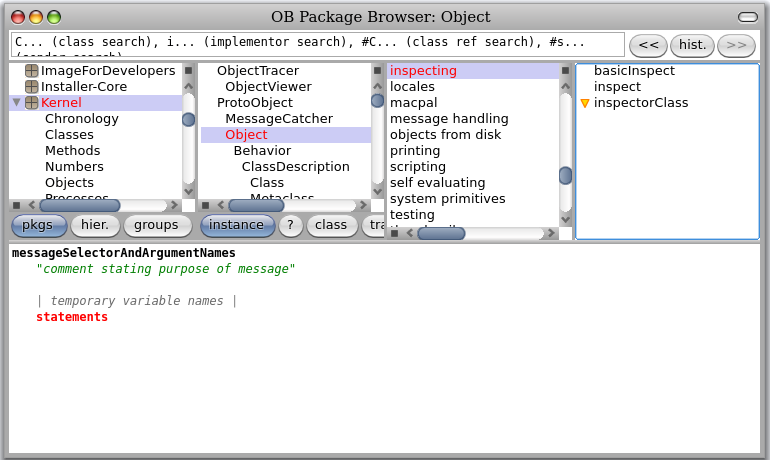
\includegraphics [width=\textwidth]{SystemBrowserMethodTemplate}}
	   {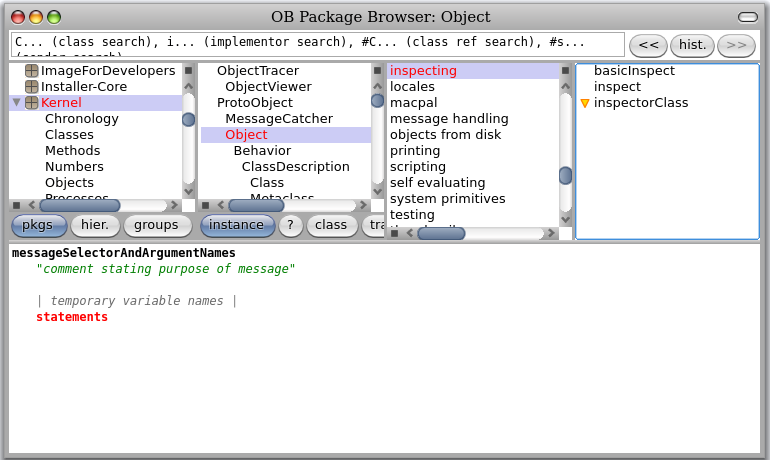
\includegraphics[width=0.7\textwidth]{SystemBrowserMethodTemplate}}
   \caption{メソッド作成テンプレートをBrowserに表示
   \figlabel{SystemBrowserMethodTemplate}}
\end{figure}

%---------------------------------------------------------
\subsection{コード空間を渡り歩く}

Browserはコードを探したり分析するためのいくつかのツールを提供します。様々なコンテキストメニューを\actclick することにより、もしくは最も頻繁に使われるツールの場合はキーボードショートカットにより、これらのツールを使うことができます。

\subsubsection{新しいBrowserウインドウを開く}
\seclabel{browsing}

いくつかのBrowserウインドウを開きたいと思うときがあると思います。コードを書いているときは少なくとも2つ: 1つは打ち込んでいるメソッドのため、もう1つはシステム周りがどのように動いているのかを見るためです。クラス名上で何かテキストを選択し\ind{キーボードショートカット}\short{b}を使うことでBrowserを開くことができます。
\index{browser!browse button}
\index{keyboard shortcut!browse it}

\dothis{次のことを試してみてください: workspaceウインドウ内でクラス名(たとえば\ct{Morph})を打ち込み、それを選択し\short{b}を押して下さい。この方法はよく役に立ち、どのテキストウィンドウでも使えます。}

\subsubsection{センダーとメッセージ作成者}
\seclabel{sendersImplementors}

\index{browser!senders}
メソッドペインで\menu{browse \ldots \go senders (n)}を\actclick すると、選択したメソッドを使用している全てのメソッドのリストが表示されます。Browserを開き\ct{Morph}を選択し、メソッドペインの中の\mthind{Morph}{drawOn:}メソッドをクリックすると、\ct{drawOn:}本体がBrowser下部に表示されます。 \menu{senders (n)} (\figref{SendersOfDrawOn})を選択すると、\ct{drawOn:}を一番上の項目として下に向かって\ct{drawOn:}が送る全てのメッセージ(\figref{SendersOfDrawOn2})のメニューが表示されます。 このメニューの中の項目を選択すると、選択したメッセージ(\figref{CanvasDraw})を送る、イメージファイル内の全メソッドのリストをbrwoserで開きます。

%\begin{figure}[htb]
%\begin{minipage}[b]{0.74\textwidth}
%\centerline {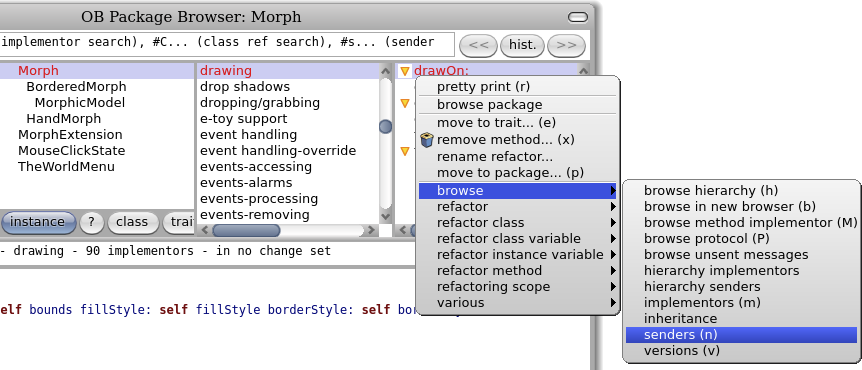
\includegraphics[width=\textwidth]{SendersOfDrawOn}}
%\caption{The \menu{senders (n)} menu item.\figlabel{SendersOfDrawOn}}
%\end{minipage}
%\hfill
%\begin{minipage}[b]{0.24\textwidth}
%\centerline {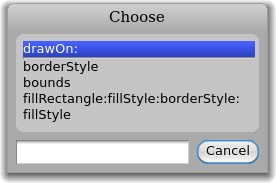
\includegraphics[width=\textwidth]{SendersOfDrawOn2}}
%\caption{Choose senders of which message.\figlabel{SendersOfDrawOn2}}
%\end{minipage}
%\end{figure}

\begin{figure}[htb]
\centerline {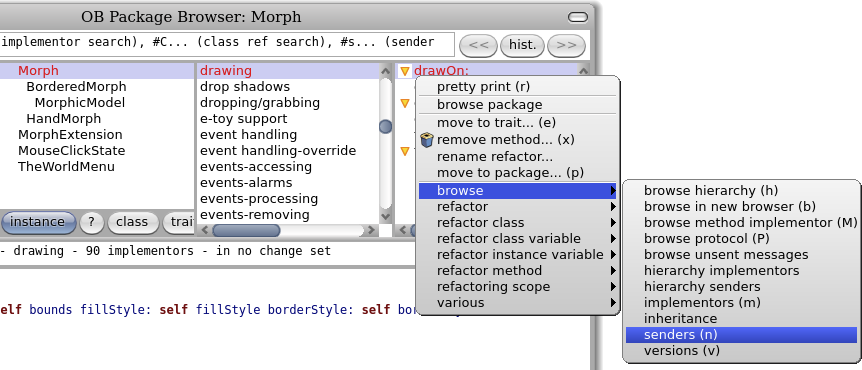
\includegraphics[width=\textwidth]{SendersOfDrawOn}}
\caption{\menu{senders (n)}メニュー項目。\figlabel{SendersOfDrawOn}}
\end{figure}

\begin{figure}[htb]
\centerline {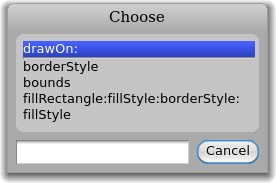
\includegraphics[width=0.4\textwidth]{SendersOfDrawOn2}}
\caption{メッセージのセンダーを選択。\figlabel{SendersOfDrawOn2}}
\end{figure}

\menu{senders (n)}の中の``n''はキーボードショートカットがあることを伝えています。メッセージのセンダーを探すためのキーボードショートカットは\short{n}となります。この方法は、\emph{どの}テキストウインドウでも使えます。

\dothis{コードペインにある``drawOn:''テキストを選択し、\short{n}を押すと、すぐに\ct{drawOn:}のセンダーが表示されます。}

\begin{figure}[htbp]
	\begin{center}
   \ifluluelse
		{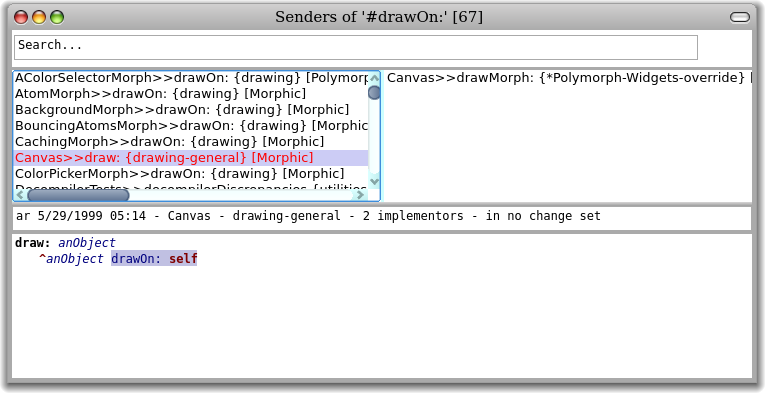
\includegraphics[width=\textwidth]{CanvasDraw}}
		{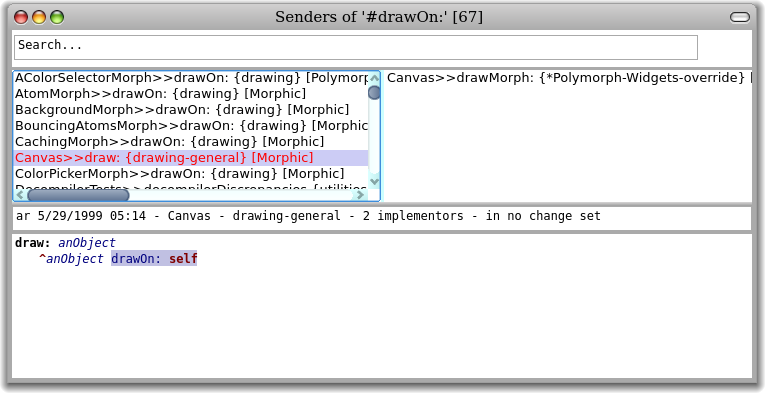
\includegraphics[width=0.7\textwidth]{CanvasDraw}}
	\end{center}
	\caption{Senders Browserは \ct{Canvas>>>draw}メソッドが\ct{drawOn:}メッセージをその引数としていることを表しています。\figlabel{CanvasDraw}}
\end{figure}

\ct{AtomMorph>>>drawOn:}にある\ct{drawOn:}センダーを探すとき、これはスーパークラスが\subind{super}{送信}していることがわかるでしょう。そのためこのメソッドは\ct{AtomMorph}のスーパークラスが実行していることがわかります。これは何のクラスなんでしょう? ~ \menu{browse \go hierarchy implementors}を\actclick するとそれが\ct{EllipseMorph}クラスであることがわかります。 
\index{browser!hierarchy button}

\figref{CanvasDraw}に示されている、リストにある6番目のセンダー、\ct{Canvas>>>draw}、を見てみましょう。このメソッドは\ct{drawOn:}を、それが引数として受け渡される全てのオブジェクトや、任意のクラスのインスタンスとなる可能性があるオブジェクトに対し、送信していることがわかります。
データフロー解析はいくつかのメッセージのレシーバークラスを理解する助けになります。しかし一般的に、Browserを使い、どのメッセージ送信がどのメソッドの実行につながるのかを知る簡単な方法はありません。このような理由から``senders'' Browserは、選択したセレクターと一緒にメッセージの全センダー名を連想させるものを正確に示します。
senders Browserはそれだけでなく、どのようにメソッドを\emph{使う}のかを理解する必要があるときに、即座にそのメソッドの使用例へ導いたりするなど、非常に役立ちます。
同じセレクターによる全てのメソッドは同じように使われるべきであるため、定められたメッセージの使い方は似ています。
\index{browser!senders}

\index{browser!implementors}
implementors Browserも似たような動作をします。しかしメッセージのセンダーリストの替りに、同じセレクターを使ったメソッドによって実装した全クラスのリストを表示します。これを見るためにはメソッドペインにある\lct{drawOn:}を選択し、そして\menu{browse \go implementors (m)}を選択して下さい(もしくはコードペインにある``drawOn:''テキストを選択し、\short{m}を押して下さい)。そうすればメソッドのリストウインドウが表示され、スクロールすると90余りのクラスが\ct{drawOn:}メソッドを実装していることがわかります。非常に多くのクラスがこのメソッドを実装しているということだけが驚くことではありません。\ct{drawOn:}は、それ自身をスクリーン上に描写することができる全てのオブジェクトによって理解されるメッセージなのです。
\subsubsection{メソッドのバージョン}
\seclabel{versions}

メソッドの新しい\subind{method}{version}を保存すると、古いものは失われます。\pharo は全ての古いバージョンを保存し、異なるバージョンを比較したり、古いバージョンに戻したり(``復帰'')することができます。
\begin{figure}[btp]
   \centering
   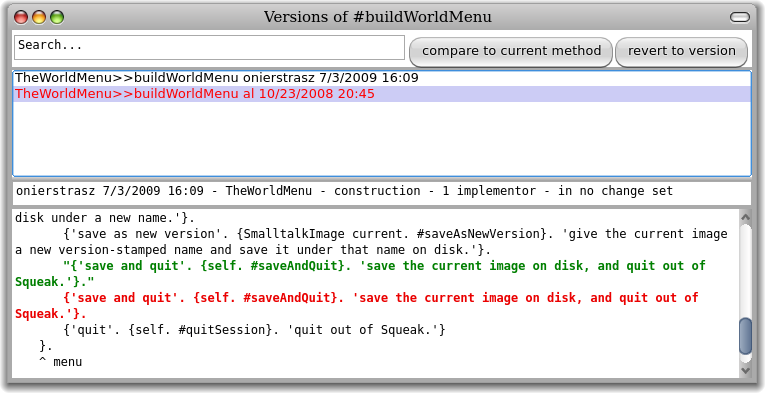
\includegraphics[width=\textwidth]{Versions}
   \caption{\ind{Versions Browser}が2つの\ct{TheWorldMenu>>>buildWorldMenu:}メソッドを表示}
   \figlabel{buildWorldMenuVersions}
\end{figure}
\menu{browse \go versions (v)}メニューアイテムにより、選択したメソッドの連続して修正することができます。\figref{buildWorldMenuVersions}では\ct{buildWorldMenu:}メソッドの2つのバージョンを示しています。

\index{browser!versions button}
表示されている上部のペインには、そのメソッドのそれぞれのバージョンの1行が表示されています。そこではこのメソッドを書いたプログラマーのイニシャル、保存した日付、クラス名とメソッド名、そしてそれらが定義されているプロトコルを尋ねてきます。
現在の(アクティブな)バージョンはリストの一番上にあります。どちらのバージョンが選択されてもそれは下のペインに表示されます。
% If the \menu{diffs} checkbox is selected, as it is in \figref{mouseUpVersions}, the display also shows the differences between the selected version and the one immediately older. 
選択されたメソッドと現在のバージョンの違いを表示したり、選択したバージョンを復帰するためのボタンも用意されています。
% The \menu{prettyDiffs} checkbox is useful if there have been changes to layout: it pretty-prints both versions before differencing, so that the differences that are displayed exclude formatting changes. 

\ind{Versions Browser}があるのはコードを提供するときに、もはや必要ないので削除したほうが良いかどうかを悩まなくても済むようにするためにあります。
もしそのコードが\emph{本当に}必要だと分かったら、いつでも古いバージョンに復帰することができます。また古いバージョンから必要なコードの断片を得、別のメソッドに貼り付けることもできます。
今使っているバージョンで、もはや必要のないコードをコメントアウトするのは悪い習慣です。なぜならそれによって現在のコードが読みにくくなるからです。Smalltalkerは読みやすいコードを非常に高く評価します。

\hint{もしメソッド全体を削除した後、それを戻そうと決めた場合はどうすればいいでしょう? change setの中に削除したものを見つけることができます。そこで\actclick することにより以前のバージョンを見るかどうかを確認することができます。
Change Set Browserは\secref{env:changeSet}に表示されています。}

\subsubsection{メソッドのオーバーライド}
\seclabel{overriding}

inheritance Browserは、表示されたメソッドによって全てのオーバーライドされたメソッドを表示します。それらどのように動作するかを見るには、Browserにある\cmind{ImageMorph}{drawOn:}メソッドを選択してください。
(\figref{OBinheritanceBrowser})メソッドの隣にある三角形のアイコンに注目してください。
上向きの三角形は\ct{ImageMorph>>>drawOn:}が継承されたメソッドであること(\ie \ct{Morph>>>drawOn:})を教えてくれます。そして下向きの三角形はそれがサブクラスによってオーバーライドされたことを教えてくれます。(アイコンをクリックすることで、これらのメソッドを操作することもできます。)
では\menu{browse \go inheritance}を選択してください。
inheritance Browserによりオーバーライドされたメソッドの階層関係を見ることができます。(\figref{OBinheritanceBrowser}参照)

\begin{figure}[btp]
	\begin{center}
   \ifluluelse
		{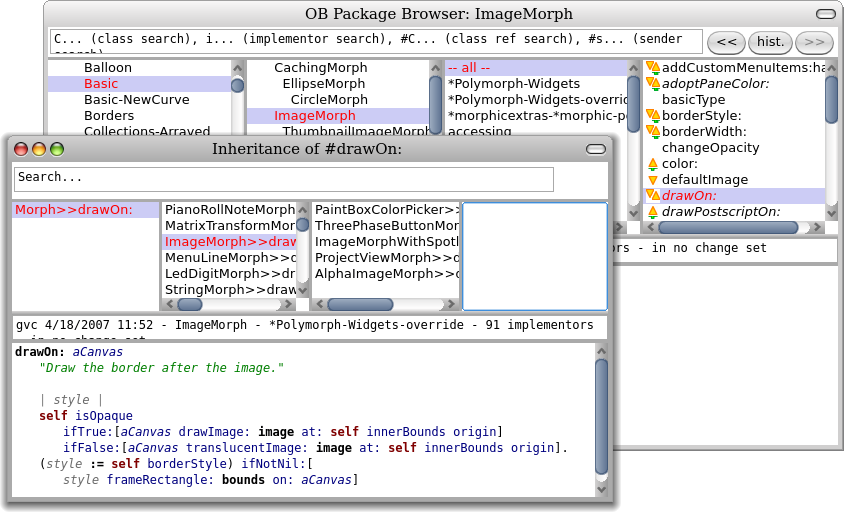
\includegraphics[width=\textwidth]{OBInheritanceOverriding}}
		{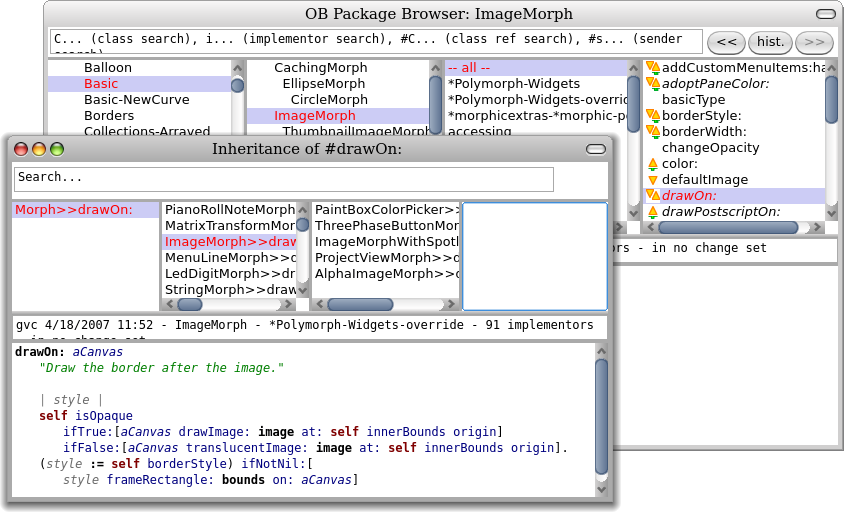
\includegraphics[width=0.7\textwidth]{OBInheritanceOverriding}}
	\end{center}
	\caption{\ct{ImageMorph>>>drawOn:} とそれがオーバーライドしたメソッド。選択したメソッドの兄弟関係がリストに表示されている。}
	\figlabel{OBinheritanceBrowser}
\end{figure}

\subsubsection{階層ビュー}
\seclabel{hierarchy}

標準では、Browserは左端のペインにパッケージのリストを表示します。
しかしクラスの階層ビューを入れ替えることは可能です。
関心のある特定のクラスを選択してください。例えば\ct{ImageMorph}を選択し、\button{hier.}ボタンをクリックしてください。
選択したクラスの全てのスーパークラスとサブクラスの階層関係が、左端のペインで見ることができます。
2つ目のペインは選択したクラスで実装されているメソッドのパッケージがリスト表示されています。
%The \button{hierarchy} button opens a \ind{hierarchy browser} on the current class; this
%browser can also be opened by using the \menu{browse hierarchy} menu item in the class pane.
%The hierarchy browser is similar to the browser, but instead of displaying the categories and the classes in each category, it shows a single list of classes, indented to represent inheritance.
%The category of the selected class is displayed in the small annotation pane at the top of the browser.
\figref{hierarchyBrowser}では、hierarchy Browserが\clsind{ImageMorph}のスーパクラスが \clsind{Morph}であることを示しています。
\index{browser!hierarchy button}

\begin{figure}[btp]
	\begin{center}
	\ifluluelse
		{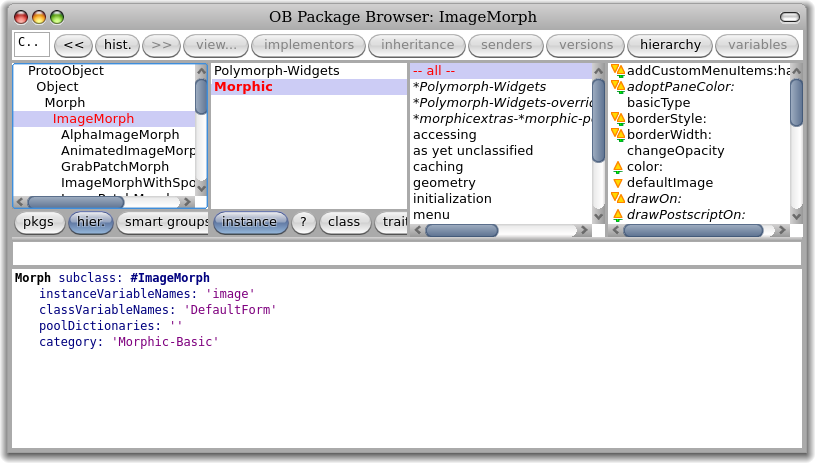
\includegraphics[width=\textwidth]{hierarchyBrowser}}
		{\includegraphics[width=0.7\textwidth]{hierarchyBrowser}}
	\end{center}
	\caption{\ct{ImageMorph}の階層ビュー。}
	\figlabel{hierarchyBrowser}
\end{figure}

\subsubsection{参照している変数を見つける}
\seclabel{variables}

\index{browser!variables}
クラスペインであるクラスを\actclick し、\menu{browse \go chase variables}を選択することで、インスタンス変数やクラス変数が使われている箇所を見つけることができます。

\emph{chasing Browser}を使うことで、全てのインスタンス変数とクラス変数、次にこれらのアクセサーを送るメソッド、そしてその他と順番にアクセサーを見ることができます(\figref{chasingBrowser})。

\begin{figure}[btp]
	\begin{center}
	\ifluluelse
		{\includegraphics[width=\textwidth]{chasingBrowser}}
		{\includegraphics[width=0.7\textwidth]{chasingBrowser}}
	\end{center}
	\caption{\ct{Morph}のためのchasing Browser。}
	\figlabel{chasingBrowser}
\end{figure}

% The menu also includes \menu{inst var defs}, which shows the subset of the instance variable references that assign to the variable. 
%Once you click on the button or select the menu item, you will be presented with a dialog that invites you to choose a variable from all of the variables defined in the current class, and all of the variables that it inherits.  The list is in inheritance order; it can often be useful to bring up this list just to remind yourself of the name of an instance variable.  If you click outside the list, it will go away and no variable browser will be created.

%Also available by \actclick{ing} the class pane is \menu{class vars}, which opens an inspector showing the class variables of the current class \emph{and their values}, and \menu{class refs (N)} which displays a list of all of the methods that directly reference the current class.

\subsubsection{ソース}
\seclabel{sources}

\index{browser!view}
メソッドペインを\actclick することで利用可能な\menu{various \go view \ldots}メニューアイテムにより、sourceペインで選択したメソッドをどのように見せるかを可能にする``how to show''メニューを表示します。\menu{source}のソースコード、\menu{prettyPrint}表示されたソースコード、そして\menu{byteCode}とバイトコードから\menu{decompile}されたソースコードといったオプションも選択できます。
% The label on the button changes if you select one of the other modes.  There are other options too; if you let the mouse linger over the names, a help balloon will appear.  Try some of them.
\index{method!pretty-print}
\index{method!decompile}
\index{method!byte code}

``how to show''メニューで選択した\menu{prettyPrint}はセーブする前に整形出力したメソッドと同じもの\footnote{\menu{pretty print (r)}はメソッドペインの最初のメニューアイテムもしくはcodeペインの真ん中下側にあります。}ではないことに注意してください。このメニューは、Browserがどのように表示するかを単に操作するだけで、システムに保存されたコードに対しては何の影響も与えません。2つのBrowserを開き、一方のBrowserで\menu{prettyPrint}を選択し、もう一方のBrowserで\menu{source}を選択することにより、このことを確認することができます。実際、2つのBrowserで同じメソッドを一方で\menu{byteCode}を選択し、もう一方で\menu{decompile}選択することで\pharo の仮想マシンのバイトコード化命令セットについて学ぶことができます。

\subsubsection{リファクタリング}

contextualメニューから多くの標準的なリファクタリングができます。4つのうちのどのペインを\actclick しても、現在リファクタリングすることが可能なものを見ることができます。\figref{refactoring}参照。

以前は、リファクタリングをするためにはrefactoring Browserと呼ばれる特殊なBrowserを使う必要がありましたが、現在はどのBrowserからもアクセスすることができます。

\begin{figure}[btp]
	\begin{center}
	\ifluluelse
		{\includegraphics[width=\textwidth]{refactoring}}
		{\includegraphics[width=0.7\textwidth]{refactoring}}
	\end{center}
	\caption{リファクタリング操作。}
	\figlabel{refactoring}
\end{figure}

%---------------------------------------------------------
\subsection{Browserのメニュー}

Browserペインを\actclick することで多くの追加機能を利用することができます。たとえメニューアイテム上のラベルが同じであっても、その\emph{意味}は文脈に依存します。例えばパッケージペイン、クラスペイン、プロトコルペイン、そしてメソッドペイン全てが\menu{File out}メニューアイテムを持っています。しかしそれらは違う動作をします。パッケージペインの\menu{File out}メニューはパッケージ全てをファイル出力します。クラスペインの\menu{File out}メニューは全てのクラスをファイル出力します。プロトコルペインの\menu{File out}メニューは全てのプロトコルをファイル出力します。そしてメソッドペインの\menu{File out}メニューは表示されたメソッドだけをファイル出力します。このことはすぐに分かることのように見えるかもしてませんが、初心者にとっては混乱の元になりえます。
\index{file!filing in}
\index{file!filing out}

おそらくパッケージペインの中で最も便利なメニューアイテムは\menu{find class\ldots (f)}です。カテゴリは活発に開発しているコードのために役立ちますが、システム全体のカテゴライズ化について、ほとんどの人は知りません。また、探しているクラスがどのパッケージにあるのか推測するために、クラス名の最初の数文字を打ち込んだ後に続けてshort{f}と打ち込んだ方がはるかに速いということもほとんどの人は知りません。\menu{recent classes\ldots}はたとえクラス名を忘れてしまったとしても、最近閲覧したクラスへ素早く戻るのに役立ちます。
\index{class!finding}
\index{class!recent}

特定のクラスやメソッドも、Browserの左上にある検索ボックスにその名前を打ち込むことで探すことができます。リターンキーを打ち込むと検索が始まりシステムを一時的に停止し、その後検索結果を表示します。検索語の前に\ct{#}を付けることで、クラスを参照しているものや、メッセージを送信したクラスをさがすことができることに注目してください。
%To browse to a particular method, you can 
%In the class pane, there are two menu items \menu{find method} and \menu{find method wildcard\ldots} that can be useful if you want to browse a particular method.  
もしあるクラスの特定のメソッドを探しているのなら、\prot{-{}-all-{}-}プロトコルで閲覧する方が速い時があります(これはデフォルトです)。メソッドペインにマウスを移動し、探しているメソッド名の最初の文字を打ち込んでください。この方法により探しているメソッド名が表示されるよう、ペインがスクロールします。
\index{method!finding}
\protindex{all}

\dothis{\cmind{OrderedCollection}{removeAt:}で2つの操作方法を試してください。}

その他多くのオプションがメニューにはあります。これを使うことでBrowser上の作業や何がどこにあるのか探すのに費やす時間を減らすことができます。
\dothis{クラスペインメニューの\menu{Browse Protocol}, \menu{Browse Hierarchy}, そして\menu{Show Hierarchy}を実行した結果を比較してください。}

%---------------------------------------------------------
\subsection{プログラムでBrowserを操作}

\glbind{SystemNavigation}クラスはシステム周りを操作するために役に立つユーティリティメソッドのいくつかを提供しています。その機能の大半は古典的なBrowserにより提供され、\ct{SystemNavigation}によって実装されます。\index{browsing programmatically}

\dothis{
workspaceを開き、\ct{drawOn:}:センダーを見るために以下のコードを評価してください。}
\begin{code}{}
SystemNavigation default browseAllCallsOn: #drawOn:
\end{code}
特定のクラスのメソッドへのセンダーを検索を制限するためには次のようにコードを評価してください。
\begin{code}{}
SystemNavigation default browseAllCallsOn: #drawOn: from: ImageMorph
\end{code}
開発ツールもオブジェクトなので、プログラムからそれらに完全にアクセスすることができます。そのため独自のツールを開発したり、今あるツールを必要に応じて取り込むこともできます。

\menu{implementors}メニューアイテムと同じ動作をプログラム上行うには次のように評価してください。
\begin{code}{}
SystemNavigation default browseAllImplementorsOf: #drawOn:
\end{code}

他に何が出来るのかを知るにはBrowserで\ct{SystemNavigation}クラスを探してみてください。もっと多くの操作例についてはFAQ(\appref{faq})で見つけることができます。

%=========================================================
\section{Monticello}

\secref{Monticello}において、\pharo のパッケージ作成ツール、\ind{Monticello}の概要についてお見せしました。しかしMonticelloは、その章に書かれていた以上の機能を持っています。Monticelloは\emph{パッケージ}を扱うため、Monticelloについてお伝えする前に、\ind{パッケージ}とは何なのかについて正確に説明する必要があります。

%---------------------------------------------------------
\subsection{\pharo コードを宣言型のカテゴリー化}\seclabel{packages}

\secref{categoriesPackages}において、パッケージとは多かれ少なかれカテゴリーと同等のものであると指摘しました。これからそれらの関係について詳しく見ていきましょう。
パッケージシステムは、カテゴリーとプロトコルのために開発された単純な命名規則を活用した\st ソースコードを簡単で軽量にまとめる方法の1つです。

例を使って説明しましょう。\pharo からリレーショナル型データベースを簡単に使うために命名されたフレームワークを開発していると思ってください。このフレームワークを\ct{PharoLink}と呼ぶことにします。そして作った全てのクラスを含む一連のカテゴリーを作ったとします。
例えば、\ct{'PharoLink-Connections'}カテゴリーは\ct{OracleConnection MySQLConnection PostgresConnection}を含み、 \ct{'PharoLink-Model'}カテゴリーは\ct{DBTable DBRow DBQuery}等を含みます。ただし、これらのクラスの中に作ったコード全てが含まれていないこととします。例えばSQLが扱いやすい形式にオブジェクトを変換する一連のメソッドがあるかも知れません。

\begin{code}{}
Object>>>asSQL
String>>>asSQL
Date>>>asSQL
\end{code}

\noindent
% \damien{don't we say 'belong to'?}
% \on{no -- belong in = they should be there; belong to = they are there}
これらのメソッドは、\ct{PharoLink-Connections}や\ct{PharoLink-Model}カテゴリとして同じパッケージに入っています。
しかし明らかに\ct{Object}クラス全体はパッケージの中に入っていません。そのため、クラスの残りの部分は別のパッケージに入れるとしても、特定の\emph{メソッド}を任意のパッケージに入れる方法が必要になります。
\index{package!extension}
\seeindex{extension package}{package, extension}

これらのメソッドを、prot{*PharoLink}(最初のアスタリスクに注意してください)と呼ばれる(\ct{Object}, \ct{String} \ct{Date}等)のプロトコルに置くことで、それは実現できます。\scat{PharoLink-\ldots}カテゴリーと\prot{*PharoLink}プロトコルの組み合わせにより\ct{PharoLink}と呼ばれるパッケージは形作られます。
正確に言うと以下のようにパッケージに納められるルールの事です。

\ct{Foo}と名付けられたパッケージは次のものを含みます。

\begin{enumerate}		\seclabel{packageRules}
	\item{} \scat{Foo}カテゴリ内もしくは\scat{Foo-}で始まる名前のカテゴリ内にある、クラスの全ての\emph{クラス定義}
	\item{} \label{env:extensions} \prot{*Foo}や\prot{*foo}\footnote{この比較を行うときには、名前の中にある大文字小文字は無視されます。}という名のプロトコル内もしくは\prot{*Foo-}や\prot{*foo-}で始まる名前のプロトコル内にある、\emph{任意のクラス}内の全ての\emph{メソッド}
	\item{} \scat{Foo}カテゴリー内もしくは\scat{Foo-}で始まる名前のカテゴリー内にある、クラス内の全ての\emph{メソッド}。ただし\prot{*}で始まる名前のプロトコル内にあるメソッドは\emph{除く}。
	
\end{enumerate}
\noindent
これらのルールの結果、各クラスの定義と各メソッドは、厳密に1つのパッケージに属するということになります。
最後のルールにある\emph{例外}があることを除き、これらのメソッドは他のパッケージに属している必要があります。ルール\ref{env:extensions}において無視するケースの理由は、慣習的にプロトコル名が通常は(必ずというわけではないですが)小文字(空白ふくまない)であることです。その一方でカテゴリー名はCamelCase(空白を含まない)を使います。
\index{camelCase}

\ct{PackageInfo}クラスはこれらのルールに従い実装されています。その結果の感触はこのクラスを試すことで得られます。

\dothis{workspace上で以下の式を評価して下さい。}

\begin{code}{}
mc := PackageInfo named: 'Monticello'
\end{code}

このパッケージについて深く考える事ができるようになりました。例えばworkspaceペイン上で\ct{mc classes}を表示することにより、Monticelloパッケージを構成するクラスの長いリストが返ります。

\ct{mc coreMethods}により、これらのクラスにある全てのメソッドのための\ct{MethodReference}のリストが返されます。
\ct{mc extensionMethods}はおそらく最も興味深い検索語でしょう。つまり\ct{mc extensionMethods}は\lct{Monticello}クラスを除き、\ct{Monticello}パッケージに含まれる全てのメソッドを返します。

パッケージは比較的新しく\pharo に追加されたものです。しかしパッケージの命名規則は、すでに使われているものがベースとなっているため、\ct{PackageInfo}を使用し明らかに命名規則に則っていない古いコードをも分析することができます。

\dothis{\ct{(PackageInfo named: 'Collections') externalSubclasses}を使いを\lct{表示}してください。この式により\ct{Collection}パッケージに含まれ\emph{ない}、\ct{Collections}の全てのサブクラスのリストが返ります。}

%---------------------------------------------------------
\subsection{Monticelloの基礎}

\ind{Monticello}は、合衆国3番目の大統領であり「the Statute of Virginia for Religious Freedom」の著者であるThomas Jeffersonの山頂の家にちなんで名付けられました。この名前の意味はイタリア語で``小さな山''であり、イタリア語の``c''、chairの``ch''の音を使いと一般的にMonticelloと発音されます。


\begin{figure}[btp]
	\begin{center}
	\ifluluelse
		{\includegraphics[width=\textwidth]{freshMonticello}}
		{\includegraphics[width=0.7\textwidth]{freshMonticello}}
	\end{center}
	\caption{Monticello Browser.}
	\figlabel{freshMonticello}
\end{figure}

Monticello Browserを開くと、\figref{freshMonticello}に示されるように2つのペインと1列に並ぶボタンが表示されます。左側のペインには、今動かしているイメージファイル内にロードされた全てのパッケージがリスト表示されています。また、名前の後にあるカッコの中にパッケージを特定するバージョンが表示されます。

右側のペインにはMonticelloが知っているソースコードリポジトリ全体のリストが表示されている。通常はそのリストからコードを読み込みます。左側のペインにあるパッケージを選択すると、右側のペインには選択したパッケージのバージョンを含んだリポジトリだけを表示するようフィルタリングされます。
リポジトリの1つは\emph{package-cache}と呼ばれるディレクトリーで、実行されているイメージファイルのあるディレクトリーの下にあるディレクトリーです。もし遠隔地にあるリポジトリーからコードを読み込んだり、書き込んだりする場合、そのコピーはpackage-cacheにも保存されます。ネットワークが使えないときでパッケージにアクセスする必要がある場合、このpackage-cacheは役立ちます。また、Monticelloファイル(.mcz)をemailの添付などで直接渡された場合、そのファイルをpackage-cacheディレクトリに入れるのが一番手軽な方法です。
\index{package!cache}

リストに新たなリポジトリを追加するには、\button{+Repository}ボタンをクリックし、ポップアップメニューからリポジトリーの種類を選択してください。ではHTTPリポジトリーを追加してみましょう。

\dothis{Monticelloを開き、\button{+Repository}ボタンをクリック。読むためのダイアログを編集します。}
%\ab{How does one continue the $\backslash$dothis to include the code?}
%\on{Don't.  Just close the \dothis{} and follow with the code.}
\needlines{4}
\begin{code}{}
MCHttpRepository
	location: 'http://squeaksource.com/PharoByExample'
	user: ''
	password: ''
\end{code}

\begin{figure}[btp]
	\begin{center}
	\ifluluelse
		{\includegraphics[width=0.7\textwidth]{SqueakSource-PBE}}
		{\includegraphics[width=0.7\textwidth]{SqueakSource-PBE}}
	\end{center}
	\caption{Repository Browser.}
	\figlabel{SqueakSource:PBE}
\end{figure}
\noindent
その後このリポジトリをRepository Browserを上に表示するため\button{Open}ボタンをクリックします。すると\figref{SqueakSource:PBE}のように見えるはずです。左側のペインはリポジトリー内の全てのパッケージのリストです。その内の1つを選択すると右側のペインにこのリポジトリー内にある選択されたパッケージの全てのバージョンが表示されます。

その内の1つのバージョンを選択すると、\button{Browse}ボタンを押すことで(イメージファイルに読み込むことなしに)閲覧でき、\button{Load}ボタンで読み込むことができ、\button{Changes}ボタンで選択したバージョンを読み込んだことによるイメージファイルの変更点を見ることができます。 また、\button{Copy}ボタンを押すことにより任意のバージョンのパッケージをコピーすることができ、そしてそれを別のリポジトリーに書きこむこともできます。

ご覧のように、バージョンの名前には、パッケージの名前、バージョンの作成者のイニシャル、およびバージョン番号が含まれています。バージョン名は、リポジトリー内のファイル名でもあります。これらの名前を変更してはいけません、なぜならMonticelloの動作とこれらの名前は依存関係にあるからです! Monticelloのバージョンファイルは単なるzipアーカイブであり、興味があればzipツール使用してファイルを解凍できます。しかしその内容を見る一番の方法は、Monticelloを使用することです。Monticelloでパッケージを作成するには、2つのことを行う必要があります。1つはいくつかのコードを書くこと、もう1つはそれについての情報をMonticelloに伝えることです。

\dothis{\scat{PBE-Monticello}と呼ばれるパッケージを作成し、\figref{MCnewcategory}に示すように2つのクラスをその中に置いて下さい。もちろん、\ct{Object}などの実在するクラスのメソッドを作成し、\pageref{sec:packageRules}ページにあるルールを用いて独自のクラスとして同じパッケージ内に置いて下さい\,---\,\figref{MCnewmethod}参照。}

\begin{figure}[btp]
	\begin{center}
	\ifluluelse
		{\includegraphics[width=\textwidth]{MCnewcategory}}
		{\includegraphics[width=0.7\textwidth]{MCnewcategory}}
	\end{center}
	\caption{``PBE''パッケージ中の2つのクラス。}
	\figlabel{MCnewcategory}
\end{figure}

\begin{figure}[btp]
	\begin{center}
	\ifluluelse
		{\includegraphics[width=\textwidth]{MCnewmethod}}
		{\includegraphics[width=0.7\textwidth]{MCnewmethod}}
	\end{center}
	\caption{``PBE''パッケージにこれから作成される拡張メソッド。}
	\figlabel{MCnewmethod}
\end{figure}

作ったパッケージをMonticelloに伝えるために、\button{+Package}ボタンをクリックして下さい。そしてパッケージ名、この場合は``PBE''を打ち込んで下さい。Monticelloは\ct{PBE}をパッケージリストに加えます。パケージの見出しがアスタリスクでマークされ、イメージ内のバージョンがまだどのリポジトリーにも書き込まれていないことを示しています。Monticelloに2つのパッケージがあることに注目して下さい。1つは\ct{PBE}、もう1つは\ct{PBE-Monticello}と呼ばれています。\ct{PBE}は\ct{PBE-Monticello}や\ct{PBE-}で始まる他の全てのパッケージを含みます。

最初はこのパッケージに関連している唯一のリポジトリーは\figref{MC+PBE}に示されているようにpackage-cacheだけです。それで問題はないので、コードをセーブして、package-cacheに書きこんで下さい。\button{Save}ボタンをクリックすると、\figref{PBE-on}のように、セーブするパッケージのバージョンのためのログメッセージを入力するよう求められます。このメッセージをAcceptするとMonticelloはパッケージをセーブします。セーブしたことを示すため、Monticelloのパッケージペインにマークされていたアスタリスクがなくなり、バージョン番号が付与されます。

もしパッケージに変更を加える\,---\,例えばクラスの1つにメソッドを追加する\,---\,場合、変更がセーブされていないことを示すため、アスタリスクが再度表示されます。package-cache上のRepository Browserを開くと、セーブしたバージョンを選択することや、\button{Changes}ボタンや他のボタンを押すことができます。リポジトリーに新たなバージョンを保存することもできます。\button{Refresh}ボタンを押し、リポジトリービューを一度更新して下さい。すると\figref{package-cache-browser}のようになるはずです。
\index{package!cache}

\begin{figure}[tbp]
	\begin{center}
		\includegraphics[width=\textwidth]{MC+PBE}
	\end{center}
	\caption{Monticello上ではPBEパッケージはまだ保存されていない。}
	\figlabel{MC+PBE}
\end{figure}

\begin{figure}[tbp]
	\begin{center}
	\includegraphics[width=0.8\textwidth]{PBE-on}
	\end{center}
	\caption{パッケージの新バージョンについてのログメッセージを入力する。}
	\figlabel{PBE-on}
\end{figure}

\begin{figure}[tbp]
	\begin{center}
	\includegraphics[width=\textwidth]{package-cache-browser}
	\end{center}
	\caption{package-cacheに今2つのバージョンのパッケージがあります。}
	\figlabel{package-cache-browser}
\end{figure}

新たなパッケージをpackage-cache以外のリポジトリーにセーブするためには、まず最初に、必要に応じてリポジトリーを追加するなどして、Monticelloにそのリポジトリーについて知らせる必要があります。その後package-cache Repository Browser内の\button{Copy}ボタンを使いコピーして下さい。\figref{associateRepository}に示されているように、リポジトリー上で\actclick し、メニューで\menu{add to package \ldots}を選択することで、特定のパッケージとお望みのリポジトリーを関連付けることができます。1度パッケージとリポジトリーを関連付けると、Monticello Browser内のリポジトリーやパッケージを選択し\button{Save}ボタンをクリックすることにより、新しいバージョンをセーブすることができます。もちろん書き込むリポジトリーへのパーミッションは必要です。
\emphind{\sqsrc}上の\ct{PharoByExample}リポジトリーは世界中いたる所で読むことができますが、書き込むことはできません。そのためそのリポジトリーにセーブしようとしてもエラーメッセージが表示されます。
ただし、\url{http://www.squeaksource.com}にあるWebのインターフェースから\sqsrc 上に独自のリポジトリーを作り、プログラムをセーブする場所として使うことはできます。
これは、作ったコードを友人と共有するためのメカニズムとして、特に役立ちます。

\begin{figure}[tbp]
	\begin{center}
		\includegraphics[width=\textwidth]{MCaddToPackage}
	\end{center}
	\caption{パッケージに関連付けられているリポジトリーのセットをリポジトリーに追加。}
	\figlabel{associateRepository}
\end{figure}

もしパーミッションのないリポジトリーに対しセーブをしようとすると、そのバージョンは意に反しpackage-cacheに書き込まれます。

それは、リポジトリの情報を編集したり(Monticello Browserで\actclick )、別のリポジトリを選択し、package-cache browserから\button{Copy}ボタンを押すことで復帰させることができます。

%=========================================================
\section{[Inspector]と[Explore]}
\seclabel{inspector} % (fold)

\st が他の多くの言語と異なる特徴の一つは、静的なコードの世界ではなく、生きたオブジェクトの世界への窓を提供していることです。
そこではどのようなオブジェクトでもプログラマーによって調べることが可能です。さらには変更することさえできます。\,---\, ただし、システムを構成している基本的なオブジェクトを変更するような時には注意が必要です。
もちろん言うまでもなく、まず最初にイメージを保存しておいてください!

%---------------------------------------------------------
\subsection{[Inspector]}

\dothis{\ind{[Inspector]}を使ってどんなことが出来るか、実際に見てみるために[Workspace]で \ct{TimeStamp now} と打ち込んで、\actclick したら \menu{inpect it}  を選択してください。}
(メニューを使う前にテキストを選択しておく必要はありません。もし、テキストを選択してない場合には、メニュー操作は現在の行全てを対象にするからです。 \menu{\textbf{i}nspect it} を選択する代わりに \short{i} とタイプしても同じです)

\clsindex{TimeStamp}
\index{keyboard shortcut!inspect it}

\begin{figure}[btp]
	\begin{center}
		\includegraphics[width=\textwidth]{inspectTimeNow1}
	\end{center}
	\caption{ \ct{TimeStamp now} をインスペクトする}
	\figlabel{inspectTimeNow1}
\end{figure}

\figref{inspectTimeNow1} のようなウィンドウが現れます。これが[Inspector]です。そしてこれはある特定のオブジェクトの内部に向かって開かれた窓と考えることができます。特定のオブジェクトとは、 \,---\, この場合には  \ct{TimeStamp now} という式を評価することによって生成された  \mbox{\ct{TimeStamp}} のインスタンスオブジェクトです。
ウィンドウのタイトルバーには、インスペクトしているオブジェクトの印字形式の表現が表示されています。左側のペインの先頭の \menu{self} を選択すると、右側のペインにそのオブジェクトが文字列で表示されます。
左側のペインはそのオブジェクトのツリー構造ビューとなっており、\self がツリーの根になっています。インスタンス変数は名前のそばにある三角形を展開することにより探索することができます。

[Inspector]の下部にある横長のペインは小さな[Workspace]のウインドウになってます。このウィンドウでは、偽変数の \ct{self} に左側のペインで選択したオブジェクトに束縛されているので便利です。そこで以下の式
\begin{code}{}
self - TimeStamp today
\end{code}
これをこの[Workspace機能のペイン]で \menu{inspect it} すると結果は \clsind{Duration} オブジェクトになります。
これは今日の夜中の0時と[Inspector]で見ている TimeStamp オブジェクトを生成した \ct{TimeStamp now} を評価した時点との間の時間を表しています。
さらに \ct{TimeStamp now - self} を評価するならば、あなたがこのセクションを読むのにどれくらい長い時間費やしたかを教えてくれます!

\ct{self} だけでなく、オブジェクトの全てのインスタンス変数は[Workspace機能のペイン]のスコープの範囲にあります。そのため式で参照することができるだけでなく代入することもできます。例えば、左のペインのツリーの根のオブジェクトを選択して、[Workspace機能のペイン]で \ct{jdn := jdn - 1} を評価すると、実際にインスタンス変数の \ct{jdn} が変化していることが分かりますし、さらに \ct{TimeStamp now - self} の値は1日分増えていることが分かります。

辞書オブジェクトや順序集合オブジェクトやコンパイルされたメソッドのオブジェクト、さらにいくつかのクラスに対しては、[Inspector]に特別な拡張がなされていて、これによりこれらのオブジェクトの内容をより簡単に検査することができます。

%---------------------------------------------------------
\subsection{[Object Explore]}

\emph{[Object Explore]}は概念的には[Inspector]とよく似ていますが、情報の表現の仕方が異なっています。この相違点を調べるためにさっきまでインスペクトしていたものと同じオブジェクトを\emph{[Explore]}で探検してみましょう。

\begin{figure}[tbp]
\begin{minipage}{0.48\textwidth}
	\begin{center}
	\ifluluelse
		{\includegraphics[width=\textwidth]{exploreTimeStampNow}}
		{\includegraphics[width=0.7\textwidth]{exploreTimeStampNow}}
	\end{center}
	\caption{ \ct{TimeStamp now} を探検する}
	\figlabel{exploreTimeStampNow}
\end{minipage}
\hfill
\begin{minipage}{0.48\textwidth}
	\begin{center}
	\ifluluelse
		{\includegraphics[width=\textwidth]{exploreTimeStampNow2}}
		{\includegraphics[width=0.7\textwidth]{exploreTimeStampNow2}}
	\end{center}
	\caption{インスタンス変数を探検する}
	\figlabel{exploreTimeStampNow2}
\end{minipage}
\end{figure}

\dothis{[Inspector]の左側のペインで \menu{self} を選択した状態で、\actclick して \menu{explore (I)} を選んでください}
\ind{[Explore]}のウインドウは \figref{exploreTimeStampNow} のような姿をしています。
\lct{ツリーの根} の次の小さな三角形をクリックすると、ビューは \figref{exploreTimeStampNow2} のように変化します。このビューは探検対象となっているオブジェクトのインスタンス変数を表示しています。
\ct{offset} のそばの三角形をクリックすると \emph{それが持つ}インスタンス変数が見えます。
\,---\,このように複雑な階層構造を探検しなければならない場合、[Explore]はその名の通りにたいへん便利です。
\index{keyboard shortcut!explore it}

[Explore]の[Workspace機能のペイン]の働きは[Inspector]のものとは若干異なります。
\ct{self} は必ずしもツリーの根のオブジェクトに束縛されておらず、現在選択しているオブジェクトを束縛するようになっており、選択されたオブジェクトのインスタンス変数も同様のスコープに従います。

[Explore]の真価を見るために、深い入れ子構造のオブジェクトを探検してみましょう。

\dothis{[Workspace]で \ct{Object explore} を評価してください}
これは \pharo の \ct{Object} クラスを表現するオブジェクトです。
メソッド辞書を表現するオブジェクトやこのクラスのコンパイルされたメソッドまでも直接ナビゲートすることが出来ることに注意してください( \figref{ExploreObject} 参照)。

\begin{figure}[tbp]
	\begin{center}
		\includegraphics[width=0.5\textwidth]{ExploreObject}
	\end{center}
	\caption{\ct{Object} クラスを探検する}
	\figlabel{ExploreObject}
\end{figure}

%\dothis{Open a browser, and \metaclick five times on the method pane to bring-up the Morphic halo on the \ct{OBPluggableListMorph} that is used to represent the list of messages. 
%Click on the \emph{debug} handle \debugHandle{} and select \menu{explore morph}
%from the menu that appears.  This will open an Explorer on the \clsind{OBPluggableListMorph} object that represents the method list on the screen.  
%Open the root object (by clicking in its triangle), open its \ct{submorphs}, and continue exploring the structure of the objects that underlie this Morph, as shown in \figref{explorePluggableListMorph}.}
%
%\begin{figure}[tbp]
%	\begin{center}
%		\includegraphics[width=0.7\textwidth]{explorePluggableListMorph}
%	\end{center}
%	\caption{Exploring a \ct{PluggableListMorph}}
%	\figlabel{explorePluggableListMorph}
%\end{figure}

%=========================================================
\section{[Debugger]}
\seclabel{debugger} % (fold)

\ind{[Debugger]} は間違いなく \pharo のツールの内もっとも強力なツールです。デバッグに利用されるだけでなく、新しいコードを書くのにも利用されます。
[Debugger]のデモンストレーションをするために、バグを作るところから始めましょう!

\dothis{ブラウザを使って以下のメソッドをクラス \ct{String} に追加してください}

\needlines{7}
\begin{method}[buggy]{バグがあるメソッド}
suffix
	"ファイル名と仮定して、最後のドットから後の部分をサフィックスとして返す"
	| dot dotPosition |
	dot := FileDirectory dot.
	dotPosition := (self size to: 1 by: -1) detect: [ :i | (self at: i) = dot ].
	^ self copyFrom: dotPosition to: self size 
\end{method}

こんな簡単なメソッドは動くのが当たり前だろうと確信して、SUnit のテストも書かずに、[Workspace]で \ct{'readme.txt' suffix} と打ち込んで \menu{print it(p)} を実行します。
すると驚いたことに、期待された答え \ct{'txt'} の代わりに、 \figref{PreDebugWindow} のような \clsind{PreDebugWindow} がポップアップしてきました。

\begin{figure}[btp]
	\begin{center}
	\includegraphics[width=0.8\textwidth]{PreDebugWindow}
	\end{center}
	\caption{ \ct{PreDebugWindow} によるバグの報告}
	\figlabel{PreDebugWindow}
\end{figure}

\ct{PreDebugWindow} はタイトルバーでどのようなエラーが起きたのか分かるようになっています。さらにエラーが起きるまでのメッセージの \emphind{スタックトレース} が表示されています。
トレースの一番下が始まりですが、 \ct{UndefinedObject>>DoIt} という行はコンパイルされて実行されたコードを表してます。それは、[Workspace]で \ct{'readme.txt' suffix} を選択して、\pharo に \menu{print it} を命令した時のものです。
もちろん、このコードは \clsind{ByteString} クラスのオブジェクト(\ct{'readme.txt'})にメッセージ \ct{suffix} を送信しています。
これは \ct{String} クラスから継承している \ct{suffix} メソッドが実行されました。このことはスタックトレースの次の行で \ct{ByteString(String)>>suffix} として表されてます。
スタックをさらに辿ると、\ct{suffix} メソッドはメッセージ \ct{detect:}\ldots を送信し、更に \ct{detect:ifNone:} メソッドで \ct{errorNotFound} を送信していることが分かります。
\clsindex{UndefinedObject}

\begin{figure}[btp]
	\begin{center}
	\ifluluelse
		{\includegraphics[width=\textwidth]{debuggerDetectIfNone}}
		{\includegraphics[width=0.7\textwidth]{debuggerDetectIfNone}}
	\end{center}
	\caption{[Debugger]}
	\figlabel{debuggerDetectIfNone}
\end{figure}

\emph{なぜ}ドットが見つからなかったのかを調べるために、[Debugger]本体が必要ですので、\button{Debug} ボタンをクリックします。

%\dothis{You can also open the debugger by clicking on any of the lines on the stack trace.  If you do this, the debugger will open already focussed on the corresponding method.}

\figref{debuggerDetectIfNone} に[Debugger]を示します。最初は無愛想に見えますが、とても使い易いものです。
タイトルバーと一番上のペインは \lct{PreDebugWindow} とよく似ています。
しかし、[Debugger]ではスタックトレースはメソッドブラウザと連動しています。そのためスタックトレースの1行を選択すると該当するメソッドが下のペインに表示されます。
ここで重要な点は、中断した状態で、エラーが発生した実行結果がイメージの中に存在し続けているということを実感してください。
スタックトレースの各々の行は、実行を継続するのに必要な全ての情報を持っている実行スタック上のフレームを表してます。これには計算に伴う全てのオブジェクトと各々のインスタンス変数や実行中のメソッドの全ての一時変数も含まれています。

\figref{debuggerDetectIfNone} では、一番上のペインから \ct{detect:ifNone:} のメソッドを選択しています。
メソッドの本体は中央のペインに表示されています。メッセージ \ct{value} が青くハイライトされているのは、このメソッドではメッセージ \ct{value} を送信してその結果を待っている状態であることを示しています。

[Debugger]の一番下の4つのペインは実際には([Workspace機能のペイン]を持たない)2つの小さな[Inspector]です。
左側の[Inspector]は現在のオブジェクトを表示していますが、これは中央のペインで \self に相当するオブジェクトです。違うスタックフレームを選択することで、\self が指し示すものは変わり、\self{}-[Inspector]の内容も変わります。
左下のペーンの \self をクリックすると、\self は インターバルオブジェクト \ct{(10 to: 1 by -1)} であることが分かります。これは期待通りです。
[Debugger]の小さな[Inspector]に[Workspace機能のペイン]が必要無い理由は、全ての変数はメソッド・ペインのスコープに存在していることから、このペインの中で自由に式を打ち込んだり選択して評価するべきだからです。
そうした変更に対してはメニューや \short{\textit{l}} で \menu{cancel(l)} できます。
% apb: that lower-case-L is in italics so that it doesn't look like a 1 or a |
\index{keyboard shortcut!cancel}

右側の[Inspector]は現在のコンテクストにおける一時変数を表示しています。
\figref{debuggerDetectIfNone} では、\ct{value} は引数 \ct{exceptionBlock} に送られています。

%\dothis{To see the current value of this parameter, click on \ct{exceptionBlock} in the context inspector.
%This will tell you that \ct{exceptionBlock} is \ct{[self errorNotFound: ...]}.
%\on{no longer true!}

スタックトレースで一つ下のメソッドを見ると、\ct{exceptionBlock} は \ct{[self errorNotFound: ...]} であることが分かります。当然ですけれど、エラーメッセージはこれによるものです。

ちなみに、mini-[Inspector]に表示された変数の一つについて完全な[Inspector]や[Explore]を開きたい場合は、変数の名前を単純にダブルクリックするか、変数の名前を選択して \actclick から \menu{inspect(i)} もしくは \menu{explore(I)} を選びます。
こうしておくと他のコードを実行した時に変数がどのように変化するかを見たい時に便利です。
\index{keyboard shortcut!inspect it}
\index{keyboard shortcut!explore it}

メソッドウィンドウに戻って見てみると期待通りに、文字列 \ct{'readme.txt'} から \lct{ドット} を探し出すメソッドの直前の行で、かつ実行は最後の行まで到達していないことが分かります。
\pharo は逆向きに実行することは出来ません。しかし、メソッドを再実行させることはできます。なお、この機能はオブジェクトを変化させず代わりに新しく生成するようなコードならばうまく動きます。

\dothis{\button{Restart} をクリックしてください、すると実行位置が現在のメソッドの最初の文に戻ります。
次に送信されるメッセージ {\ct{do:}} が青くハイライトして表示されています( \figref{RestartDetectIfNone} 参照)。}

\begin{figure}[btp]
	\begin{center}
	\ifluluelse
		{\includegraphics[width=\textwidth]{RestartDetectIfNone}}
		{\includegraphics[width=0.7\textwidth]{RestartDetectIfNone}}
	\end{center}
	\caption{\ct{detect: ifNone:} メソッドを再実行した後の[Debugger]}
	\figlabel{RestartDetectIfNone}
\end{figure}

\button{Into} と \button{Over} ボタンは2つの異なった方法でステップ実行します。もし、\button{Over} ボタンを押すと \pharo は現在のメッセージ送信をエラーが起きなければ1ステップで実行します(この場合では \ct{do:})。
このように \button{Over} ボタンにより現在のメソッドの次のメッセージ送信である \ct{value} に移ります。\,---\, ただし、このメッセージ送信はまさしく出発点であり、デバッグの助けになりません。
というのも必要なことは、なぜ \ct{do:} メソッドが求めている文字を探し出すことが出来ずにいるのかを解明することだからです。

\dothis{\button{Over} ボタンをクリックした後で、\button{Restart} ボタンをクリックして \figref{RestartDetectIfNone} の状態に戻ってください。}

\dothis{\button{Into} ボタンをクリックしてください。\pharo はハイライトされていたメッセージ送信に該当するメソッドの中に入って行きます。今回の場合、\ct{Collection>>do:} です。}

しかしながら、どちらにしてもこれはあまり助けにならないことが分かります。というのも \ct{Collection>>do:} が壊れていないことはかなり確信を持っていいはずです。よりバグがありそうに思われる \emph{箇所} を \pharo に尋ねるべきです。
この場合に使うべきなのは、\button{Through} ボタンが適しています。なぜなら、 \ct{do:} メソッド自身の詳細は無視して引数ブロックの実行に焦点を絞りたいからです。

\dothis{再び \ct{detect:ifNone:} メソッドを選択して、 \button{Restart} ボタンで \figref{RestartDetectIfNone} の状態に戻します。
今度は \button{Through} ボタンを何回かクリックします。コンテクスト用ウィンドウの \ct{each} 変数を選択しておきます。
\ct{do:} メソッドの実行に従って \ct{each} の内容が \ct{10} からカウントダウンしていくのが分かるでしょう。}

\ct{each} の値が \ct{7} の時に \ct{ifTrue:} ブロックが実行されることが期待されますが、しかし、そうなりません。
何が悪いのか見るために、 \figref{steppingIntoValue} に図示したように \ct{value:} の実行に \button{Into} ボタンで潜ります。

\begin{figure}[btp]
	\begin{center}
	\ifluluelse
		{\includegraphics[width=\textwidth]{steppingIntoValue}}
		{\includegraphics[width=0.7\textwidth]{steppingIntoValue}}
	\end{center}
	\caption{\ct{do:} メソッドで数回 \lct{Through} ボタンでステップ実行した後の[Debugger]}
	\figlabel{steppingIntoValue}
\end{figure}

\button{Into} ボタンをクリックした後、\figref{dotIsAString} で示される箇所にいることに気付きます。
一見すると \ct{suffix} メソッドに \emph{戻って} しまったように見えますが、今は \ct{suffix} メソッドが \ct{detect:} メソッドに引数として渡している実行中のブロックの中にいます。
%\on{does not work any more! the debugger does not know about block variables!}
%If you select \ct{i} in the context inspector, you can see its current value, which should be \ct{7} if you have been following along.  
%You can then select the corresponding element of \self from the \self{}-inspector.
%In  \figref{dotIsAString} you can see that element \ct{7} of the string is character 46, which is \ctindeed a dot.
コンテクスト用[Inspector]の \ct{dot} を選択するとその値が \ct{'.'} であることが分かります。
こうして、\ct{'readme.txt'} の7番目の文字が \ct{Character} である一方、 \ct{dot} は \ct{String} であるために equal: とならないことが分かります。

\begin{figure}[btp]
	\begin{center}
	\ifluluelse
		{\includegraphics[width=\textwidth]{dotIsAString}}
		{\includegraphics[width=0.7\textwidth]{dotIsAString}}
	\end{center}
	\caption{\ct{'readme.txt' at: 7} が \ct{dot} と等しくならない原因を示している[Debugger]}
	\figlabel{dotIsAString}
\end{figure}

さて、バグが分かりましたので、この修正方法も明白です。つまり、探し始める前に \ct{dot} を文字に変換する必要があるのです。

\begin{figure}[btp]
	\begin{center}
	\ifluluelse
		{\includegraphics[width=\textwidth]{revertDialog}}
		{\includegraphics[width=0.7\textwidth]{revertDialog}}
	\end{center}
	\caption{[Debugger]の中で \ct{suffix} メソッドを修正する: 内側のブロックから抜けだすかどうかの確認}
	\figlabel{revertDialog}
\end{figure}

\dothis{\ct{dot := FileDirectory dot first} と、[Debugger]の中でコードを正しく修正して、変更を \menu{accept} してください。}

\lct{detect:} の中の実行中のコードにいたために、この修正を行うことでいくつかのスタックフレームが失われることになります。それでいいのかどうか \pharo は確認してきます(  \figref{revertDialog} 参照)、当然のごとく \menu{yes} をクリックし、新しいメソッドを保存(およびコンパイル)します。

%\dothis{Click \button{Restart} and then \button{Proceed}; the debugger window will vanish, and the evaluation of the expression \ct{'readme.txt' suffix} will complete, and print the answer \ct{'.txt'}}

\ct{'readme.txt' suffix} という式の評価は完璧になったはずで、答え \ct{'.txt'} を印字します。

この答えは正しいのでしょうか?不幸なことにはっきりしたことは言えません。サフィックスは \ct{.txt} であるべきか?それとも \ct{txt} であるべきか? \ct{suffix} メソッドのコメントはあまり明確ではありません。
こうした問題を回避するために答えの定義を \ind{SUnit} のテストに書くという方法があります。

\begin{method}[testSuffix]{\ct{suffix} メソッドのための簡単なテスト}
testSuffixFound
	self assert: 'readme.txt' suffix = 'txt'
\end{method}

同じテストを[Workspace]で実行するよりは、こちらの努力の方が \sunit を用いることで実行可能な文書になること、また、第三者にとって実行方法を簡単するという点でより優れています。
さらに \ct{StringTest} クラスに \mthref{testSuffix} を追加して \sunit のテストとするならば、エラー発生時によりすばやくデバッグすることができます。
\sunit は表明違反があると[Debugger]を開きますので、\figref{fixOffByOne} のように、一つフレームを遡り \button{Restart} ボタンでテストを再実行し、\button{Into} ボタンで ct{suffix} メソッドに入りエラーを修正すればいいのです。
次にやることは \sunit Test Runner の \button{Run Failures} ボタンをクリックして、今度はテストが通過することを確認するだけです。

\begin{figure}[btp]
	\begin{center}
		\includegraphics[width=\textwidth]{fixOffByOne}
	\end{center}
	\caption{[Debugger]の中で \ct{suffix} メソッドを編集する: \sunit の表明違反の後にOff-by-one エラーを修正する}
	\figlabel{fixOffByOne}
\end{figure}

以下はより良いテストコードです。

\begin{method}[testSuffix2]{\ct{suffix} メソッドのためのより良いテスト}
testSuffixFound
	self assert: 'readme.txt' suffix = 'txt'.
	self assert: 'read.me.txt' suffix = 'txt'
\end{method}
\noindent
どうしてこのテストがより良いものなのでしょう?その理由は、もし対象となる文字列に一つ以上のドットがある場合に、このメソッドがどうすべきであるかを読む人に教えてくれているからです。

なお、エラーを補足したり表明違反の発生以外に、[Debugger]に入るいくつかの方法があります。
コードを実行したら無限ループに入ってしまった場合、 \short{.} (英語を知ってれば分かりますが、終止符もしくはピリオド)と打ち込むことで割り込みをかけてその計算状況での[Debugger]を開くことができます。\footnote{同様に、どんな時にでも \short{{\sc shift--}.} とタイプすると緊急[Debugger]が起動することを覚えておくと便利です。}
また、疑わしいコードの箇所に \ct{self halt} と入れておくだけでもいいです。
例えば、\ct{suffix} メソッドであるならば、次のような感じです。
\index{process!interrupting}

\needspace{11ex}
\begin{method}[suffix]{\ct{suffix} メソッドに \ct{halt} を入れる}
suffix
	"ファイル名と仮定して、最後のドットから後の部分をサフィックスとして返す。"
        	| dot dotPosition |
	dot := FileDirectory dot first.
	dotPosition := (self size to: 1 by: -1) detect: [ :i | (self at: i) = dot ].
	self halt.
	^ self copyFrom: dotPosition to: self size 
\end{method}

このメソッドを走らせると、 \ct{self halt} の実行により \ind{pre-debugger} が開いてきますので、そこで、実行を続行したり、[Debugger]に入って変数を見たり、ステップ実行したりコードを編集したりすることができます。

[Debugger]については以上で全てですが、 \ct{suffix} メソッドについてはまだです。
最初のバグで気付いたかもしれませんが、対象となる文字列にドットがない場合、\ct{suffix} メソッドはエラーを発生します。
これは望ましい振る舞いではありませんので、こうしたケースでは何が起きるのか特定するために第2のテストを追加してみます。

\needlines{3}
\begin{method}[testNoSuffix]{\ct{suffix} メソッドのための第2のテスト: 対象がサフィックスを持たない}
testSuffixNotFound
	self assert: 'readme' suffix = ''
\end{method}

\needlines{2}
\dothis{ \mthref{testNoSuffix} を \clsind{StringTest} クラスのテストスイートに追加してテストがエラーを起こすところを見ます。
\sunit でエラーが起きたテストを選択して[Debugger]に入り、テストをパスするためにコードを編集します。
もっとも簡単で明解な方法は \ct{detect:} メッセージの代わりに \ct{detect:ifNone:} を用いて、二番目の引数を単純に文字列の大きさを返すブロックとする方法です。}

SUnitについては \charef{SUnit} でもっと詳しく学びます。

% section debugger (end)

%=========================================================
\section{[Process Browser]}

\st はマルチスレッドなシステムです。イメージ中では、たくさんの軽量プロセス(スレッドとして知られる)が平行して走っています。
将来的には \pharo の仮想機械は可能ならばマルチプロセッサを利用するようになるかもしれませんが、現時点では、平行性は時分割処理で実装されています。

\begin{figure}[btp]
	\begin{center}
	\ifluluelse
		{\includegraphics[width=\textwidth]{processBrowser}}
		{\includegraphics[width=0.7\textwidth]{processBrowser}}
	\end{center}
	\caption{[Process Browser]}
	\figlabel{processBrowser}
\end{figure}

プロセス \subind{プロセス}{ブラウザ} は \pharo の中で稼働している様々なプロセスを見せてくれるという点で[Debugger]のいとこに相当します。
\figref{processBrowser} にスクリーンショットをあげておきます。
左上のペインは、優先度80の割り込みタイマー監視プロセスから優先度10のアイドルプロセスに至るまで \pharo の中の全てのプロセスの優先度順のリストです。
もちろん、単一プロセッサ上ですので、見ている時に動いてる唯一のプロセスはUIプロセスです。そのほかの全てのプロセスはなんらかのイベントを待ち続けています。
デフォルトでは、プロセスの表示は静的ですが、\actclick{ing} から \menu{turn on auto-update(a)} を選ぶことで更新することができます。

左上のペインでプロセスを選択すると、丁度、[Debugger]のように、スタックトレースが右上のペインに表示されます。
スタックトレースを選択すると該当するメソッドが下部のペインに表示されます。
[Process Browser]は \self や \lct{thisContext} のためのmini-[Inspector]を備えてはいませんが、スタックトレースで \actclick{ing} することにより同様の機能を提供しています。

%=========================================================
\section{メソッド検索}
\seclabel{methodFinder} 

\pharo にはメソッド検索のための2つのツールがあります。
両者はインタフェースと機能性が異なっています。

\emph{[Method Finder]}は \secref{quick:methodFinder} である程度説明しましたが、メソッドを名前や機能性から探すことができます。しかしメソッドの本体を見ようとすると[Method Finder]は新しくブラウザを開いてしまいます。
これではすぐにウィンドウがいっぱいになってしまいます。

\begin{figure}[btp]
	\begin{center}
	\ifluluelse
		{\includegraphics[width=\textwidth]{methodNamesRandom}}
		{\includegraphics[width=0.7\textwidth]{methodNamesRandom}}
	\end{center}
	\caption{\ct{random} を部分文字列としてセレクタ名に持つ全てのメソッドを表示している[Message Names Browser]}
	\figlabel{methodNamesRandom} % should be *message* names!
\end{figure}

\index{message names browser}
\emph{[Message Names Browser]} はより特別な検索の機能性を有してます。検索用の入力ボックスにメッセージ・セレクタの一部をタイプすると、ちょうど \figref{methodNamesRandom} のように、名前にその一部を含んだすべてのメソッドがブラウザにリストされます。
さらに、これは一人前のブラウザでもあります。
左のペインの名前の一つを選択すると、その名前を持つすべてのメソッドが右側のペインにリストされます。そして、下部のペインで内容を見ることができるのです。
ブラウザが持っているように、[Message Names Browser]はボタン・バーを備えていて、選択したメソッドやそのクラスを他のブラウザで開くことができます。

% section methodFinder (end)

%=========================================================
\section{チェンジセットと[Change Sorter]}
\seclabel{env:changeSet} % (fold)

\pharo で仕事をしている間、メソッドやクラスに対するどんな変更も \lct{チェンジセット} に記録されます。
これには、新しいクラスの作成や、クラス名の変更や、カテゴリの変更や既存のクラスへのメソッドの追加など\,---\,重要なすべてのことが含まれています。
しかし、気ままな \emph{doits} は含まれません。ですので、たとえば[Workspace]で新しくグローバル変数を定義したとしても変数の作成手続きは\subind{file}{チェンジセット}に残りません。
\index{change sorter}

どんな時でも、たくさんのチェンジセットが存在している場合でも、その中のたった一つがイメージに対する変更を収集しています。\,---\,それは \lct{カレントチェンジセット} です\,---\, 
\menu{World \go Tools \ldots \go Change Sorter}を選択して出てくる[Change Sorter]を使えば、どのチェンジセットがカレントであるのか、またすべてのチェンジセットについて調べることができます。

\begin{figure}[btp]
	\begin{center}
		\includegraphics[width=\linewidth]{changeSorter}
	\end{center}
	\caption{[Change Sorter]}
	\figlabel{changeSorter}
\end{figure}

\figref{changeSorter} に閲覧画面を示します。タイトルバーはどのチェンジセットがカレントであるのかを表示します。また、それは[Change Sorter]が開いた時に選択されているチェンジセットでもあります。

左上のペインで他のチェンジセットを選ぶことができます。さらに \actclick メニューで他のチェンジセットをカレントにしたり、新しいチェンジセットを作ることができます。
次のペインは選択したチェンジセット(とそのカテゴリ)に影響を受けているすべてのクラスをリスト表示しています。
一つクラスを選択するとそのチェンジセットに存在するメソッド(クラスの全てのメソッド \emph{ではなく})の名前が左の中央のペインに表示され、さらにメソッド名を選択するとメソッドの定義が下のペインに表示されます。
[Change Sorter]は、チェンジセットの一部としてクラスそれ自体の姿を見せている訳 \emph{ではない} ことに注意してください。その情報はチェンジセットを表現するためのオブジェクト構造に格納されているものであります。

[Change Sorter]は該当する項目の \actclick メニューでクラスやメソッドをチェンジセットから削除することもできます。

%  However, for more elaborate editing of change sets, you should use a second tool, the \textit{change sorter}, available by selecting \menu{World\go{}open \ldots \go{}dual change sorter}, which is shown in \figref{changeSorter}.
% The change sorter is essentially two change set browsers side by side; each side can focus on a different change set, class, or method.

[Change Sorter]は同時に二つのチェンジセットを扱えます、一つは左側でもう一つは右側のビューです。
この配置は、 \figref{changeSorter} の \actclick メニューに示されてるように、一つのチェンジセットから別のチェンジセットへメソッドを移動したりコピーしたりする[Change Sorter]の最も重要な機能を支援します。
同様に個々のメソッドごとに一方からもう一方へコピーすることもできます。

みなさんは、どうしてチェンジセットなるものを扱わなければならないのか疑問に思うかもしれません。
その答えは、チェンジセットは \pharo からファイルシステムにコードを書き出すシンプルな仕組みを提供しているからです。これでコードを他の \pharo イメージに取り込むことや、\pharo 以外の \st に取り込むことができるからです。
チェンジセットの書き出しは ``ファイルアウト'' として知られていますが、チェンジセットや、ブラウザのクラスもしくはメソッドで \actclick メニューにより行うことができます。
ファイルアウトを繰り返すとファイルの新しいバージョンが生成されますが、チェンジセットは Monticello のようなバージョン管理ツールではありませんし、依存関係の追跡もしません。
\index{file!filing out}

Monticello の出現以前、チェンジセットは Smalltalker の間でコードを交換する主たる手段でした。
単純さ(ちなみにファイルアウトしたものは単なるテキストファイルですが、テキストエディターで編集するようなことは \emph{お勧めしません} )と可搬性の高さには優位性があります。
%It's also quite easy to create a change set that makes changes to many different, unrelated parts of the system\,---\,something that Monticello is not yet equipped to do.
%\ab{Or is it?}
%\on{you mean something different than extensions to foreign packages using the *package protocol notation?}

\ind{Monticello} パッケージと比較して、チェンジセットの主な欠点としては、依存関係の概念をサポートしてない点があげられます。
あるファイルアウトしたチェンジセットは \emph{アクション} の集合であり、それを読み込んだ先のイメージへ変更を加えます。チェンジセットを無事に読み込むためには、イメージはふさわしい状態にあることが求められます。
たとえば、チェンジセットがあるクラスへメソッドを追加するアクションを含んでいるとする場合、イメージにすでにそのクラスが定義されている時のみに完了することができます。
同様にチェンジセットはクラス名の変更やカテゴリ変更をしている場合、当然そのクラスがイメージに存在している時のみに有効です。その一方で、ファイルアウトした側では定義されているインスタンス変数をメソッドが参照しているのに、それを取り込もうとしているイメージには変数が存在していないということもあり得ます。
問題点はチェンジセットがファイルインできる条件について明示的に表現していないことです。ファイルインのプロセスはうまくいくことが望まれますが、うまくいかない場合、たいてい訳がわからないエラーメッセージとスタックトレースで終わることになります。
複数のファイルインの作業をしていたら、あるチェンジセットが他のチェンジセットによる変更を黙って元に戻してしまうことすらあります。

これとは対照的に Monticello パッケージではコードを宣言的な流儀で表現します。つまり、読み込みが完了後にイメージがどのような状態であるべきかを記述します。
これにより(2つのパッケージが最後の段階で矛盾した要求を持つ場合など)コンフリクトについて警告し、依存関係の順序で一連のパッケージをロードすることを提案してくれます。

しかし、欠点にも関わらず、チェンジセットは未だに使われています。特にみなさんはインターネットで見てみたいと思ったチェンジファイルを探し出して来てことによると使用していたりするでしょう。
それでは、[Change Sorter]を使ってチェンジセットをファイルアウトするところをみてきました。今度はファイルインの方法を説明しましょう。
それには別なツールが必要です。それは[File List Browser]です。
% section changeSet (end)

%=========================================================
\section{[File List Browser]}

\begin{figure}[btp]
	\begin{center}
	\ifluluelse
		{\includegraphics[width=\textwidth]{fileList}}
		{\includegraphics[width=0.7\textwidth]{fileList}}
	\end{center}
	\caption{[File List Browser]}
	\figlabel{fileList}
\end{figure}

要するに \ind{[File List Browser]} は \pharo からファイルシステム(およびFTPサーバーも含めて)をブラウズするための汎用的なツールです。
\menu{World \go{}Tools \dots \go{}File Browser} メニューで開くことができます。見かけはもちろんみなさんのローカルのファイルシステムの内容で変わりますが、典型的なビューを  \figref{fileList} に示します。
\seeindex{file!browsing}{file list browser}

最初にファイルリスト・ブラウザを開くと、\pharoを起動したところをカレントディレクトリとして選択された状態になっています。タイトルバーにはこのディレクトリへのパスが表示されています。
左側の大きなペインはよくあるようにファイルシステムを渡り歩くことができます。
ディレクトリが選択されるとそれが持っているファイル(ディレクトリは含まれない[[訳注:実際には表示される??]])のリストが右側に表示されます。
このファイルのリストはUnix流のパターンをウィンドウの左上にある小さな入力ボックスに入力することでフィルタをかけることができまう。
最初はこのパターンは \ct{*} です。これは全てのファイル名にマッチします。ここで違う文字列をそこに入力してアクセプトするとパターンが変更されます(入力したパターンの前後に暗黙で \ct{*} が付加されることに気をつけてください)。
ファイルの並び順は、\button{name} 、 \button{date} そして \button{size} ボタンで変更できます。
残りのボタンはブラウザで選択したファイル名に依存します。
\figref{fileList} では、ファイル名がサフィックスとして \ct{.cs} を持っています。そこでブラウザはそれはチェンジセットだと推測して、それを \button{install} するためのボタンを提供します(これはファイル名に基づいた名前の新しいチェンジセットに \textit{files it in} します)。ファイルの内容を見るには \button{changes} ボタン、ファイルの内容を実行するには \button{code} ボタン、\button{filein} ボタンで \emph{カレント} のチェンジセットにコードを取り込みます。
\button{conflicts} ボタンはイメージにすでにあるコードとチェンジセットの変更との間のコンフリクトを教えてくれるものと推測するかもしれませんが、これは違います。
その代わりに(ラインフィードの存在のような)ファイルが正しく読み込まれない潜在的な問題をチェックして指摘します。

\begin{figure}[btp]
	\begin{center}
	\ifluluelse
		{\includegraphics[width=\textwidth]{fileContentsBrowser}}
		{\includegraphics[width=0.7\textwidth]{fileContentsBrowser}}
	\end{center}
	\caption{[File Contents Browser]}
	\figlabel{fileContentsBrowser}
\end{figure}

ボタン表示の選択はファイルの内容ではなくファイルの \emph{名前} に依存していることから、時々、希望しないボタンが画面に出て来ます。
しかし、すべてのオプションは常に \actclick の \menu{more \ldots} から利用できますので、簡単にこの問題へ対処できます。

\button{code} ボタンはチェンジセットを使う上でおそらくもっとも便利なものです。これはチェンジセットファイルの内容をブラウザで開きます。例を \figref{fileContentsBrowser} に示します。
この[File Contents Browser]はブラウザによく似ていますが、クラスとプロトコルとメソッドだけを表示してカテゴリの表示がありません。
個々のクラスごとにクラスがすでにシステムに存在しているかどうかファイルで定義されているかどうか(定義が同一か \emph{そうでないか})が分かるようになっています。
個々のクラスのメソッドを表示した上でさらに( \figref{fileContentsBrowser} のように)現在のバージョンとファイルのバージョンとの差分を表示します。
上部の4つのペインのコンテキストメニューはチェンジセット全体をファイルインするのか、それともクラスや、プロトコル、そしてメソッドごとにファイルインするかどうかを指示することができます。

%=========================================================
\section{Smalltalkでは、もうコードを失うことはありません}
\seclabel{cantLoseCode} % (fold)

\pharo がクラッシュすることは十分あり得ることです。というのも、実験的なシステムであり、\pharo が機能するために必要なものを含めて!すべてものが変更可能になっているからです。

\dothis{悪意をもって \pharo をクラッシュさせましょう。 \ct{Object become: nil} を試してみてください}

もしクラッシュしてしまって、何時間も前の最後に保存したバージョンにイメージが戻ってしまったとしても、よい知らせがあります。
それはみなさんがやったことは決して失われないということです。というのも、実行した全てのコードは \emph{.changes} ファイルにすべて保存されているからです。全てです! 
これには[Workspace]で評価した1行プログラムからクラスを追加するプログラミングのコードまで含まれます。
\index{changes}

そこでここからはどのようにコードを回復するかについての手順となります。
これを必要とする時まで、特に読む必要はありません。
しかしながら、それを必要とするときには、ここで見つけるられるようみなさんをお待ちしてます。

最悪の事態では、\emph{.changes} ファイルにテキストエディタを用いることができますが、メガバイトの大きさを持っていることから、冴えないやり方で推奨できません。
\pharo は、よりよい方法を提供しています。

%---------------------------------------------------------
\subsection{コードを回復する方法}
最後のスナップショットの \pharo をリスタートして、 \menu{World\go{}Tools \ldots \go{}Recover lost changes} を選択します。
%This will open a workspace full of useful expressions. The first three,

%\begin{code}{}
%Smalltalk recover: 10000.
%ChangeList browseRecentLog.
%ChangeList browseRecent: 2000.
%\end{code}

%\noindent
%are most useful for recovery.

% If you execute \ct{ChangeList browseRecentLog}, you will be given 

これは、履歴をどれくらい遡って見てみたいか決定する機会を与えてくれます。
通常、最後のスナップショットまでの変更をブラウズするので十分です(同様の効果を \ct{ChangeList browseRecent: 2000} というコードを編集することで得ることができるかもしれませんが、 \ct{2000} という数値は試行錯誤することで他の数値になります)。

\emph{recent changes}ブラウザが表示されますが、これは最後のスナップショットまでの間に \pharo に対して行ったすべての変更のリストです。
このリストから \actclick メニューで項目を削除することができます。
これで十分と判断したら残ったものをファイルインします。このように、新しいイメージに変更を加えます。
実際にファイルインをする前に、普通のチェンジセットブラウザを使って新しいチェンジセットを作るのはいいアイデアです。これによって復元した全てのコードは新しいチェンジセットの中に入るからです。
そしてそのチェンジセットをファイルアウトすることができます。

\emph{recent changes} ブラウザの便利なところは \menu{remove doIts} です。
一般的にdoItsをファイルインしたくない(つまり再実行)したくないことが多いです。
しかしながら例外もあります。
クラス定義は \menu{doIt} として表現されます。
さらに \emph{あるクラスのメソッドをファイルインする前にクラスは存在していなければなりません。}
そこで新しいクラスを定義する際には、\emph{まず最初に}クラス定義をファイルインします。その上で \menu{remove doIts} してメソッドをファイルインします。
%\lr{Maybe mention that class renames are not logged and completely screw up the change-set mechanism. (p. 174)}

リカバリが完了したら、新しいチェンジセットをファイルアウトしてイメージを保存することなく \pharo を終了します。再起動したらきれいな状態で新しいチェンジセットを適用して確実に元に戻します。
% section cantLoseCode (end)

%=========================================================
\section{章のまとめ}

\pharo で開発作業を効果的に行うためには、環境で提供しているツールについて学習する努力を惜しまないことが重要です。

\begin{itemize}
  \item 標準的な \emph{ブラウザ} は、既存のカテゴリ、クラス、メソッド・プロトコル、そしてメソッドを調べたり、新しく定義するための中心となるインタフェースです。
    ブラウザは、メッセージのセンダーやインプリメンタへ直接ジャンプしたりメソッドのバージョン表示など、いくつかの便利なボタンを提供します。
  \item いくつかの異なるブラウザ(OmniBrowser や Refactoring Browser といった)や特殊用途のブラウザ(階層ブラウザなど)がクラスやメソッドへの異なるビューを提供します
  \item どんなツールでも、クラスやメソッドの名前をハイライトさせてから \short{b} のショートカットを使うとすぐにブラウザへジャンプできます。
  \item \ct{SystemNavigation default} というメッセージを送ることで \st システムをプログラミング的にブラウズしていくこともできます。
  \item \emph{Monticello} はクラスやメソッドのパッケージを外部へ出力したり、逆に取り込んだり、バージョン管理や共有するためのツールです。
    Monticello のパッケージはカテゴリとサブカテゴリおよび他のカテゴリに属する関連するメソッドプロトコルから構成されます。
  \item \emph{[Inspector]} と \emph{[Explore]} の2つのツールは、イメージの中で生きているオブジェクトを調べたり対話するのに便利なツールです。
    \metaclick{ing} によりモーフィックのハロを出してデバッグハンドル \debugHandle を選択するとツールをインスペクトすることさえできます。
  \item \emph{[Debugger]} はエラーが起きた際にプログラムの実行スタックを見せてくれるだけでなく、ソースコードを初めとして、アプリケーションのすべてのオブジェクトとの対話を可能にするツールです。多くの場合、[Debugger]でソースコードを修正して実行を継続することが可能です。[Debugger]はSUnit(\charef{SUnit})と並んでテストファースト開発を支援する効果的なツールです。
  \item \emph{[Process Browser]} はイメージの中で現在実行中のプロセスを監視したり照会したり対話させてくれます。
  \item \emph{[Method Finder]} と \emph{[Message Names Browser]} はメソッドの場所を突き止めるツールです。前者は名前がはっきりしないが期待される振る舞いが分かってる時に便利です。後者は名前の一部しか分からない時に閲覧するためのより優れたインタフェースを提供します。
  \item \emph{チェンジセット} はイメージのソースコードへのすべての変更を記録するために自動的に作成されるログです。ソースコードのバージョン管理や交換という点では全般的に Monticello に取って代われていますが、特にまれに発生しうる壊滅的な故障からの復旧などでは未だに便利です。
  \item \emph{[File List Browser]} はファイルシステムを閲覧するツールです。これはファイルシステムからソースコードを \menu{filein} させてくれます。
  \item イメージを保存したりソースコードを Monticello でバックする前にクラッシュしてしまった場合、\emph{[Change List Browser]} を使うことで最新の変更から回復することができます。再実行したい変更を選択して最新のコピーのイメージに取り込むことができます。
\end{itemize}

%=================================================================
\ifx\wholebook\relax\else\end{document}\fi
%=================================================================

%=========================================================
%---------------------------------------------------------
